%%-----------------------------------------------------------------
% Tomas James
% 4th Year Project: How good is dust emission as a tracer of star forming regions in molecular clouds?
% Cardiff University
%-----------------------------------------------------------------

%-----------------------------------------------------------------
% Start Document Preamble
%-----------------------------------------------------------------

\documentclass{report}

\usepackage[sc]{mathpazo} % Use the Palatino font
%\usepackage[T1]{fontenc} % Use 8-bit encoding that has 256 glyphs
\linespread{1.05} % Line spacing - Palatino needs more space between lines
%\usepackage{microtype} % Slightly tweak font spacing for aesthetics

\usepackage[hmarginratio=1:1,top=32mm,left=15mm,right=15mm,columnsep=15pt]{geometry} % Document margins
\usepackage[hang,small,labelfont=bf,up,textfont=it,up]{caption} % Custom captions under/above floats in tables or figures
\usepackage{booktabs} % Horizontal rules in tables
\usepackage{float} % Required for tables and figures in the multi-column environment - they need to be placed in specific locations with the [H] (e.g. \begin{table}[H])
\usepackage{hyperref} % For hyperlinks in the PDF

\usepackage{lettrine} % The lettrine is the first enlarged letter at the beginning of the text
\usepackage{paralist} % Used for the compact item environment which makes bullet points with less space between them

\usepackage{graphicx} % Used for insertion of graphics

\usepackage[english]{babel}% Recommended
\usepackage{csquotes}% Recommended

\usepackage[style=authoryear, firstinits=true, maxcitenames=3, uniquelist=false, backend=biber]{biblatex}
\renewcommand*{\revsdnamepunct}{}
\renewbibmacro{in:}{} % Remove 'in' from bibliography
\DeclareNameAlias{sortname}{last-first} % Change ordering of name
\addbibresource{../refs/refs.bib}% Syntax for version >= 1.2

\usepackage{abstract} % Allows abstract customization
\renewcommand{\abstractnamefont}{\normalfont\bfseries} % Set the "Abstract" text to bold
\renewcommand{\abstracttextfont}{\normalfont\medium\itshape} % Set the abstract itself to small italic text

\usepackage{titlesec} % Allows customization of titles
\titleformat{\chapter}[display]
{\normalfont\huge\bfseries}{\chaptertitlename\ \thechapter}{20pt}{\Huge}
\titlespacing{\chapter}{0pt}{0pt}{0pt}
%\renewcommand\thesection{\Roman{section}} % Roman numerals for the sections
%\renewcommand\thesubsection{\Roman{subsection}} % Roman numerals for subsections
\titleformat{\section}[block]{\large\scshape\centering}{\thesection.}{1em}{} % Change the look of the section titles
\titleformat{\subsection}[block]{\large}{\thesubsection.}{1em}{} % Change the look of the section titles

\usepackage{listings} % Allow code to be input into appendix
\usepackage{courier}

\usepackage{verbatim}

\usepackage{wrapfig}
\usepackage{caption}
\usepackage{subcaption}

\usepackage{mhchem}
\usepackage{siunitx}

\setcounter{secnumdepth}{3}

\usepackage{fancyhdr} % Headers and footers
\pagestyle{fancy} % All pages have headers and footers
\fancyhead{} % Blank out the default header
\fancyfoot{} % Blank out the default footer
\fancyfoot[RO,LE]{\thepage} % Custom footer text
%\rhead{Student ID: 1158976}

\usepackage{dirtytalk}
\usepackage{textcomp}

\usepackage{pdfpages}

\renewcommand{\listfigurename}{Figures}
\renewcommand{\listtablename}{Tables}

\title{\vspace{-15mm}\fontsize{24pt}{10pt}\selectfont\textbf{How good is dust emission as a tracer of star forming regions in molecular clouds?}} % Article title

% Define title and author
\author{
\large
\textsc{\parbox{\linewidth}{\centering%
Tomas James\endgraf\skip
Student ID: 1158976\endgraf\bigskip}} % author name
\vspace{-5mm}
}

\date{\large\parbox{\linewidth}{\centering%
  Supervisor: Dr. P. C. Clark \endgraf\bigskip
  Word Count (excluding Bibliography and Appendix)\footnote{According to http://app.uio.no/ifi/texcount/online.php}: 10842 \endgraf\bigskip\today}}

%-----------------------------------------------------------------
% Begin Document
%-----------------------------------------------------------------

\begin{document}


\includepdf[fitpaper=True,pages={1}]{cover.pdf}

\maketitle % Insert title

\thispagestyle{fancy} % All pages have headers and footers

%-----------------------------------------------------------------
% Begin Abstract
%-----------------------------------------------------------------

\begin{abstract}
We present an investigation probing whether dust emission in molecular clouds can be used as a surrogate marker of the star forming regions within these clouds. To simulate a molecular cloud we use synthetic Herschel data from the moving-mesh code Arepo \parencite{arepo}. Computing dust emission intensity via the ray-tracing code RADMC-3D \parencite{RADMC-3D} in each of the 3 SPIRE \parencite{SPIRE} wavebands (centered on 250 $\mu m$, 350 $\mu m$ and 500 $\mu m$) as well as the 3 PACS \parencite{PACS} wavebands (centered on 75 $\mu m$, 110 $\mu m$ and 170 $\mu m$) produces synthetic, composite observations. We `degrade` the images by accounting for the given filter`s transmission curve, in order to better simulate true Herschel data.  These observations are reduced to Spectral Energy Distributions (SEDs) on a pixel-by-pixel basis and a modified blackbody fitted to the points, estimating the best fit $N$ and $T$ at each pixel via a $\chi^{2}$ minimisation test. These parameters, along with the Arepo input parameters, are used to produce 2-dimensional maps of both $N$ and $T$. We also analyse these maps using dendrograms to probe levels of structure, giving another measure of comparison. We compare both maps with each other (as well as their accompanying dendrograms) and determine that the whilst the $\chi^{2}$ minimised maps retain their structure, the observed biases stated in \textcite{noise, noiseb} and \textcite{kelly} are evident such that the $\chi^{2}$ test results in underestimates of $N$ and overestimates of $T$. We observe the same effects as \textcite{noise} in that the single fit $T$ used here is an inaccurate assumption, given the line of sight temperature variations. We also observe that 3 gravitationally bound cores are recovered from the $\chi^{2}$ $N$ data, whilst 25 gravitationally bound cores are recovered from the data derived $N$. The 3 bound cores from the $\chi^{2}$ routine are contained within the data derived $N$ cores. We observe that the core masses from the $\chi^{2}$ map are significantly lower than the core masses from the data derived $N$, as is expected given the underestimate of $N$ in the $\chi^{2}$ minimisation.
\end{abstract}

%-----------------------------------------------------------------
% Begin Contents
%-----------------------------------------------------------------

\tableofcontents % Insert table of contents
\pagebreak % Adds page break after contents

\listoffigures

\listoftables

%-----------------------------------------------------------------
% Introduction
%-----------------------------------------------------------------

\chapter{Introduction}

\section{Molecular clouds}
A molecular cloud is a cold ($<20\/K$) and dense region of the Interstellar Medium (ISM), composed primarily of molecular Hydrogren ($H_{2}$) \parencite{dustopacity}. Despite the cloud being primarily a gas of $H_{2}$, a small (by mass) dust component is also present. This dust mass component is approximately 1\% the gas mass according to \textcite{noise}. Whilst the larger molecular gas component within the cloud constitutes the material responsible for star formation, the small dust mass component remains a crucial element in the evolution of the cloud and the star forming process.

\begin{wrapfigure}{l}{0.5\textwidth}
  \begin{center}
    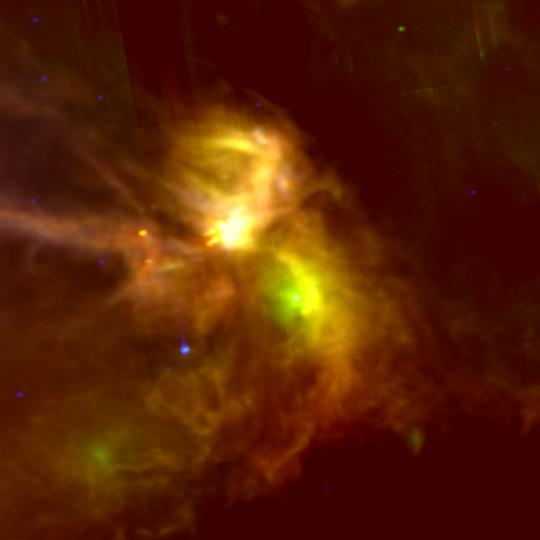
\includegraphics[width=0.4\textwidth]{../img/rho.jpg}
    \caption[An IRAS image showing the Rho Opiuchi cloud complex, the closest cloud complex to the Solar System \parencite{rho}. Rho Opiuchi is an example of a molecular cloud that is actively forming stars.]{An IRAS image showing the Rho Opiuchi cloud complex, the closest cloud complex to the Solar System \parencite{rho}. Rho Opiuchi is an example of a molecular cloud that is actively forming stars.}
    \label{fig:rho}
  \end{center}
\end{wrapfigure}

An example of a molecular cloud is shown in Figure \ref{fig:rho}. The subject of Figure \ref{fig:rho} is the Rho Ophiuchi cloud complex as imaged by the Infra-red Astronomical Satellite (IRAS). Rho Opiuchi is the nearest active star forming molecular cloud complex to the Solar System\footnote{\textcite{rho-dist} estimates the range of distances as being between 125pc-165pc - a range of almost 40\%.}. Crucially, Rho Ophiuchi is an example of a `stellar nursery`: a molecular cloud that is actively forming stars. As a result of this, Rho Ophiuchi provides an  oppurtunity to study these sites of early star formation at high resolution. This is in spite of the large uncertainty in estimates of the distance to Rho Ophiuchi \parencite{rho-dist}. Figure \ref{fig:rho} does illustrate, however, that the early stages of star formation aren't directly observable owing to their occlusion by dust in the molecular cloud. This means that the star-forming process prior to the pre-Main Sequence phase - where the star blows away its surroundings material - has yet to be directly observed, merely theorised \parencite{hayashi}. Consequently, the initial conditions for star formation to occur have yet to be constrained. Furthermore the only measure of mass distribution in the stellar environment is the Initial Mass Function \parencite{imf}, which describes the mass at which a star enters the Main-Sequence - a measure of the mass distribution prior to the Main-Sequence (the Core Mass Function) when the stellar object remains unobserved is poorly constrained in its relation to the IMF. Therefore, an alternative method of observing pre-Main Sequence objects, along with investigating the conditions within a molecular cloud at these points, is required to begin constraining both the initial conditions and the CMF. Given that dust occludes these sites, could the dust itself prove a useful tracer of the activity that it enshroudes?

\subsection{Molecular cloud composition}
Much like the ISM, molecular clouds are composed of gas and cosmic dust. Gas in the ISM is thought to be in a number of `phases`, with each phase being a different chemical composition as well as a different density and temperature. The different gaseous phases of the ISM, along with estimates of their temperature $T$ and number density $n$ are shown in Table \ref{table:ism}.

\begin{table}[h]
  \centering
   \begin{tabular}{||c c c||}
   \hline
   Component & $T\/(K)$ & $n\/(cm^{-3})$ \\ [0.5ex]
   \hline\hline
   Molecular    & $10-20$      & $10^{2}-10^{6}$ \\
   \hline
   Cold atomic  & $50-100$     & $20-50$ \\
   \hline
   Warm atomic  & $6000-10000$ & $0.2-0.5$ \\
   \hline
   Warm ionized & $\sim8000$    & $0.2-0.5$ \\
   \hline
   Hot ionised  & $\sim10^{6}$  & $\sim0.0065$ \\ [1ex]
   \hline
   \end{tabular}
   \caption{A table showing the different phases of the ISM, along with estimates of that phase`s temperature, $T$ and number density, $n$ \parencite{ism}.}
   \label{table:ism}
\end{table}

Much like gas in the interstellar medium, interstellar dust`s chemical composition varies, with theories predicting both silicate and carbonaceous species co-existing; this project assumed all dust to be of one species, and to be silicate based. As a molecular cloud is a condensation of the ISM, the composition of both remain similar, however a molecular cloud differs from the ISM in a number of key ways. Greater densities are found within a molecular cloud than that of the ISM. The gas density in the core of a molecular cloud is thought to be around $~$$1\times10^{4}\/cm^{-3}$ according to \textcite{density}, whilst the gas density in the surrounding ISM is thought to be around $10^{2}\/cm^{-3}$ as Table \ref{table:ism} shows. Assuming the dust mass to be 1\% that of the gas mass then this produces dust densities of $~$ $10^{2}\/cm^{-3}$ in dense regions of the cloud and $~$ $1\/cm^{-3}$ in the surrounding ISM.

The dust densities may be greater in a molecular cloud than the ISM, but the temperature is observed to obey a different paradigm. \textcite{dustopacity} estimates that a molecular cloud has a temperature $<$ $20\/K$, significantly cooler than the surrounding ISM as shown by Table \ref{table:ism}. The warmer ISM results in a temperature gradient; the ISM heats the cloud from the outside in, resulting in a temperature that increases with distance from the centre of the cloud.

Figure \ref{fig:rho} illustrates the intense infra-red emission within molecular clouds owing to the active star forming occurring within them. It also illustrates the turbulence and chaos within the cloud, with both filamentary structure and (potentially) magnetic fields running throughout the cloud itself. These filaments are regions of higher density, but as \textcite{evo-mol} highlights, the `edges` and transitions in molecular clouds are not strict boundaries as they may appear, but are rather molecular gas transitioning into the surrounding atomic gas. This poses an interesting question: if filaments are dense condensations of gas and dust, then do they act as preferential star formation sites? To answer this question, it is useful to review the conditions within the cloud itself that could instigate the star forming process.

\subsection{Star forming conditions} \label{sec:conditions}
\textcite{jeans} first demonstrated that a gas of given density and mass will begin to collapse if the gas pressure is overwhelmed by the gravitational force of the gas. This is applicable to star formation, given that 99\% of a molecular cloud, by mass, is gas. As a result, star forming regions within molecular clouds originate from locations of gravitational instability that lead to subsequent collapse. A stable cloud (or portion of a cloud) is in hydrostatic equilibrium, such that the force due to gravity is balanced by the force due to gaseous pressure from the gas within the cloud. This equilibrium state can also be regarded as a virialised state such that $2T+\Omega=0$, where $T$ is the total thermal energy of the system and $\Omega$ is the total gravitational potential energy of the system. The cloud begins to collapse when the gravitational force is greater than the force due to the hydrostatic pressure. This collapse continues unimpinged until such a time that another opposing force can halt the collapse. The initial collapse is triggered when a region within the molecular cloud has a mass that exceedes the Jeans` mass given by Equation \ref{eq:jeans}. This is known as the Jeans Criterion.

\begin{equation}
  M_{J} = \Bigg( \frac{5kT}{GM} \Bigg )^\frac{3}{2} \Bigg( \frac{3}{4\pi\rho} \Bigg )^\frac{1}{2}
  \label{eq:jeans}
\end{equation}

Within Equation \ref{eq:jeans}, $k$ is the Stefan-Boltzmann constant, $T$ is the temperature of the region, $G$ is the Universal Gravitational Constant, $M$ is the mass of gas (in this case $H_{2}$) in the region and $\rho$ is the density of the region prior to collapse. The radius of the region required to collapse is given in Equation \ref{eq:jeans_radius}.

\begin{equation}
  R_{J} = \Bigg ( \frac{15 k T}{4\pi G \mu m_{p} \rho} \Bigg ) ^{1/2}
  \label{eq:jeans_radius}
\end{equation}

$k$ is the Boltzmann constant, whilst $G$ is the Universal Gravitational Constant. $\mu$ is the mean molecular weight and $m_{p}$ is the mass of the proton. The collapse of an $M_{J}$ mass region occurs according to the free-fall time, $t_{ff}$ described in Equation \ref{eq:tff} \parencite{jeans}.

\begin{equation}
  t_{ff} = \sqrt{\frac{3\pi}{32G\rho}}
  \label{eq:tff}
\end{equation}

Variables within Equation \ref{eq:tff} are as they were defined in Equation \ref{eq:jeans}. As Equation \ref{eq:jeans} illustrates, the larger the temperature $T$ and the lower the gas density $\rho$, then the greater the Jeans` mass becomes, making it harder for the region to begin collapse. The temperature within the cloud itself exists as both a gas temperature and a dust temperature. \textcite{decouple} estimates that the gas within the cloud does not heat the dust within the cloud until the number density $n$ exceedes $~2\times10^{4}\/cm^{-3}$. This is defined as `thermal coupling`. The dust itself reaches thermal equilibrium when the dust heating rate per unit volume $\Gamma_{ext}$ equals the radiative cooling rate $\Lambda_{dust}$ \parencite{treecol}:

\begin{equation}
  \Gamma_{ext} - \Lambda_{dust} = 0
  \label{eq:heat}
\end{equation}

The heating mechanism of the dust is primarily through absorption of radiation, either from the Interstellar Radiation Field (a field of electomagentic radiation in the interstellar medium) or from sources of radiation within the cloud (a protostar, for example). A mathematical treatment as defined in \textcite{treecol} can be found in the Appendix. This study used an ISRF in the Arepo data but not in the isothermal sphere case discussed later (it was assumed that the dust grains in both the cloud and ISM were in thermal equilibrium such that Equation \ref{eq:heat} was satisfied).

According to \textcite{bound}, the majority of a molecular cloud remains gravitationally unbound, further reinforcing the idea stated in \textcite{evo-mol} that molecular clouds are diffuse, transiest structures. The onset of gravitational binding is also not a singular process. A region of a molecular cloud may begin to collapse under the Jeans criterion in Equation \ref{eq:jeans}, however this clump may then sub-fragment into smaller clumps that also begin collapsing in a similar manner. Whether a given clump is gravitationally bound or not is a measure of whether that clump is a prestellar core or not, according to \textcite{prestellar}. \textcite{prestellar} also states that the majority of prestellar cores remain starless - even so, even fewer cores will evolve to become protostellar cores and begin the route to the Main-Sequence. Those prestellar cores that do not evolve to form protostellar cores are thought to disperse before they're ever able to form stars.

The conditions that harbour these star forming regions are difficult to observe directly because of their obscuration by the enveloping dust. Gas is responsible for the collapse of the medium (via the Jeans Criterion in Equation \ref{eq:jeans}) and formation of the star itself, however dust absorbs the emission from these collapsing regions, essentially masking them. The dust itself will, however, re-radiate the absorbed radiation incident upon it at a sub-mm/IR wavelength.

\section{Dust emission}
Dust is a relatively small fraction of the total ISM mass, estimated as being only 1\% according to \textcite{noise}. Whilst the dust mass accounts for such a small mass component, it still presents an important role in forming stars. The sources of flux embedded deep within the cloud radiate across a wide range of wavelengths, however the dust surrounding the source has the effect of absorbing and then re-radiating photons at a different (longer) wavelength. As such, these sources of flux (be they prestellar cores or protostars) are occluded by the dust enveloping them.

According to \textcite{dustopacity}, dust radiates as a modified black body in the far infra-red regime (i.e. from $\lambda=\SI{60}{\micro\meter}$) that can approximated using Equation \ref{eq:mbb}.

\begin{equation}
  S_{\nu} = N_{H_{2}} \Omega \kappa_{0} \Big(\frac{\nu}{\nu_{0}}\Big)^{\beta} B_{\nu}(T)
   \label{eq:mbb}
\end{equation}

In Equation \ref{eq:mbb} $S_{\nu}$ is the flux density, $N_{H_{2}}$ is the column density of molecular Hydrogen, $\Omega$ is the solid angle subtended by the beam, $\kappa_{0}$ is a reference dust opacity, $\nu$ is the frequency of the image, $\nu_{0}$ is a reference frequency at which the reference opacity $\kappa_{0}$ was evaluated at, $\beta$ is the dust spectral index (for siliciate and carbonaceous grains, \textcite{beta} approximates $\beta \sim 2$) and $B_{\nu}(T)$ is the frequency dependent Planck function. An assumption made here, as stated by \textcite{kelly}, is that the dust is optically thin such that
$\tau_{\nu} = N\kappa_{\nu} \ll 1$. The term $\kappa_{0}(\frac{\nu}{\nu_{0}})^{\beta}$ is the Hildebrand dust opacity law $\kappa_{\nu}$ given in \textcite{dustopacity}. In terms of intensity this equation becomes:

\begin{equation}
  I_{\nu} = \frac{N_{H_{2}}}{R_{dust-gas}} \mu m_{p} \kappa_{0} \Big(\frac{\nu}{\nu_{0}}\Big)^{\beta} B_{\nu}(T)
   \label{eq:mbb-int}
\end{equation}

All variables in Equation \ref{eq:mbb-int} are as defined in Equation \ref{eq:mbb}, with the addition of $R_{dust-gas}$. $R_{dust-gas}$ is the dust-to-gas ratio, here approximated as being $100$. We observe that $\frac{N_{H_{2}}}{R_{dust-gas}}$ is the column density of dust along the line of sight, $N$. It is this parameter (along with $T$ along the line of sight) that are the focii of this project. Furthermore throughout this project dust emission was quantified in terms of intensity rather than flux density, as intensity is independent of distance to the source of emission.

\begin{wrapfigure}{l}{0.4\textwidth}
    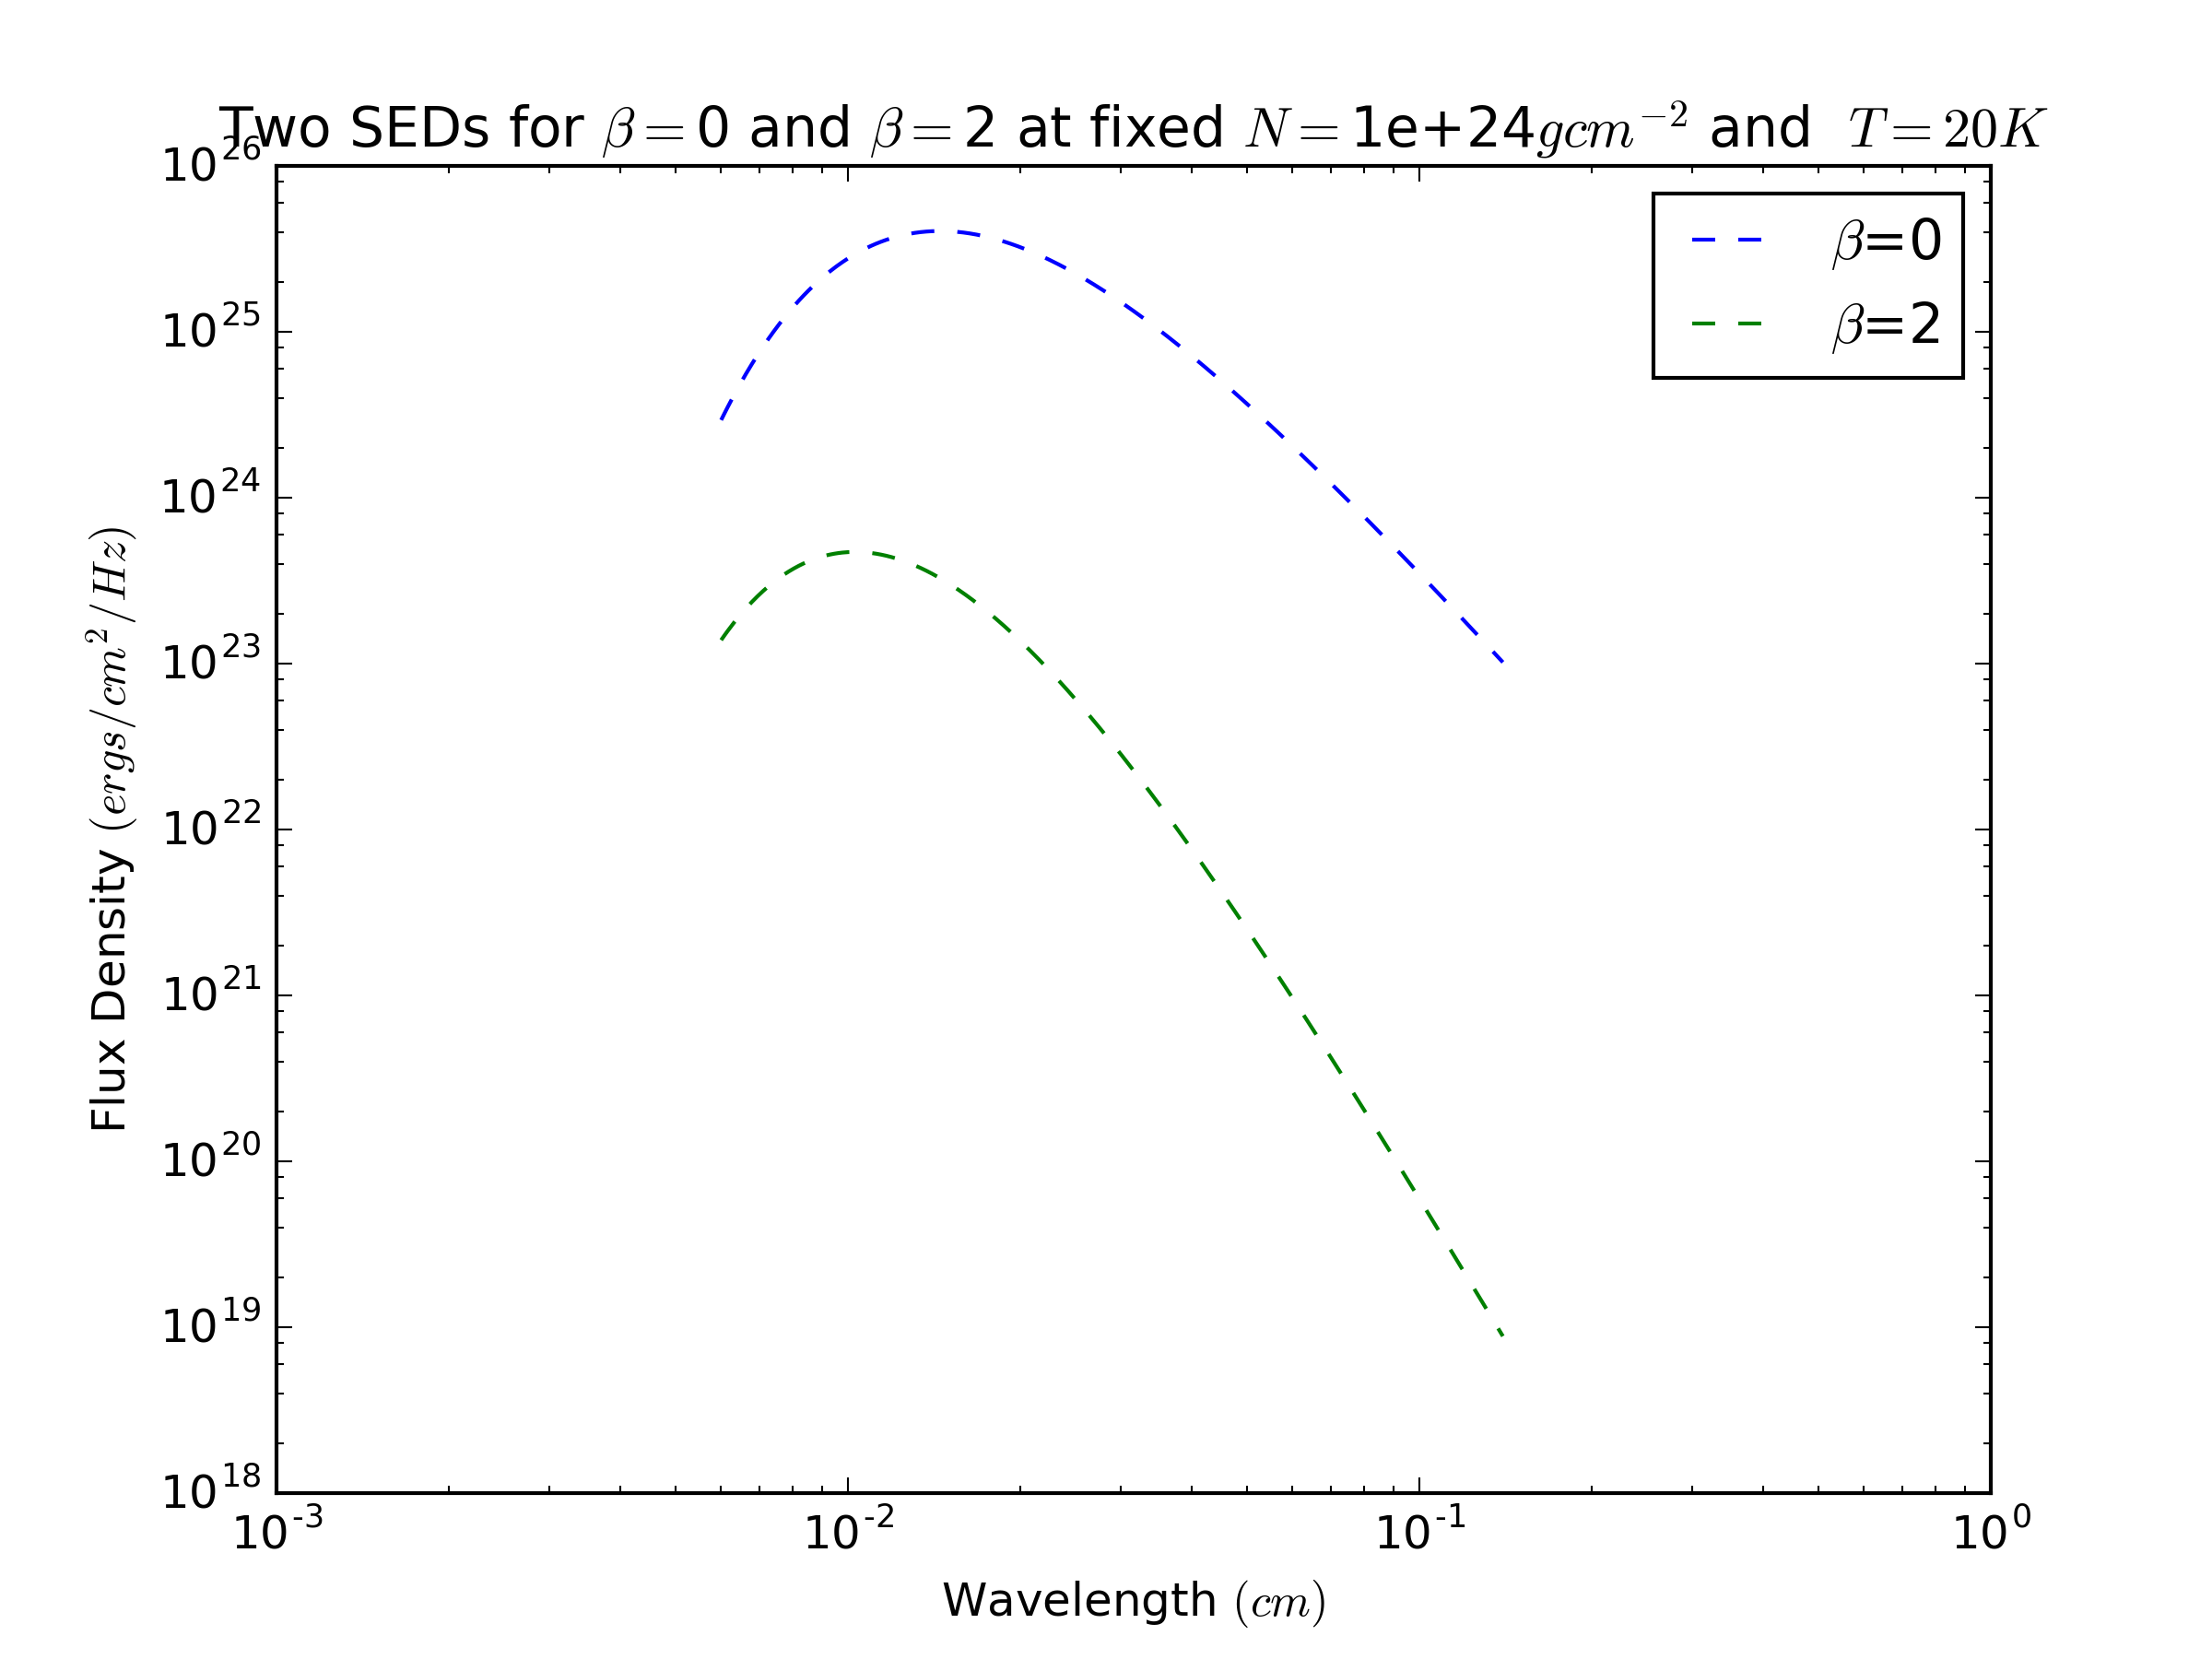
\includegraphics[width=0.4\textwidth]{../img/flux_density_combined.png}
    \caption[A plot illustrating how the dust spectral index $\beta$ varies the emergent dust SED whilst both $N$ and $T$ remain fixed. This is based off of a plot found in \textcite{noise}.]{A plot illustrating how the dust spectral index $\beta$ varies the emergent dust SED whilst both $N$ and $T$ remain fixed. This is based off of a plot found in \textcite{noise}.}
     \label{fig:beta-ex}
\end{wrapfigure}

Dust properties such as the spectral index $\beta$, temperature $T$ and column density $N$ clearly have an effect on dust emission according to Equations \ref{eq:mbb} and \ref{eq:mbb-int}. Importantly, both Equations \ref{eq:mbb} and \ref{eq:mbb-int} describe dust emission at a single temperature $T$. Two emergent SEDs described by Equation \ref{eq:mbb} at fixed single $N$ and $T$ are shown in Figure \ref{fig:beta-ex}. These properties, however, are experimentally difficult to measure and
\textcite{kelly} states that most observational attempts to determine $T$ and $\beta$ rely on a $\chi^{2}$ SED fitting routine. This routine does, however, suffer from drawbacks when fitting for a single temperature $T$. To illustrate, consider Figure \ref{fig:col}.

\begin{figure}[h]
  \begin{center}
    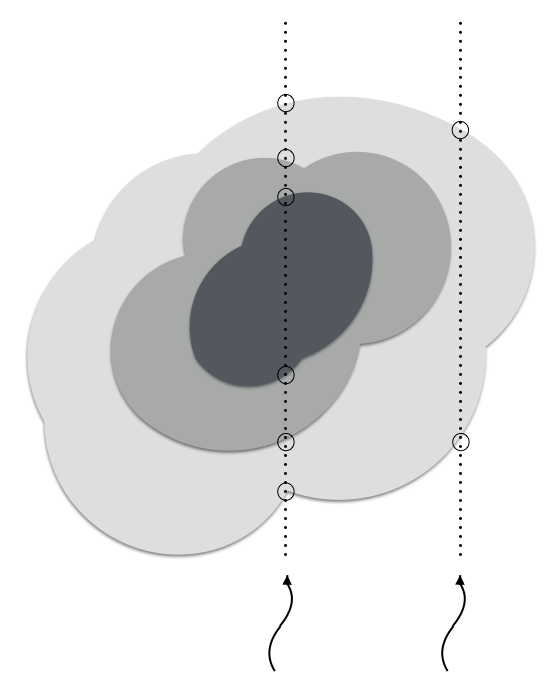
\includegraphics[width=0.3\textwidth]{../img/column.png}
    \caption[A figure illustrating a basic molecular cloud, with regions of higher density denoted by darker regions. Solid black lines indicate an incoming photon, whilst a dashed line indicates the line of sight.]{A figure illustrating a basic molecular cloud, with regions of higher density denoyed by darker red regions. Solid black lines indicate an incoming photon, whilst a dashed line indicates the line of sight.}
    \label{fig:col}
  \end{center}
\end{figure}

Figure \ref{fig:col} shows a basic molecular cloud with sub-structure (and therefore increasing density) illustrated by the consecutively darker regions. A circle indicates the point at which a photon, or indeed the line of sight, passes from a region of one density to a region of different density. By using the line of sight through the centre of the cloud, it is observed that this line of sight intersects a larger number of boundaries than the line of sight on the right that only passes through one region. This means that a larger $N$ is observed through the line of sight in the middle of the cloud than the line of sight on the right. Furthermore, the greater number of boundaries present greater opportunity for the photon to reflect/scatter. This means that the photon is not absorbed by the dust grain and therefore does not heat it. The larger number of boundaries through the central line of sight means that the material in regions of higher density are not heated as much as the material at lower density, for example the region intersected by the right hand line of sight. This has the effect of introducing more temperature variations along the line of sight when $N$ is large in comparison to low $N$. Therefore, single $T$ fits (in the case of a $\chi^{2}$ fit) in regions of low $N$ recover accurate $T$, whereas single $T$ fits in regions of high $N$ are overestimated owing to the line of sight temperature variations. This effect is observed in studies by \textcite{noise,noiseb} and \textcite{kelly} by fitting for $\beta$-$T$.

\subsection{The $\beta$-$T$ degeneracy} \label{sec:degen}
As Equation \ref{eq:mbb-int} shows, dust does not radiate as a perfect blackbody. This is accounted for by multiplying the Planck function (i.e. the function that describes a body that radiates as a perfect blackbody) by the dust opacity term $\kappa = \kappa_{0}(\frac{\nu}{\nu_{0}})^{\beta}$. Two key variables here are the dust spectral index $\beta$ and the dust temperature $T$. These two properties suffer from a degeneracy \parencite{degen} such that any $\chi^{2}$ test applied to determining the values of $\beta$ and $T$ may understimate one parameter whilst overestimating another.

As \textcite{noise} states, a fitting routine for $\beta$ and $T$ is prone to overestimates owing to the assumption that temperature is constant along the line of sight. For an isothermal source this assumption may be well placed however in the case of a complex structure such as a molecular cloud shown in Figure \ref{fig:rho} this assumption is inaccurate. Equations \ref{eq:mbb} and \ref{eq:mbb-int} describe dust emission from an isothermal source, i.e. one in which the dust is at one discrete temperature. Molecular clouds are not isothermal and have a range of temperatures along the line of sight, and as \textcite{noise} highlights, the SEDs describing the dust emission in these instances are actually combinations of the individual SEDs from each individual temperature source. Observing these sources directly accounts for this, and one such way to observe a molecular cloud in reality is via the Herschel Space Observatory.

\section{Herchel Space Observatory}
The Herschel Space Observatory was an ESA mission launched in 2009 with the primary objective of imaging cold regions of the Universe \parencite{herschel,fact}. Herschel had a number of objectives, including observing sites of early star formation to understand the initial conditions that establishes star formation itself \parencite{fact}. To achieve this, Herschel was launched with 3 different instruments onboard: Photodetector Array Camera and Spectrometer: PACS \parencite{PACS}, Spectral and Photometric Imaging Receiver: SPIRE \parencite{SPIRE} and Heterodyne Instrument for the Far Infrared: HiFi \parencite{HiFi}. One of these instruments, SPIRE, was designed to probe the sites of early star formation deep within molecular clouds. This was achieved by imaging solely in the infra-red and sub-mm regimes. Herschel itself, across all instruments and functional modes, is sensitive to a range of wavelengths quoted by \textcite{herschel} as $\sim \SI{55}{\micro\meter}$ to $\sim \SI{672}{\micro\meter}$. Both PACS and SPIRE were capable of being run in ``Parallel mode'' - effective simultaneous operation according to \textcite{herschel}. SPIRE itself had an photometry wavelength range
$\sim \SI{200}{\micro\meter}$ to $\sim \SI{670}{\micro\meter}$ whilst PACS was sensitive to a photometry wavelength range $\sim \SI{60}{\micro\meter}$ to $\sim \SI{210}{\micro\meter}$. This therefore produces effectively continuous coverage of the wavelength range $\sim \SI{60}{\micro\meter}$ to $\sim \SI{670}{\micro\meter}$.
\footnote{Further coverage is achieved down to $\SI{55}{\micro\meter}$ using HiFi however this is only achievable for spectroscopic applications.}

Tables \ref{table:SPIRE-pass} and \ref{table:PACS-pass} illustrates the passbands for each of the filters within SPIRE and PACS.

\begin{table}[h]
  \captionsetup{width=0.3\textwidth}
  \parbox{.4\linewidth}{
  \centering
  \begin{tabular}{||l l||}
  \hline
  Filter & Passband ($\mu m$) \\ [0.5ex]
  \hline\hline
  PSW    &    199.4540 --	298.5657   \\
  \hline
  PMW    &    281.6949 --	424.7548   \\
  \hline
  PLW    &    391.4346 --	690.8139   \\ [1ex]
  \hline
  \end{tabular}
  \caption{\protect The passbands (for extended source) for the SPIRE instrument \parencite{pass}.}
  \label{table:SPIRE-pass}
  }
  \parbox{.4\linewidth}{
  \centering
  \begin{tabular}{||l l||}
  \hline
  Filter & Passband ($\mu m$) \\ [0.5ex]
  \hline\hline
  Blue   &    55.6706 -- 97.7403       \\
  \hline
  Green  &    79.1026 --	135.1498     \\
  \hline
  Red    &    117.7762 --	243.6431     \\ [1ex]
  \hline
  \end{tabular}
  \caption{\protect The passbands for the PACS instrument \parencite{pass}.}
  \label{table:PACS-pass}
  }
\end{table}

In order to achieve the effective wavelength range described in Tables \ref{table:SPIRE-pass} and \ref{table:PACS-pass}, both SPIRE and PACS detectors required extensive cooling to a temperature of $0.3 K$ via $^{3}{He}$ coolers \parencite{herschel}. Again according to \textcite{herschel} the image focal plane required cooling to $1.7 K$, again achieved using 2160 litres of Helium cryogen. To minimise any thermal radiation from the observatory itself, the spacecraft was radiatively cooled to a temperature of $85 K$ \parencite{herschel}. These temperatures allowed effective detection (via a bolometric detector in the case of SPIRE and a photometer in the case of PACS) of infra-red and sub-mm photons. As this project did not use real Herschel data, a method of not only simulating dust emission intensity but also generating realistic images was required. This was achieved by using RADMC-3D.

\section{RADMC-3D} \label{radmc}
RADMC-3D is a 3-dimensional Monte-Carlo radiative transfer and ray tracing code developed by Cornelis Dullemond for radiative transfer and emission astrophysics in dusty environments \parencite{RADMC-3D}.

RADMC-3D is able to compute dust emission intensity as well as Spectral Energy Distributions (SED) and spectra for a number of different continua. This project focussed only on dust continuum. Gas emits radiation in lines rather than continua, and therefore an SED cannot be used to recover physical gas properties directly. Furthermore, the dust and gas temperatures remain uncoupled at the densities considered in this project meaning that their temperatures differ, resulting in their emission being in different wavelength ranges. The dust emission intensity can be computed using 2 different methods: the thermal Monte-Carlo simulation, or an image ray trace. All computations, regardless of whether a Monte Carlo simulation or raytrace, require input files for RADMC-3D to read and use in its simulations.

\subsection{Input files} \label{inp}
As stated in Section \ref{radmc}, RADMC-3D requires a number of user defined input files in order to operate. These input files act as parameter spaces, defining boundary conditions along with step sizes for each given input file. Figure \ref{fig:radmc3d-workflow} shows the workflow used in this project, including all files that are required in order to operate RADMC-3D.

\begin{figure}[h]
  \centering
  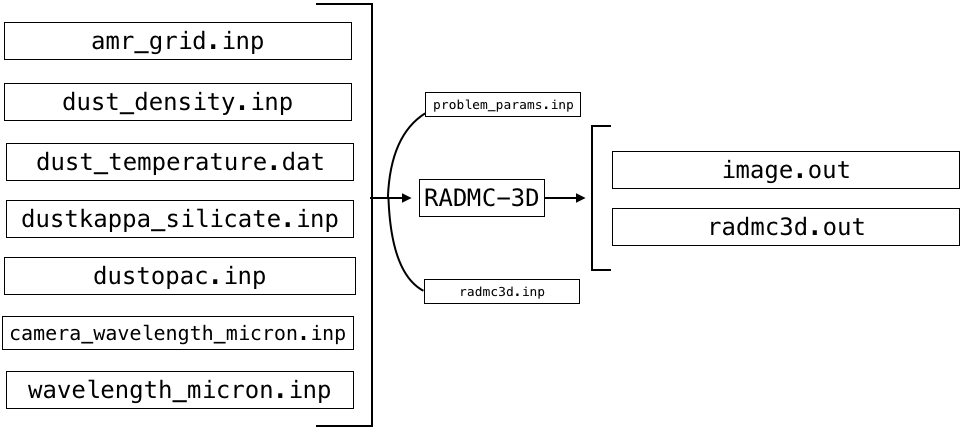
\includegraphics[scale=0.4]{../img/radmc3d-workflow}
  \caption[A schematic representation of the RADMC-3D workflow.]{A schematic representation of the RADMC-3D workflow.}
  \label{fig:radmc3d-workflow}
\end{figure}

As Figure \ref{fig:radmc3d-workflow} illustrates, all input files to RADMC-3D have extension \texttt{.inp} whilst all output files have extension \texttt{.out}. Any file that RADMC-3D is able to modify, such as those directly calculated by RADMC-3D, have extension \texttt{.dat}. \textit{Most} input files' initial lines - the header information - contain quantitative information regarding the number of pixels/cells in the file, the pixel/cell width along with other identifiers that inform RADMC-3D whether to look for binary files, the number of dust species being considered as well as the number of datapoints in the file.

\begin{wrapfigure}{r}{0.4\textwidth}
  \centering
  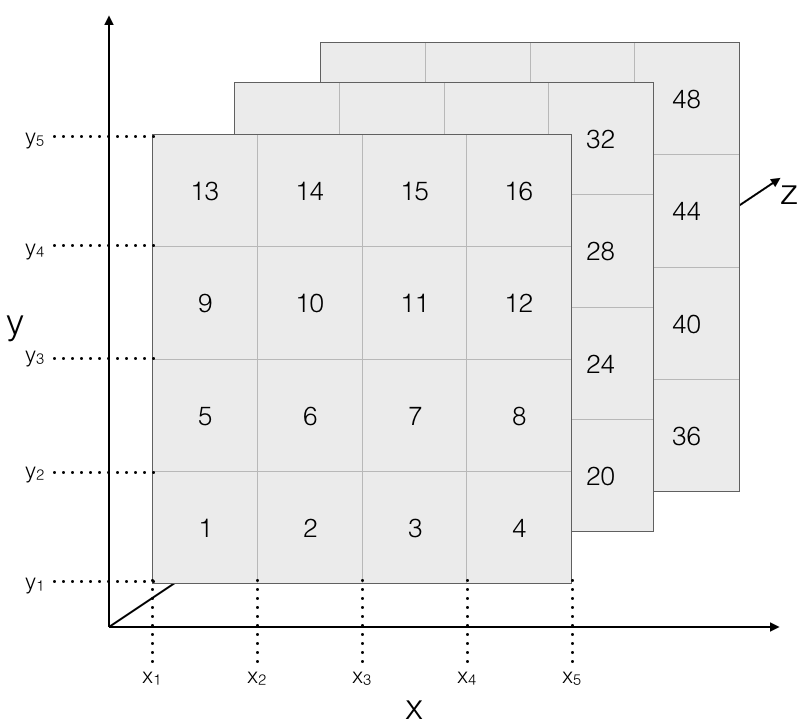
\includegraphics[scale=0.3]{../img/amr_grid_structure}
  \caption[A pictorial representation of the structure of \texttt{amr\_grid.inp} for a 4x4x3 grid. The index of a cell, denoted by the number contained within it, is the position of that cell in \texttt{amr\_grid.inp}. This image is based off of an image in \textcite{manual}.]{A pictorial representation of the structure of \texttt{amr\_grid.inp} for a 4x4x3 grid. The index of a cell, denoted by the number contained within it, is the position of that cell in \texttt{amr\_grid.inp}. This image is based off of an image in \textcite{manual}.}
  \label{fig:amr_grid_structure}
\end{wrapfigure}

\texttt{amr\_grid.inp} is the file used in order to create a spatial domain within the model. It does this by defining the start and end points of pixels in 3 dimensions: x, y and z. These definitions produce pixels, each of fixed width defined by the distance between pixel start and end points. RADMC-3D also has the ability to perform Adaptive Mesh Refinement, such that regions of interest can be split into more pixels (and have a smaller pixel width and therefore simulated higher resolutions) than, for example, regions of the ISM that do not require a higher resolution. Any further files that setup physical quantities draw directly from the structure of \texttt{amr\_grid.inp}. They essentially \textquotesingle insert\textquotesingle a value of a physical quantity into each cell, therefore producing another parameter space. This structure is illustrated in Figure \ref{fig:amr_grid_structure}.

The index of each cell in Figure \ref{fig:amr_grid_structure} is that cell's position in \texttt{amr\_grid.inp}. For example,

\texttt{dust\_density.inp} is the file that gives RADMC-3D its density information. It has the same structure as \texttt{amr\_grid.inp}, however in place of the start and end pixel points that are found in \texttt{amr\_grid.inp}, \texttt{dust\_density.inp} defines the dust density (in $cgs$ units) at each pixel. This therefore creates a density parameter space with which to work from. Similarly, \texttt{dust\_temperature.dat} draws upon the same idea, however instead of defining dust densities, \texttt{dust\_temperature.dat} defines the dust temperature (in $K$) at each pixel point. These 3 files therefore create 3 parameter spaces: spatial, density and temperature.

Another crucial file is the \texttt{wavelength\_micron.inp} file. This input file defines the wavelengths over which RADMC-3D should determine dust emission intensity. By default, \texttt{wavelength\_micron.inp} runs from $\SI{0.1}{\micro\meter}$ to $\SI{1000}{\micro\meter}$ with $150$ points. Dust emission intensity can then be determined at any wavelength between these two bounds. In reality however, computing dust emission intensity over such a wide wavelength range is not always necessary (or practical). RADMC-3D thus allows the user to define a \texttt{camera\_wavelength\_micron.inp} file. This file is designed to constrict the range of wavelengths over which RADMC-3D computes, thus emulating the wavelengths available to a given telescope or filter. In this project \texttt{camera\_wavelength\_micron.inp} was used in order to allow RADMC-3D to compute dust emission intensity in wavelength bands corresponding to those found on both SPIRE \parencite{SPIRE} and PACS \parencite{PACS}.

\subsection{Ray tracing dust emission} \label{sec:rt_des}
Whilst RADMC-3D is capable of performing a full thermal Monte-Carlo simulation to determine dust temperature, it is also capable of an image ray trace that reads in both user-defined dust temperatures and dust densities, thus bypassing the computation of the dust temperatures. This project made use of the image raytrace rather than the Monte-Carlo simulation. In the case of the isothermal sphere, temperatures are user generated from idealised estimates of temperature, whilst temperatures are generated from a thermal Monte Carlo simulation in the case of the Arepo data. According to \textcite{manual}, the ray-trace follows, by default, a first-order integration where the source function, $S = j_{\nu}/\alpha$ and opacity (and therefore extinction $\alpha$) are constant across the ray. This is described by Equation \ref{eq:raytrace}.

\begin{equation}
  I_{result} = I_{start}e^{-\tau}+(1+e^{-\tau})S
  \label{eq:raytrace}
\end{equation}

$I_{result}$ is the dust emission intensity of the cell, $I_{start}$ is the dust emission intensity of the cell prior to the ray entering it and $\tau$ is the optical depth along the path of the ray through the cell. The optical depth $\tau$ is defined as $\tau = \alpha s$ where $\alpha$ is as defined earlier and $s$ is the distance the ray travels through the cell. The option to perform second-order integration is also made possible by varying the source function $S$ and extinction across the ray. Specifically $S$ and $\alpha$ are fixed at the ingress and egress points of the ray. These points act as boundary conditions such that the variation in $S$ amd $\alpha$ can then be linearly interpolated across the path of the ray through the cell.

The result, however, is the same in both Thermal Monte-Carlo simulation and ray-trace: an \texttt{image.out} file that contains the dust emission intensity at each cell in the image plane. RADMC-3D is also capable of accounting for scattering of photons off of dust grains however this project focussed solely upon absorption and re-emission only.

%-----------------------------------------------------------------
% Methodology
%-----------------------------------------------------------------

\chapter{Methodology}
\section{Modelling routine}
This project uses a $\chi^{2}$ routine to determine $N$ and $T$ from synthetic observations. This process is the same as that used to derive $N$, $T$ or even $\beta$ in `real` observations \parencite{noise,noiseb}. As mentioned in Section \ref{sec:degen}, a single $T$ $\chi^{2}$ routine overestimates $N$ and $T$ owing to the line of sight temperature variations. As a result, an assessment of how well the $\chi^{2}$ results compare to the input quantities in the absence of line of sight temperature variations can be achieved with a simple, isothermal cloud of uniform density and temperature placed within a medium of greater temperature and lower density. This effectively simulates a cold and dense molecular cloud surrounded by a warmer, diffuse ISM.

\begin{comment}
\subsection{Example scripts}
  RADMC-3D includes a number of basic example scripts to familiarise the user with the software's operation and capabilities. As a result, they provide an excellent introductory exercise to using RADMC-3D. Examples of 1D and 2D thermal Monte-Carlo simulations were run in this regard, generating Figures \ref{fig:1d} and \ref{fig:2d}.

  \begin{figure}[!htb]
  \minipage{0.48\textwidth}
    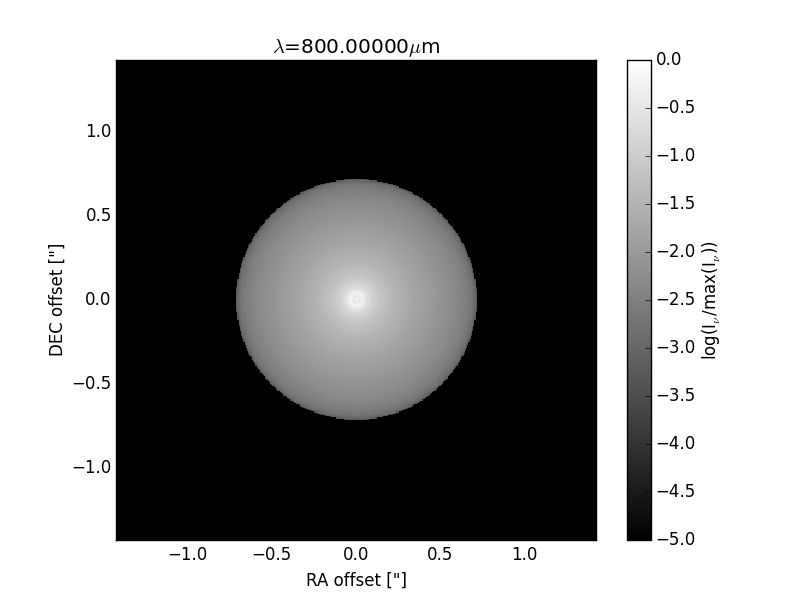
\includegraphics[width=\linewidth]{../img/1d}
    \caption{The RADMC-3D output for dust emission intensity computed using thermal Monte-Carlo simulation in 1D.}\label{fig:1d}
  \endminipage\hfill
  \minipage{0.48\textwidth}
    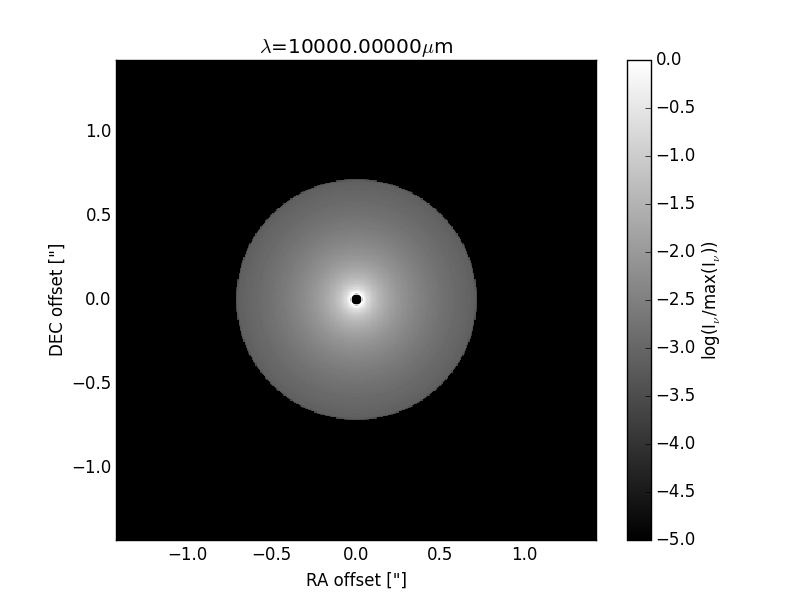
\includegraphics[width=\linewidth]{../img/2d}
    \caption{The RADMC-3D output for dust emission intensity computed using thermal Monte-Carlo simulation in 2D.}\label{fig:2d}
  \endminipage
  \end{figure}

  In order to begin operation, RADMC-3D's example scripts were analysed and run. The examples were used to understand how RADMC-3D generated the input files required (and as discussed in Section \ref{inp}) as well as how the code used them and for what purpose. These examples were basic, consisting of both 1D and 2D sphere projections with user defined stars at their centres.

  These examples ran thermal Monte-Carlo simulations. The first stage in this computation after writing the input files from the user inputs was to build dust temperatures. This was achieved using the process described in Section \ref{mctherm}. Once dust temperatures had been computed, RADMC-3D then performed a ray-trace in order to build the dust emission intensity. This was again achieved using the method described in Section \ref{rt_des}.
\end{comment}

\subsection{Modelling a cloud}
Modelling an isothermal cloud can be split into 3 distinct stages:

\begin{enumerate}
  \item Generate input files to create parameter spaces for RADMC-3D
  \item Perform ray-trace on these files, at each of the SPIRE and PACS bands, to build dust emission intensities
  \item Account for the filter transmission to `degrade` the intensities, and reduce these datapoints to one discrete, effective wavelength as SPIRE/PACS would observe
\end{enumerate}

\begin{comment}
  To begin building 3D models outside of the example scripts, specific input files needed to be created. As stated, a custom Python script \texttt{datafilegen.py} was written to handle this file creation. Traditionally, \texttt{radmc3dPy} would handle file creation at the model setup phase, however given that RADMC-3D is designed to be run from the command line it was determined that reducing the number of dependencies would allow greater compatibility with different machines. This is critical if the code was to be run on a machine that may not have \texttt{radmc3dPy} installed, such as a supercomputer for larger computations. This also resulted in some of \texttt{radmc3dPy\textquotesingle s} model setup commands being made redundant. For example, \texttt{radmc3dPy.setup.problemSetupDust} sets up the model using input parameters that are parsed to a model file. This phase was handled solely by \texttt{datafilegen.py}, so this command was redundant. Instead, required parameters such as the number of pixels in each dimension was given to RADMC-3D when calling it from the command line using \texttt{os.system(radmc3d image loadlambda)}. Again, the image ray-trace could be initiated through Python via the \texttt{os.system(radmc3d image)} command. The \texttt{loadlambda} keyword informs RADMC-3D that it should use the \texttt{camera\_wavelength\_micron.inp} module.
\end{comment}

\subsection{Building dust intensities}
By suppling RADMC-3D with initial input files to build parameter spaces, the code can then perform its raytrace using the method discussed in Section \ref{sec:rt_des}. The output, \texttt{image.out}, is a 2D image with image dimensions in the x-y plane corresponding to the initial x and y image dimensions supplied to RADMC-3D. This file contains the dust emission intensity values at each pixel within that plane. This intensity is, however, an idealised intensity that does not account for any ineffeciences. It was necessary therefore in order to simulate data as imaged by Herschel to account for the frequency dependent transmission of Herschel's filters.

\subsection{Simulating Herschel}
No telescope or observatory can produce perfect images or data; components within the telescope, the observatory or the surroundings all degrade the data quality. In real world applications maximising the SNR is crucial to data quality, but the principles of this will not be touched on here. Furthermore SNR (and therefore integration time) is not accounted for in the simulations or data analysis - images are plotted as if the source is integrated for sufficient time such that the fictional `detector` responds and detects all photons from the source incident upon it as they were emitted from the dust. It was also assumed that the source is imaged in the absence of any occluding material along the line of sight between the observer and the source, and thus exctinction was neglected.

Naturally this is an idealised assumption; not all photons that fall on a detector are detected. Detectors have a given responsivity that is a measure of how many of the incident photons contribute to the signal. Furthermore, filters are essential to telescope operation as they discriminate wanted and unwanted frequencies to ensure only frequencies within the passband of interest are transmitted to the detector. This introduces a large inefficiency in that not all incident photons are transmitted owing to reflection off of the filter itself, as well as absorption within the filter. This is frequency dependent and thus produces a ``transmission curve''.

\subsection{Accounting for filter transmission}
Whilst the detector`s filter permits only photons of the required frequencies to the detector by reflecting the unwanted photons, it also has the effect of reducing the intensity of the photons that are permitted through it. This can be described via a transmission curve, which varies depending on the filter under consideration. The transmission curve itself describes the transmission coefficient at each wavelength/frequency in the band, which is simply $\frac{I_{f}}{I_{i}}$ where $I_{f}$ is the intensity of the incoming wave and $I_{i}$ is the intensity of the wave prior to entering the filter. Figure \ref{fig:transmission} shows the transmission curves as a function of frequency for each of the 6 bands considered in this project.

\begin{figure}
\centering

\begin{subfigure}[b]{.45\linewidth}
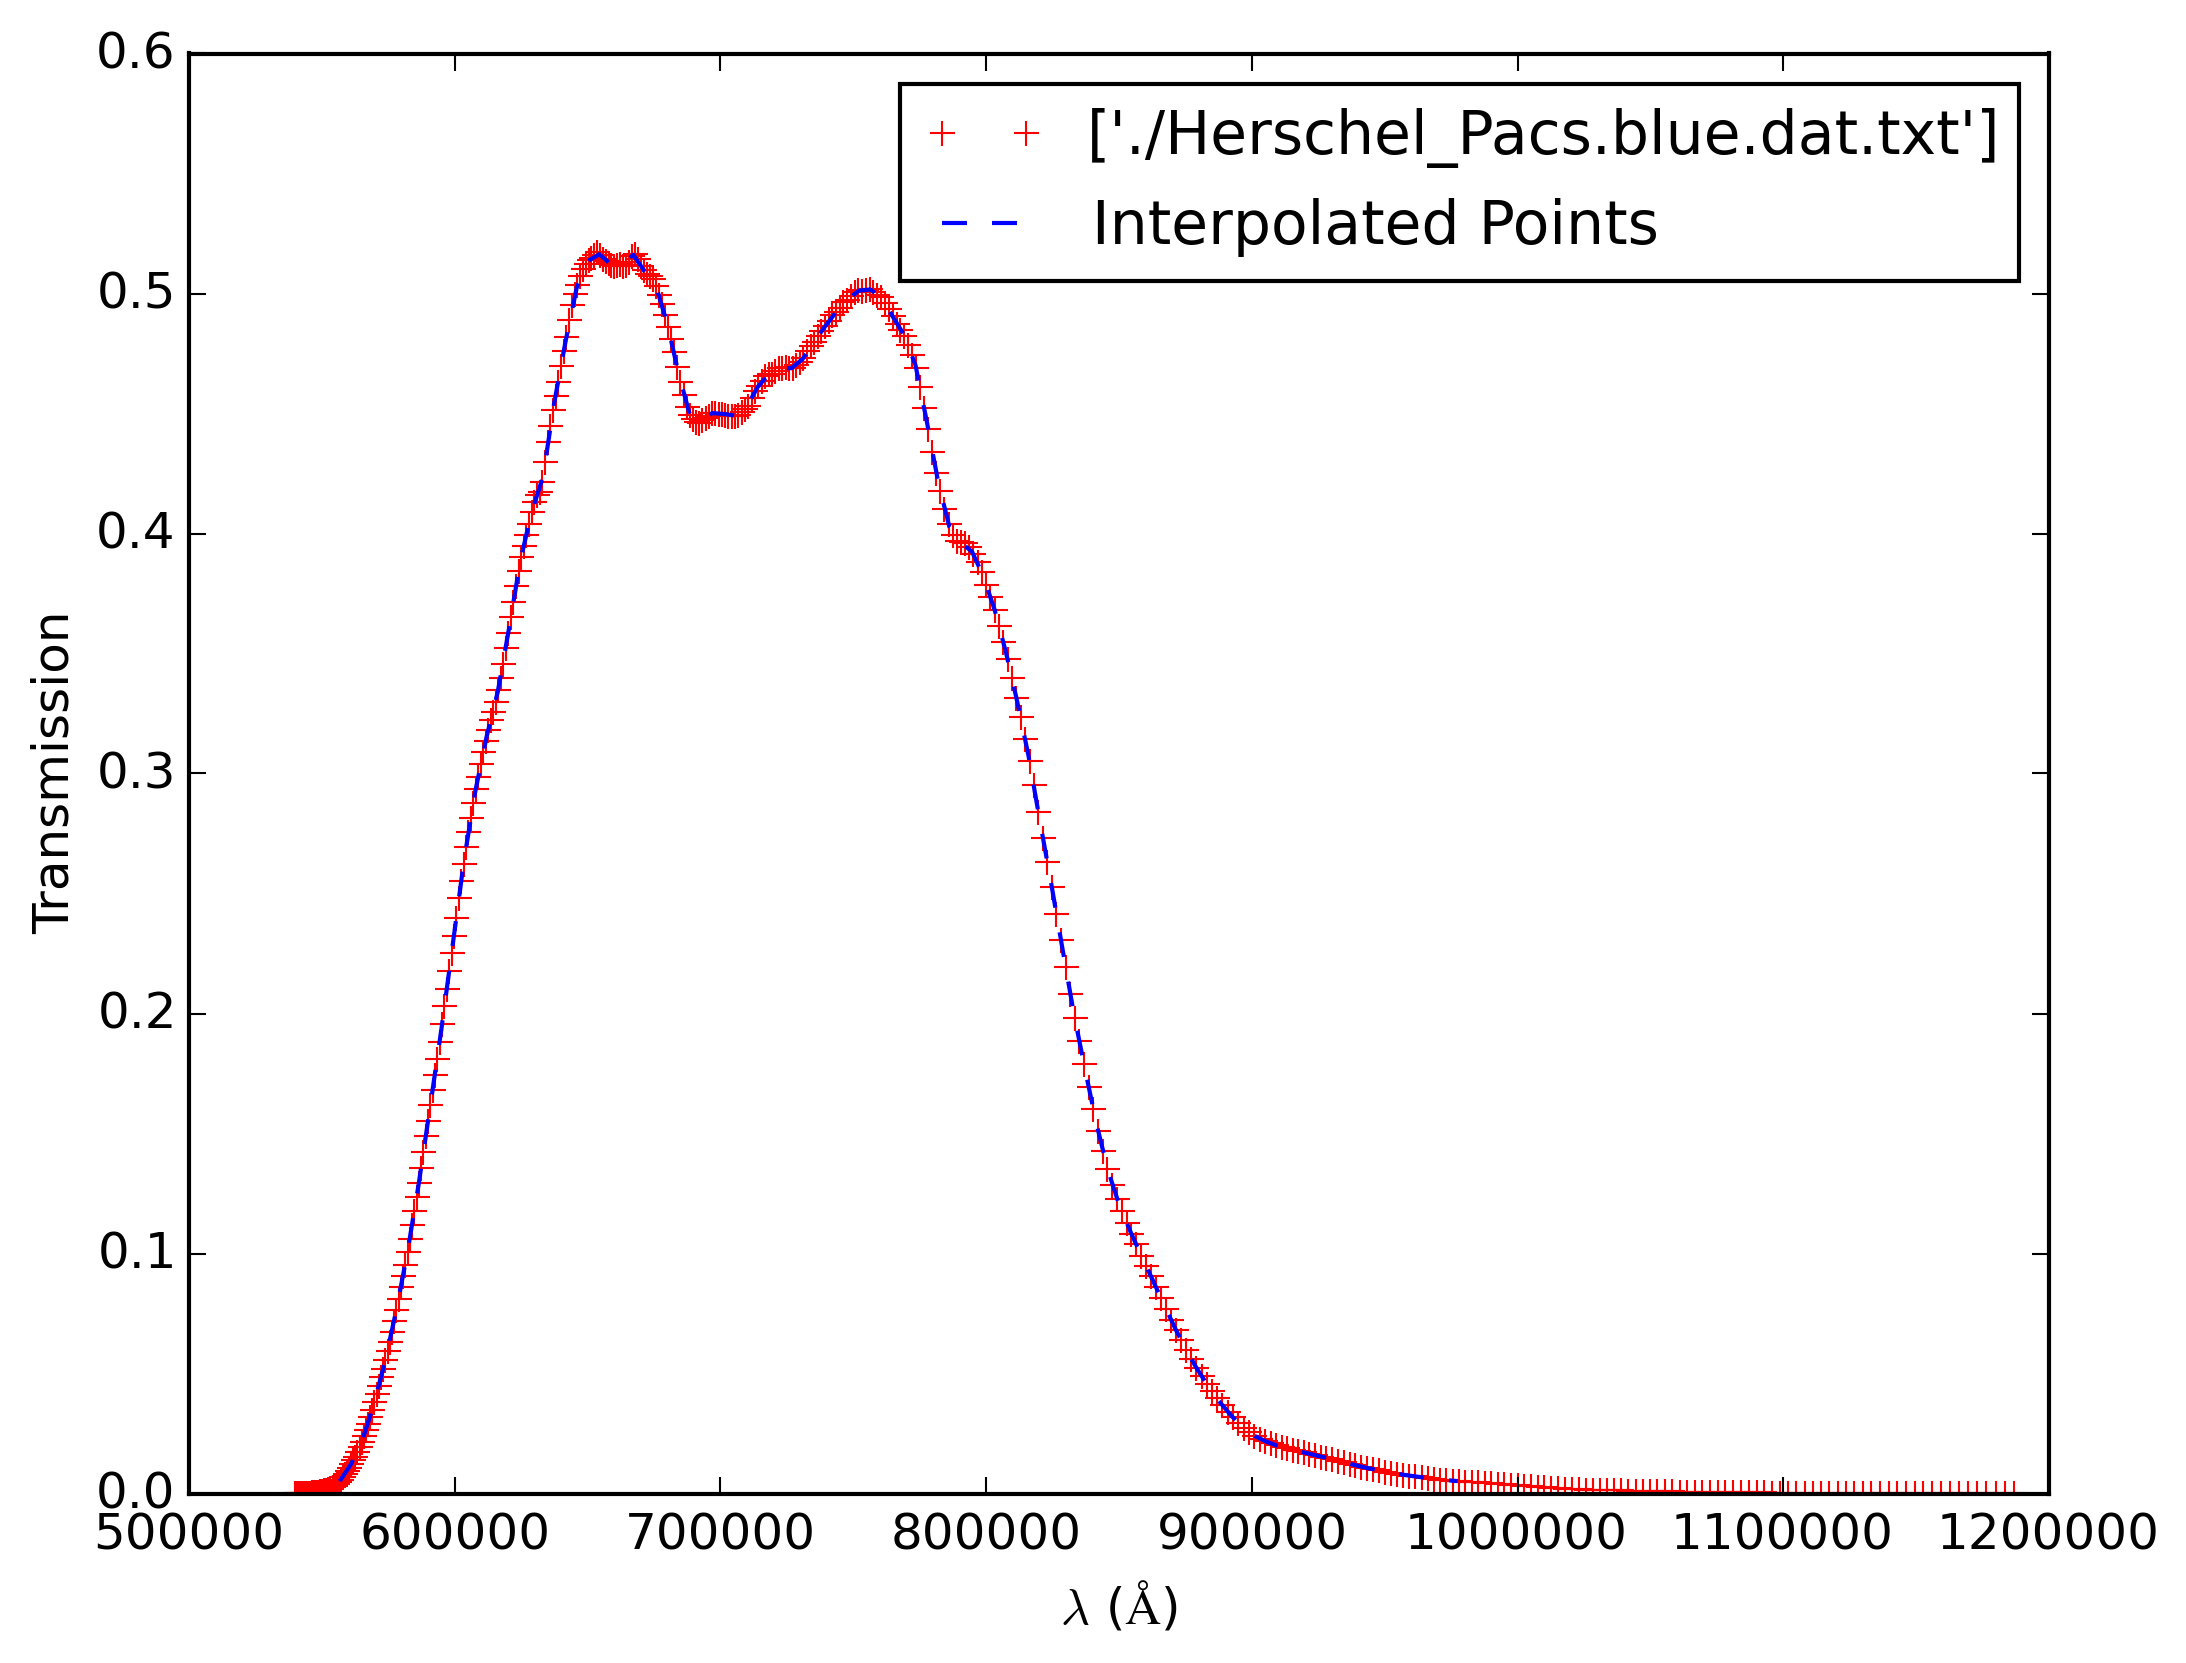
\includegraphics[width=\linewidth]{../img/interpolated_blue.png}
\caption{The transmission curve for the PACS Blue band.}\label{fig:blue}
\end{subfigure}
\begin{subfigure}[b]{.45\linewidth}
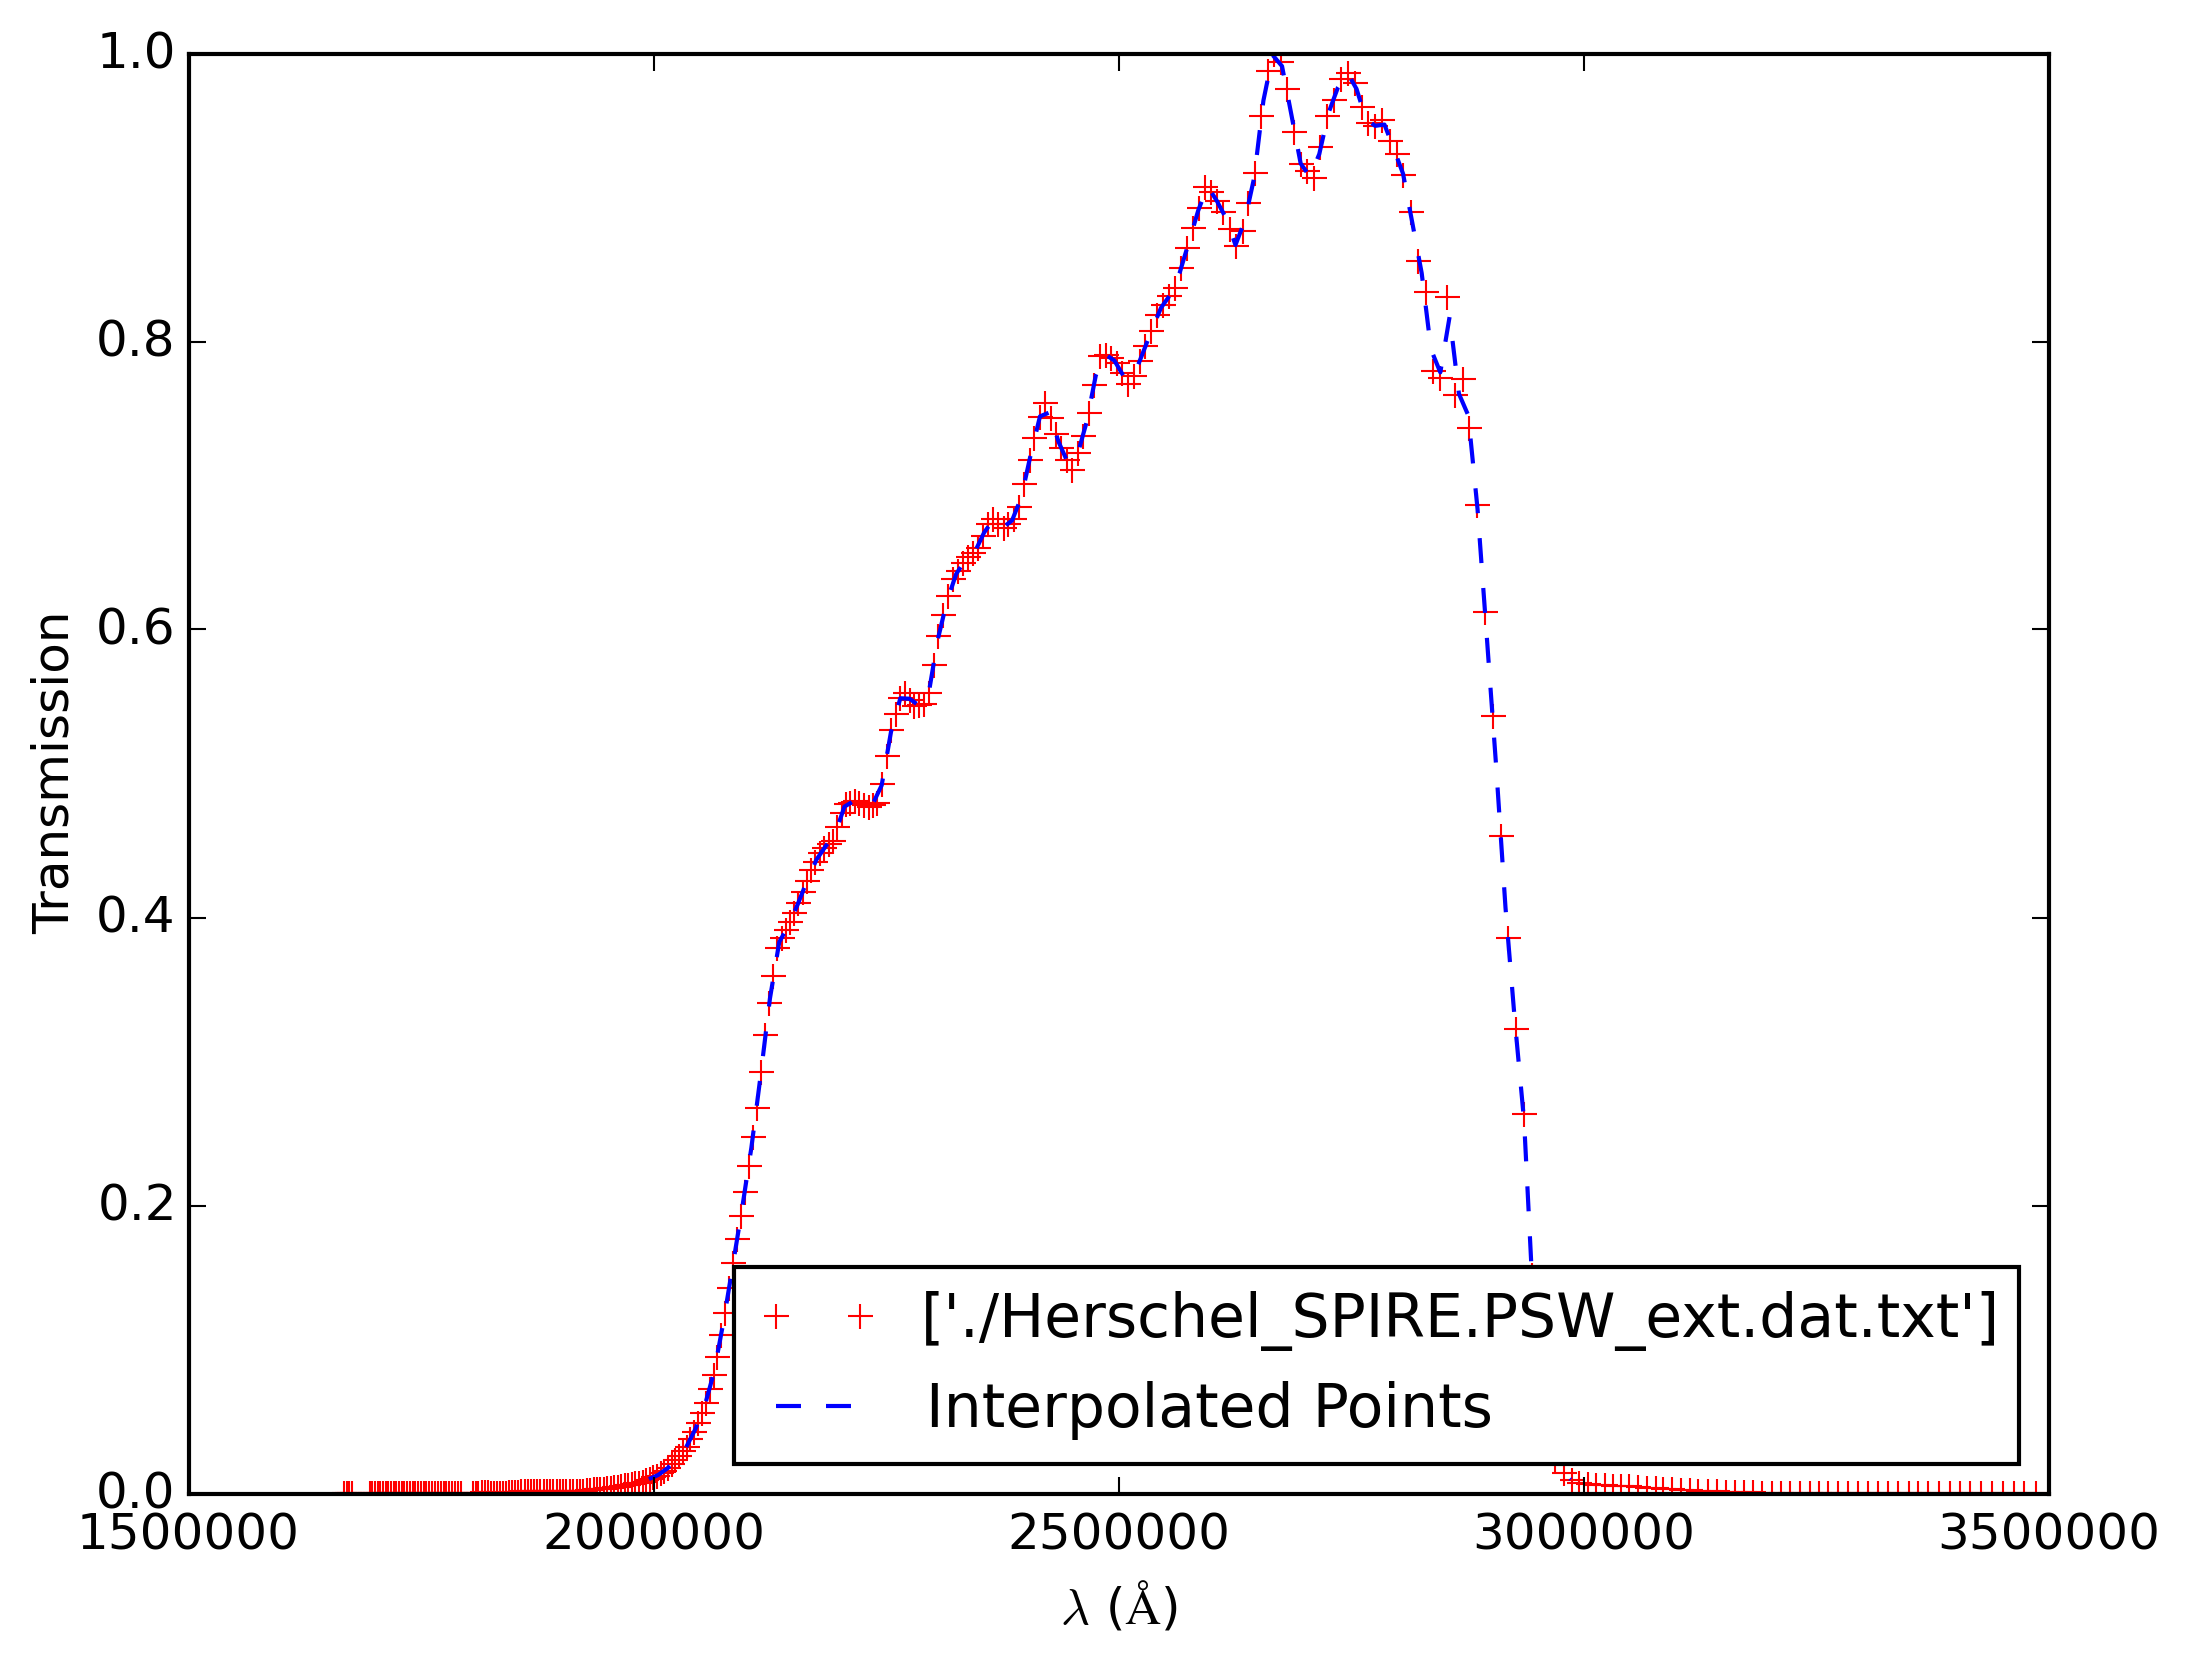
\includegraphics[width=\linewidth]{../img/interpolated_psw.png}
\caption{The transmission curve for the SPIRE PSW band.}\label{fig:psw}
\end{subfigure}

\begin{subfigure}[b]{.45\linewidth}
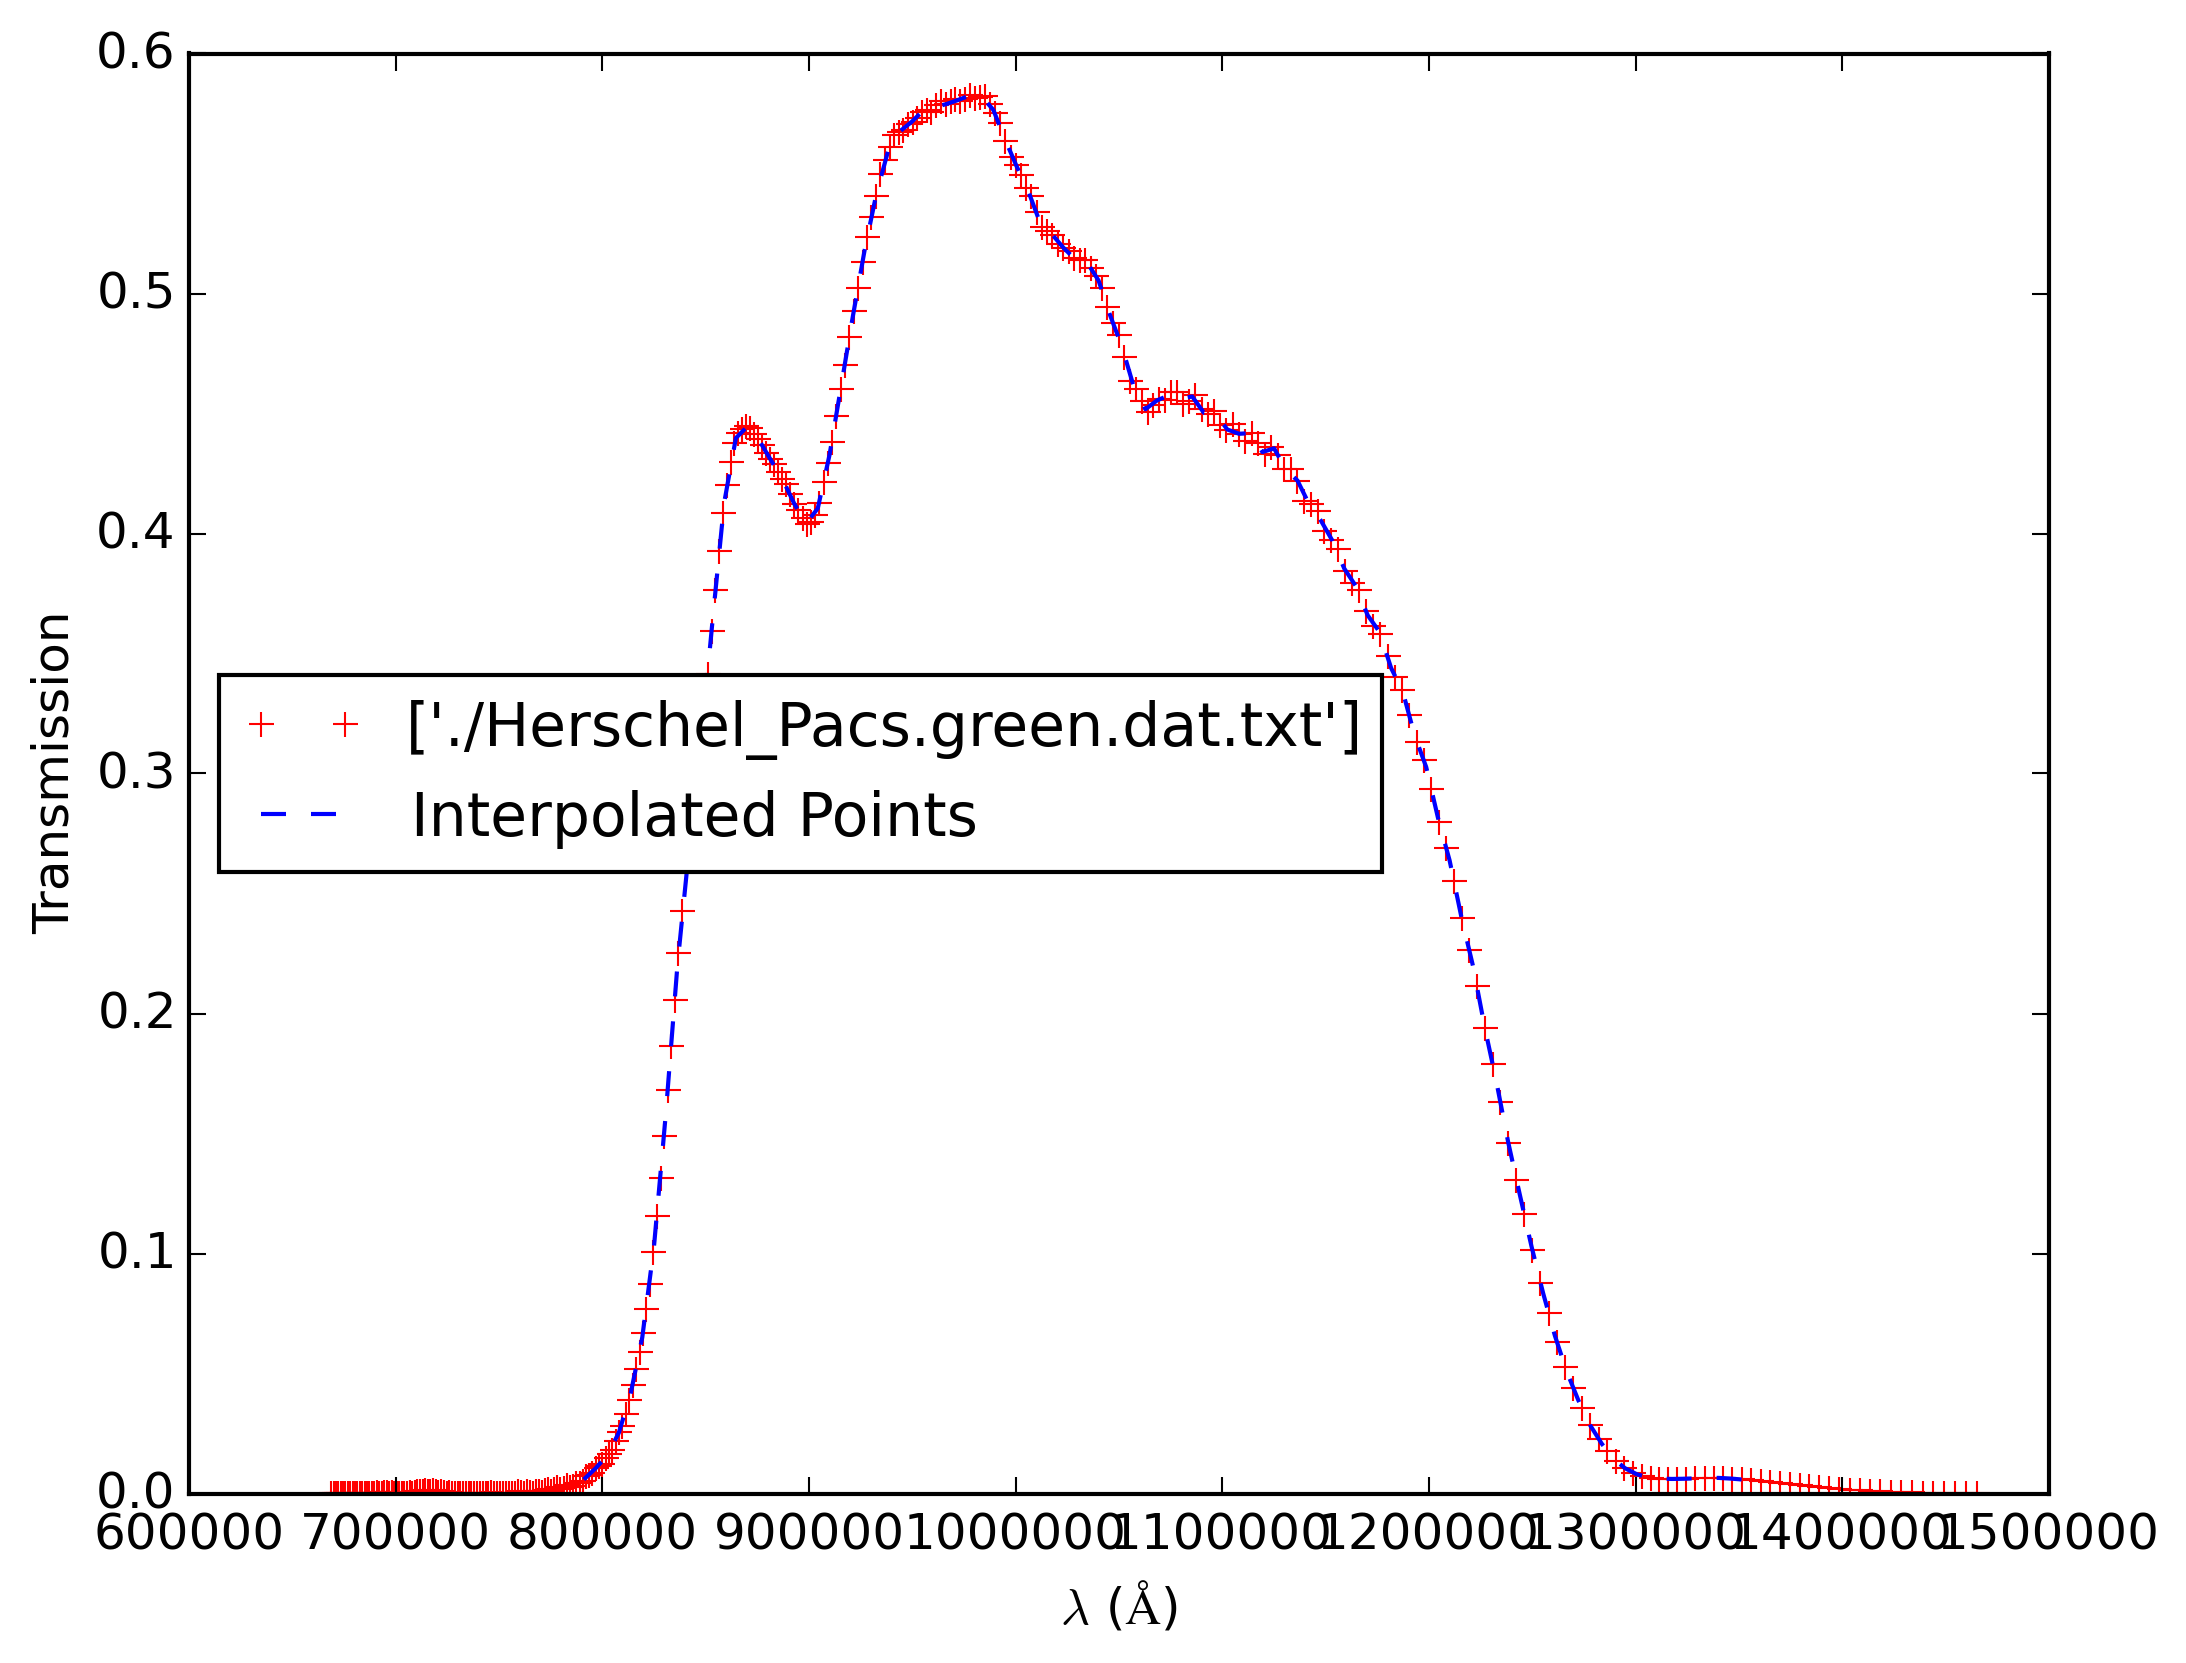
\includegraphics[width=\linewidth]{../img/interpolated_green.png}
\caption{The transmission curve for the PACS Green band.}\label{fig:green}
\end{subfigure}
\begin{subfigure}[b]{.45\linewidth}
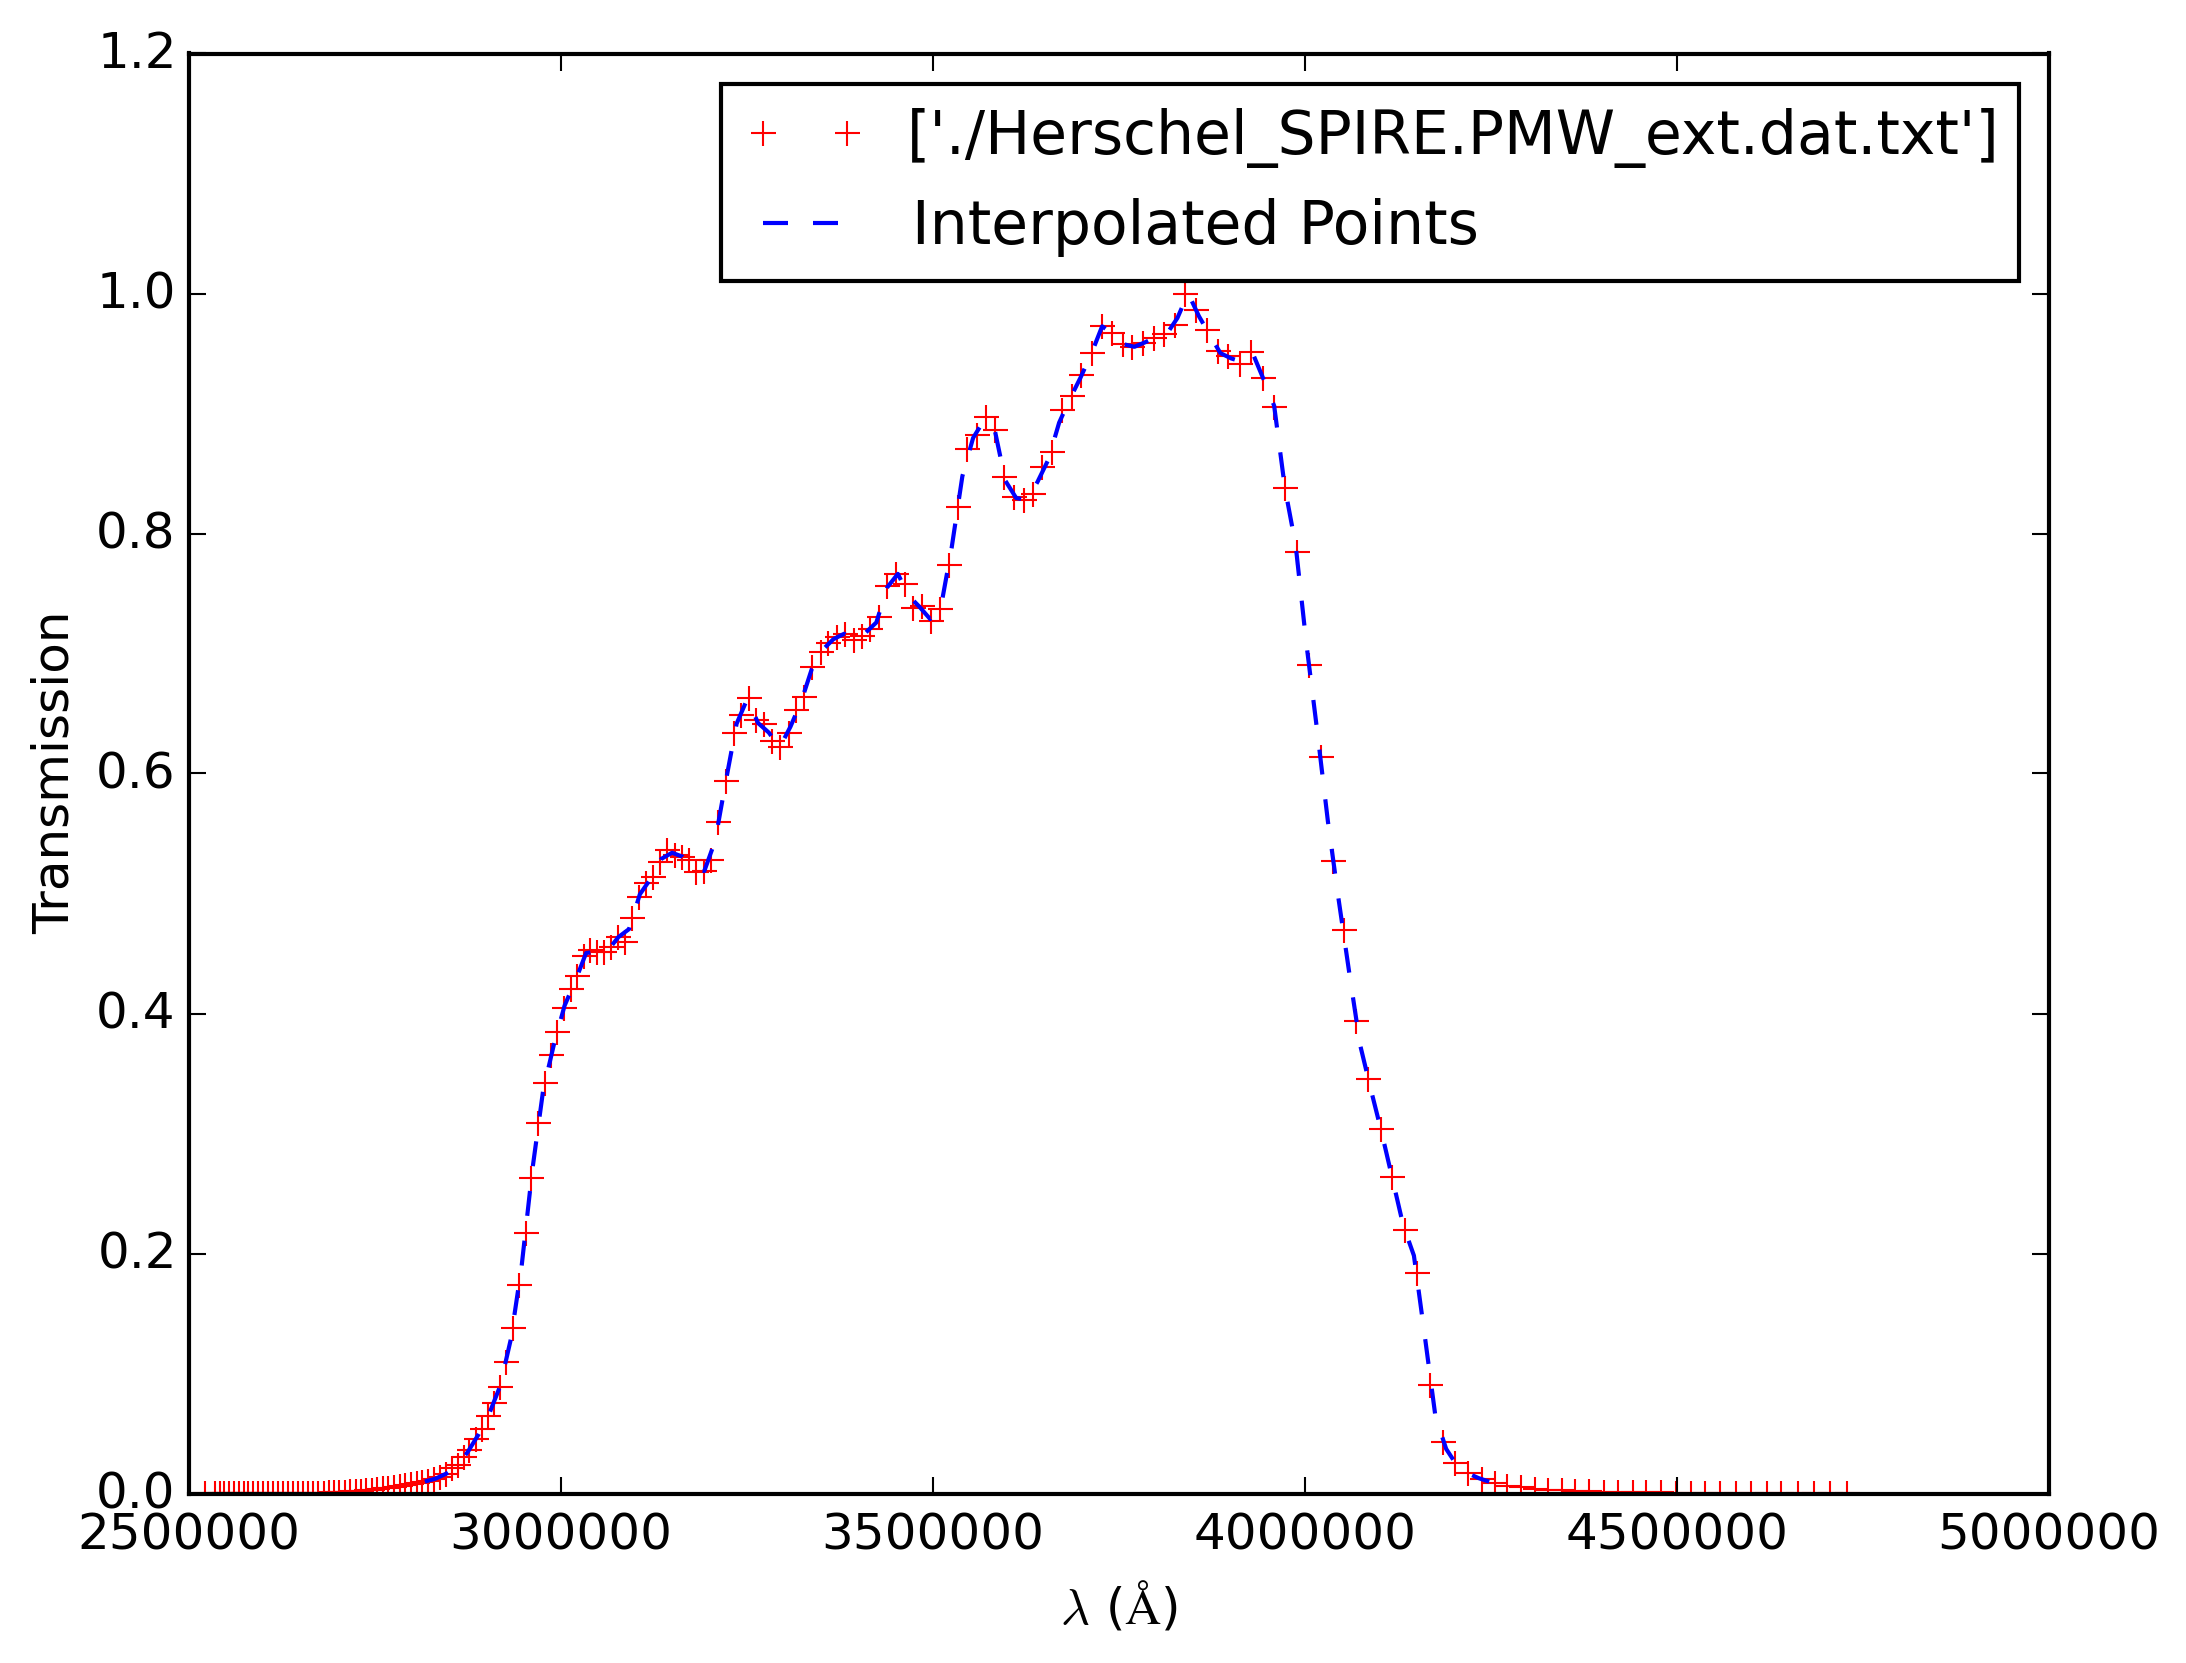
\includegraphics[width=\linewidth]{../img/interpolated_pmw.png}
\caption{The transmission curve for the SPIRE PMW band.}\label{fig:pmw}
\end{subfigure}

\begin{subfigure}[b]{.45\linewidth}
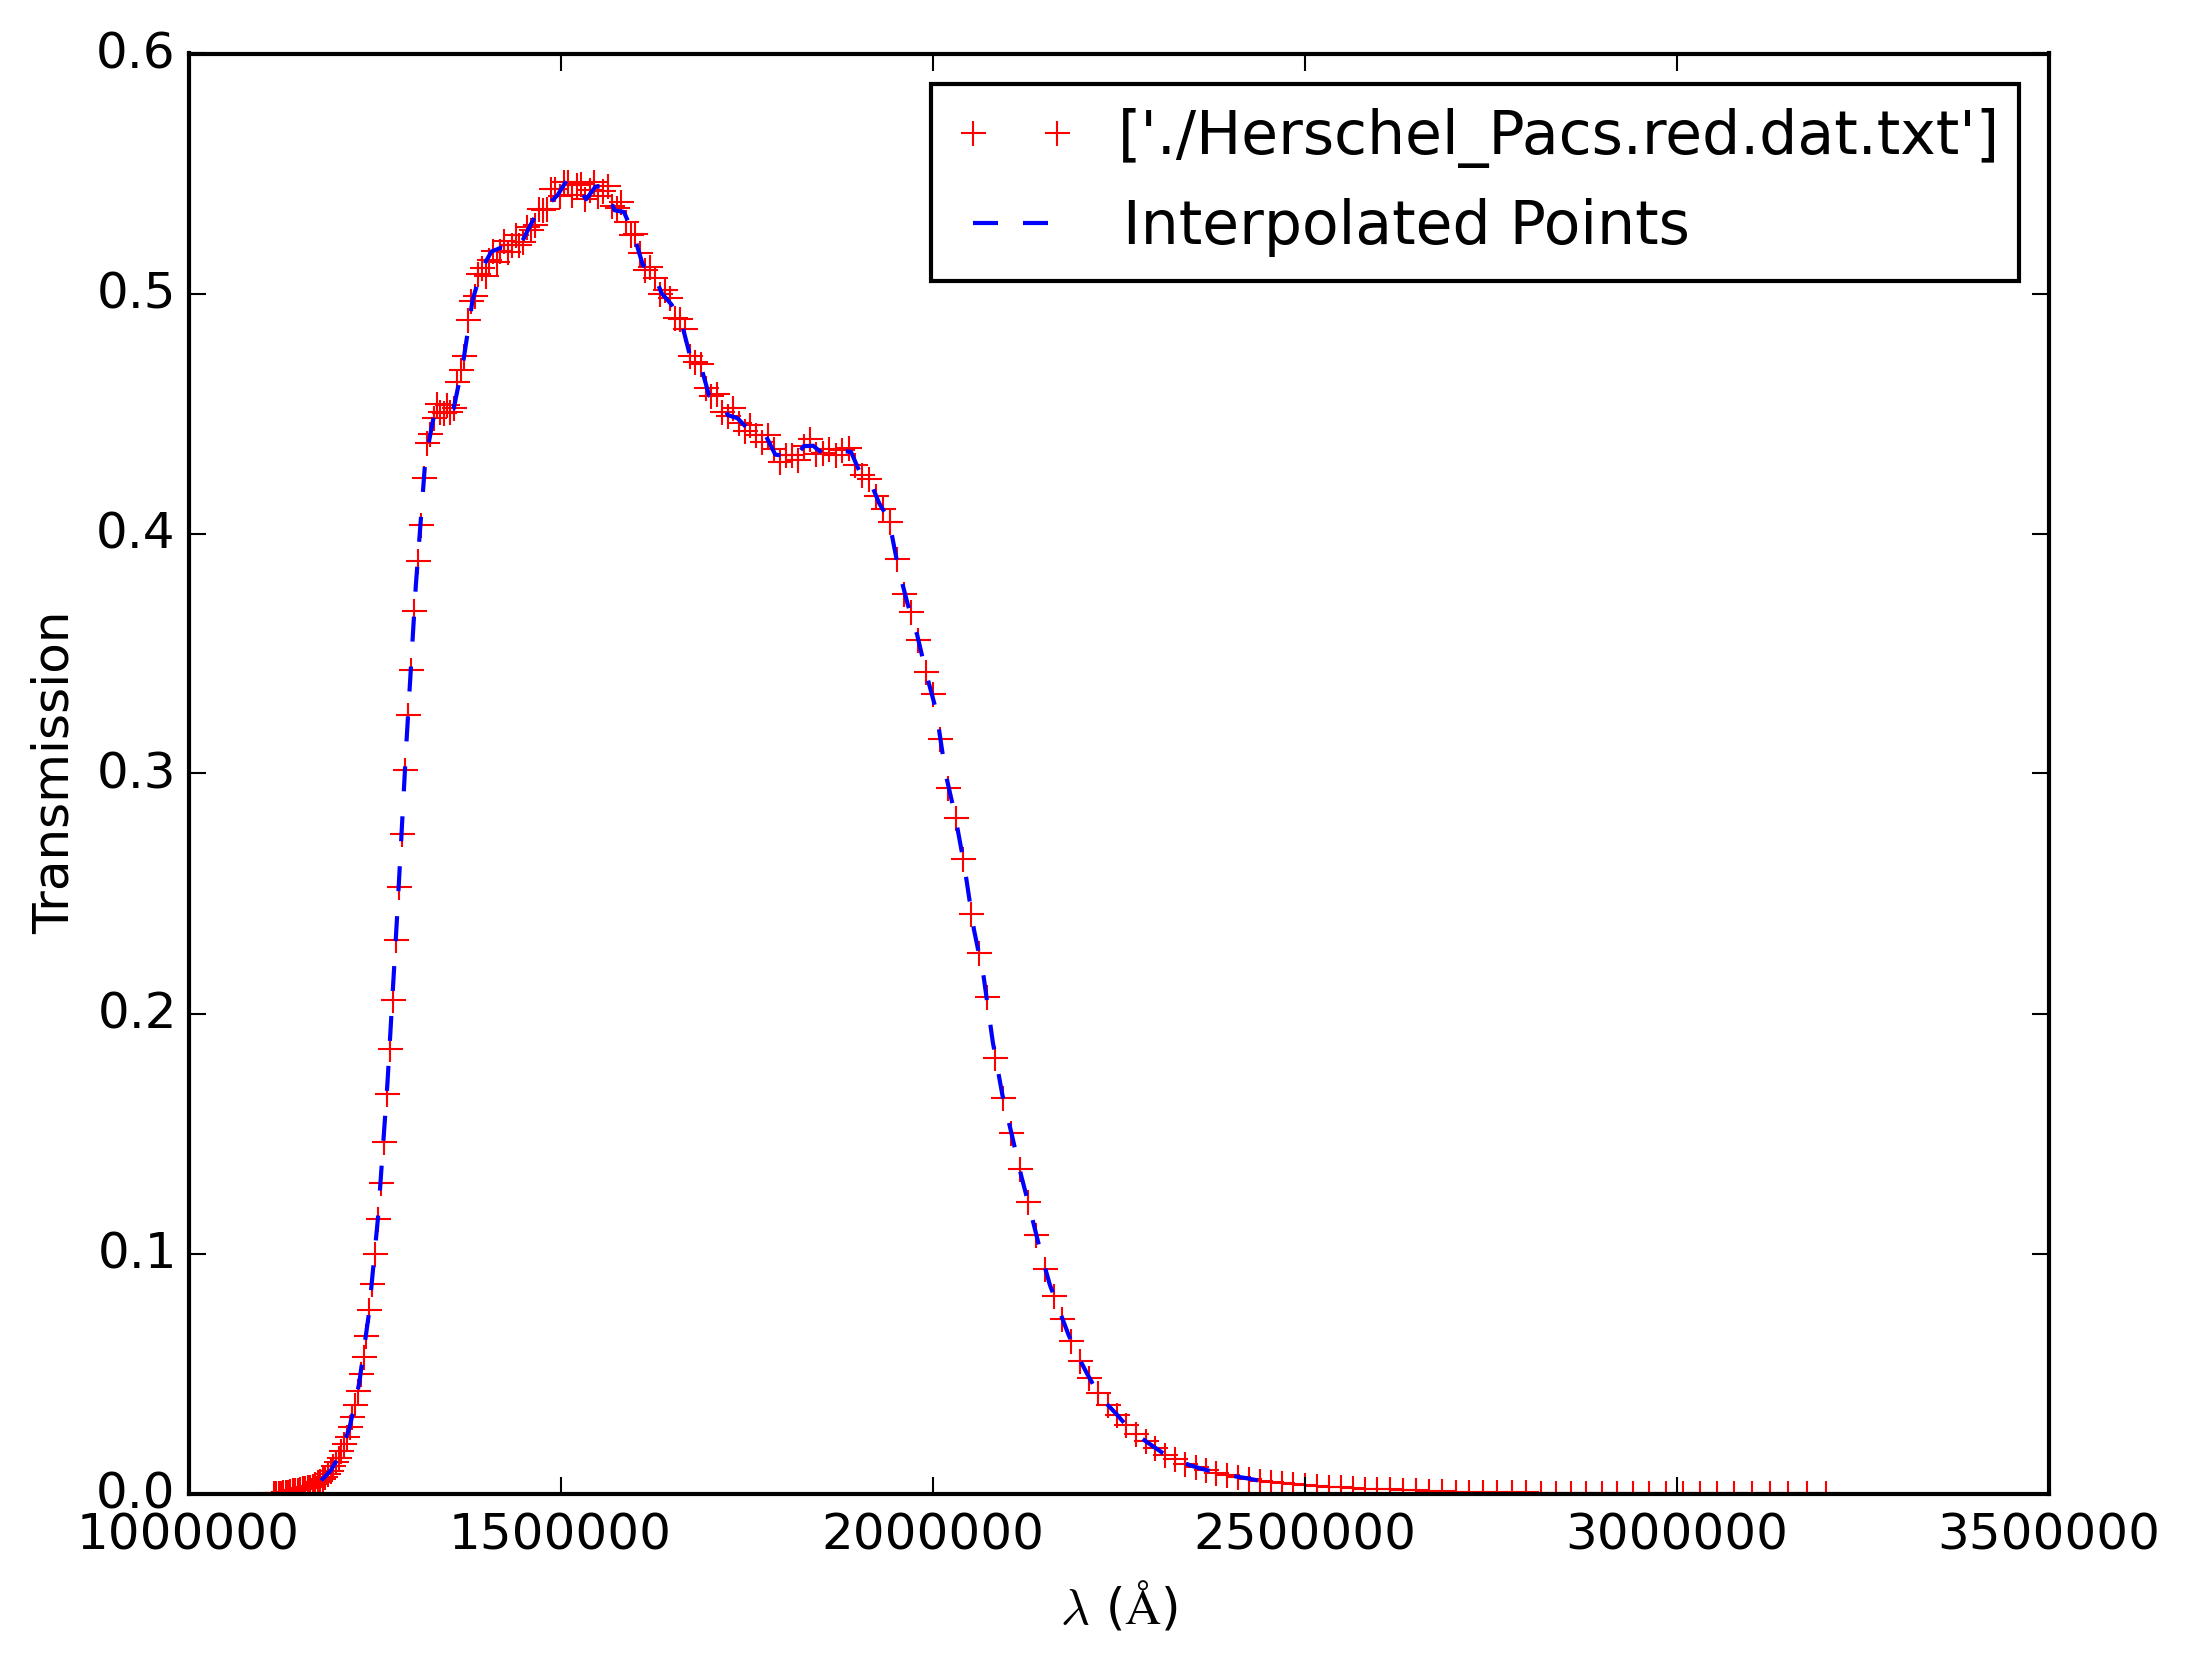
\includegraphics[width=\linewidth]{../img/interpolated_red.png}
\caption{The transmission curve for the PACS Red band.}\label{fig:red}
\end{subfigure}
\begin{subfigure}[b]{.45\linewidth}
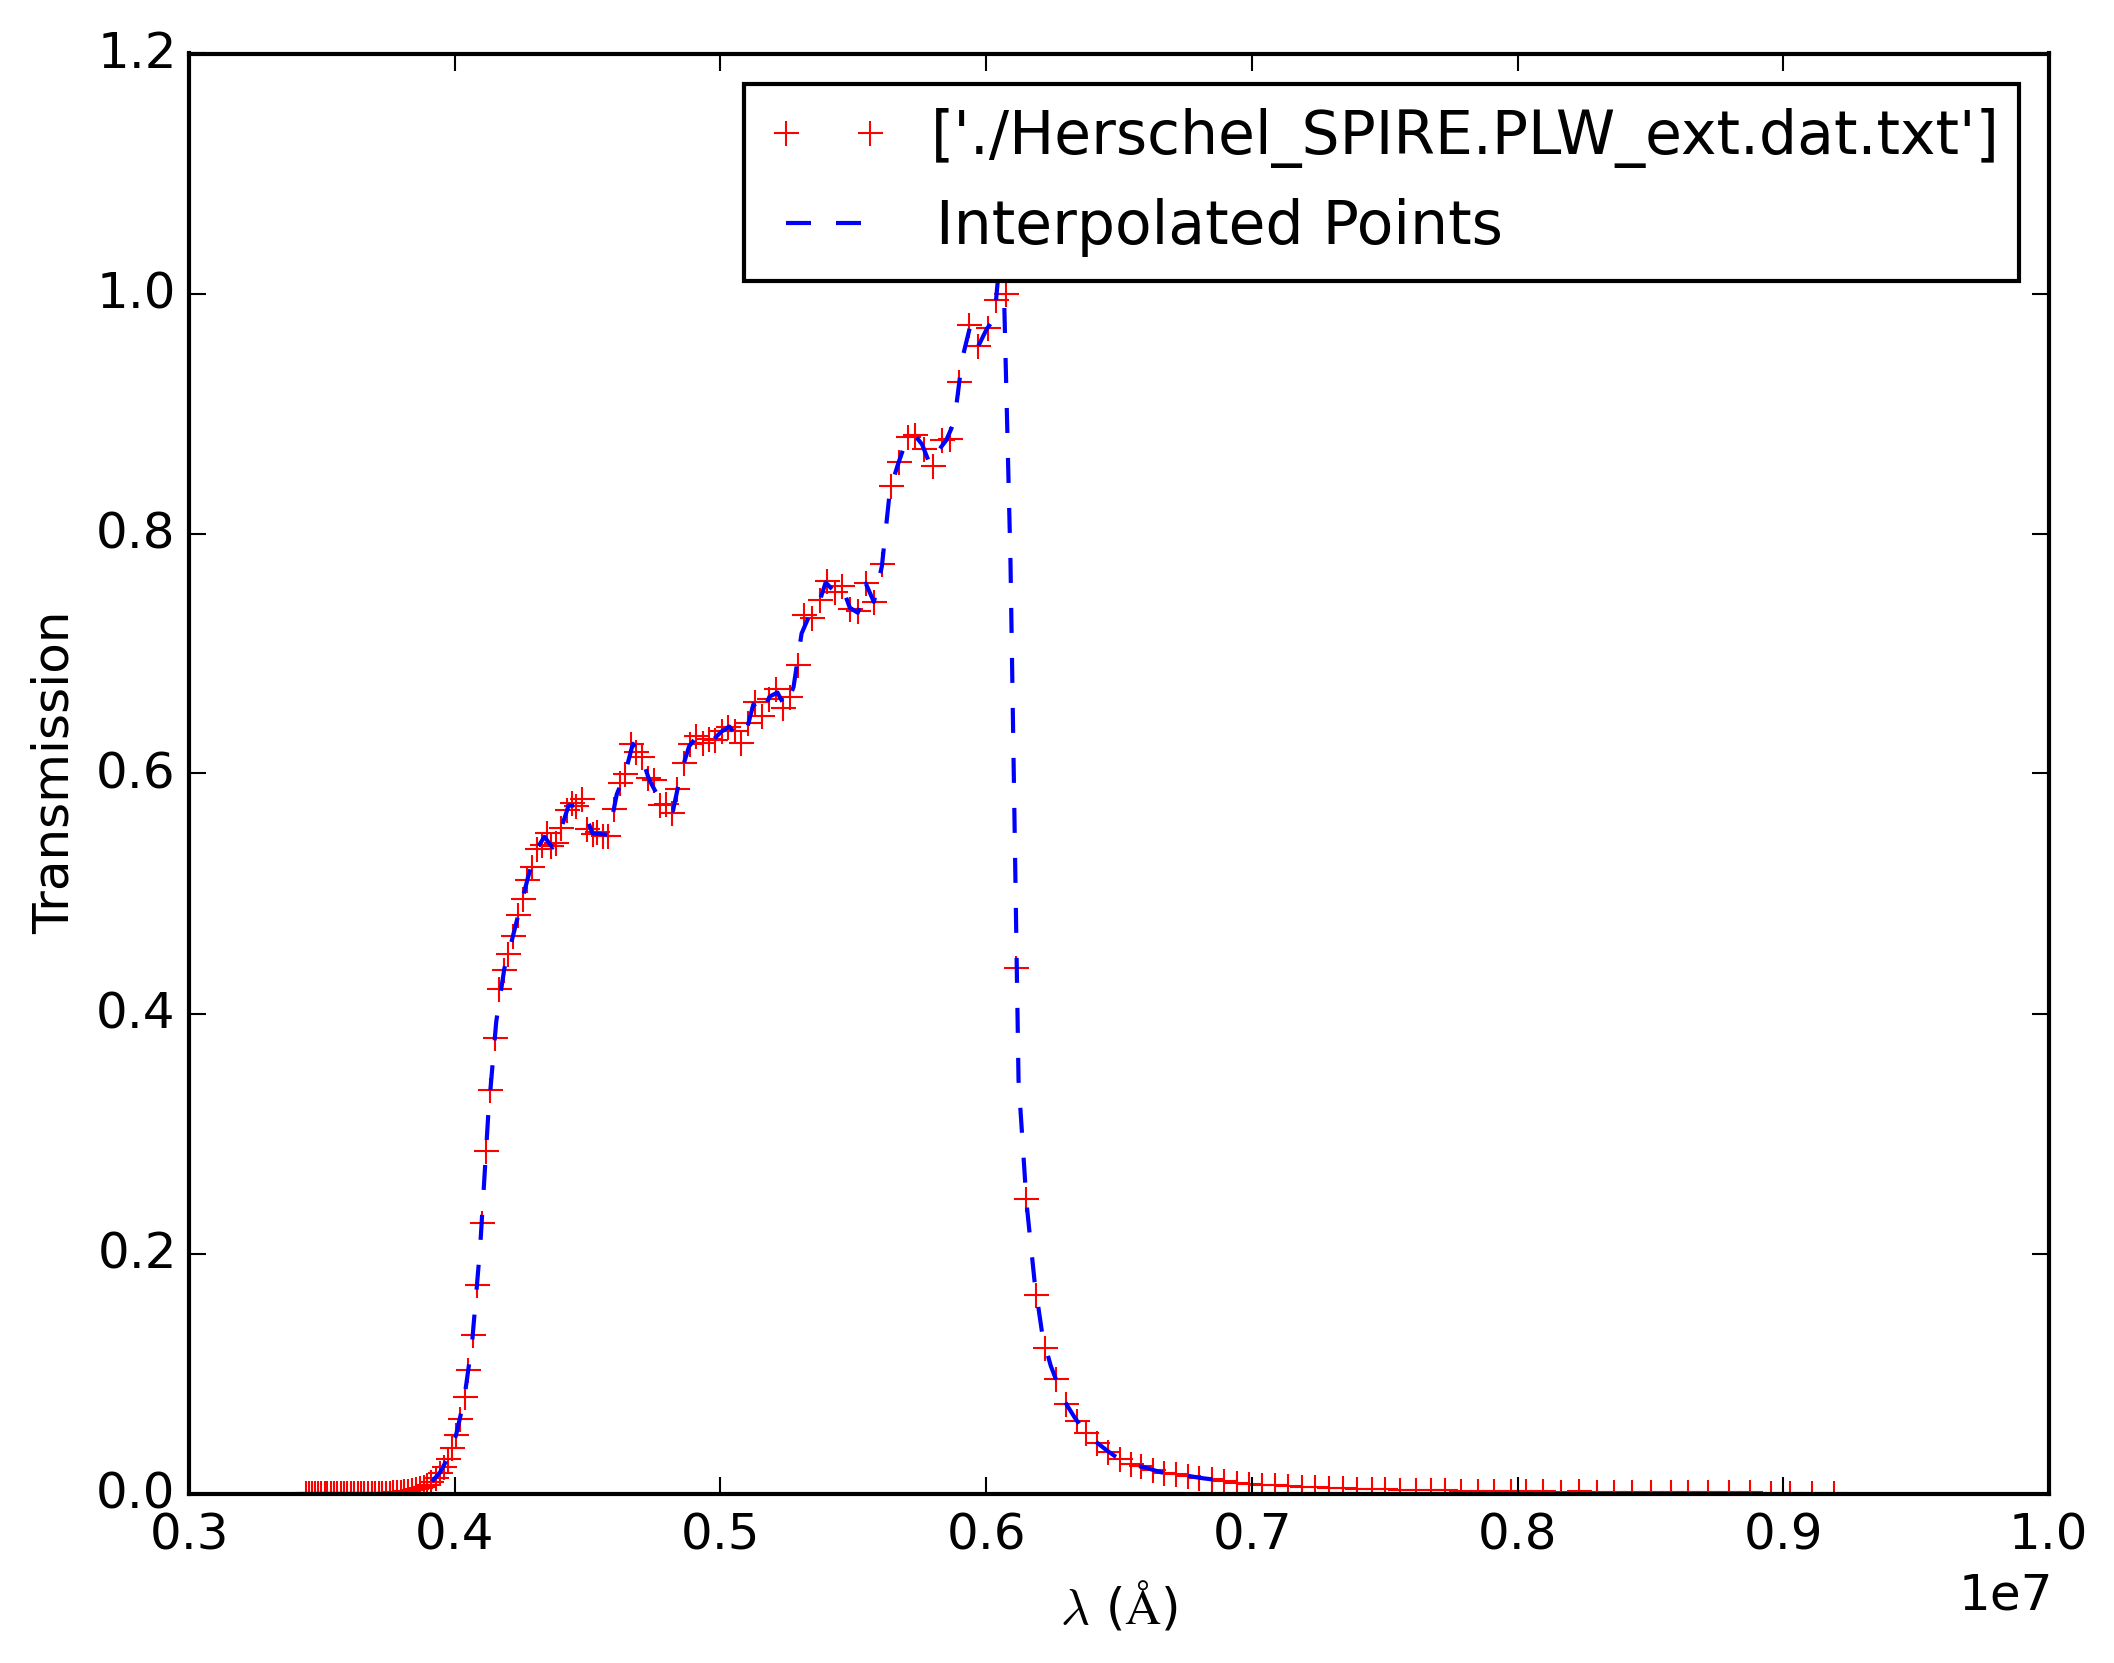
\includegraphics[width=\linewidth]{../img/interpolated_plw.png}
\caption{The transmission curve for the SPIRE PLW band.}\label{fig:plw}
\end{subfigure}
\caption{The transmission curves for each of the SPIRE PSW, PMW and PLW bands along with the PACS Blue, Red and Green bands.} \label{fig:transmission}
\end{figure}

Figure \ref{fig:transmission} illustrates this. The red $+$ datapoints indicate the original data supplied from \textcite{pass}, whilst the blue $--$ datapoints indicate the reconstructed, interpolated data. Figure \ref{fig:transmission} also illustrates that transmission is not constant across each filter. The interaction of the incoming waves with the filter material itself is frequency dependent, thus producing the curve.

To account for the transmission coefficients across the filter, multiplying each datapoint at a given frequency/wavelength by the transmission coefficient at that frequency/wavelength obtains the intensity of the photon after transmission. However the transmission data downloaded from \textcite{pass} is not linearly spaced, resulting in the transmission coefficients and freqencies not matching with those used in the simulation (specifically the data in \texttt{camera\_wavelength\_micron.inp} file). To account for this, cubic interpolation was used\footnote{Other routines to interpolate were available, however the cubic routine provided accurate results so alternatives were not explorered.} to produce a reconstruction of the original data with a user-defined number of points between upper and lower bounds. By choosing these upper and lower bounds to match the upper and lower bounds of \texttt{camera\_wavelength\_micron.inp} (with the same number of wavelength points) the transmission curve can be reconstructed to match the temporal data supplied to the simulation.

\subsection{Composite imaging} \label{comp}
In reality images are not taken at one discrete wavelength. Instead, images are a composite of wavelengths across a broad range defined by the telescope's filter. To illustrate, consider the SPIRE PSW band. As Table \ref{table:SPIRE-pass} illustrates, the PSW band is sensitive to wavelengths in the range $\SI{199.4540}{\micro\meter} --	\SI{298.5657}{\micro\meter}$. This means that an image using the PSW band is actually a composite image comprising a weighted average of the wavelengths imaged across such that the emergent image is effectively an image taken at the effective band wavelength. As a result of this, any transmission effects had to be accounted for in the image composition, such that Equation \ref{eq:trans} was used to construct the image intensities at each pixel.

\begin{equation}
  I_{xpix,ypix} = \frac{\sum_{i=0}^{npix} I_{xpix,ypix,\nu_i} T_{\nu_i}}{\sum_{i=0}^{npix} T_{\nu_i}}
  \label{eq:trans}
\end{equation}

$I_{xpix,ypix}$ is the pixel intensity whilst $I_{xpix,ypix,\nu_i}$ and $T_{\nu_i}$ are the intensity at $(xpix,ypix)$ and transmission coefficient at frequency $\nu_i$ respectively.  By performing the product of the intensity across all considered frequencies (i.e. $\nu_i$) at pixel $(xpix,ypix)$ with the transmission coefficent across all considered frequencies and normalising by dividing by the sum of all of the transmission coefficients in the dataset, the transmission weighted intensity can be computed at each pixel. Figure \ref{fig:no-trans} illustrates the output for a 3-dimensional isothermal cloud in RADMC-3D with perfect transmission (i.e. no transmission convolution). Figure \ref{fig:trans} illustrates the same image but with transmission being accounted for according to Equation \ref{eq:trans}. These images are computed in the Herschel PSW band.

\begin{figure}[!htb]
\minipage{0.48\textwidth}
  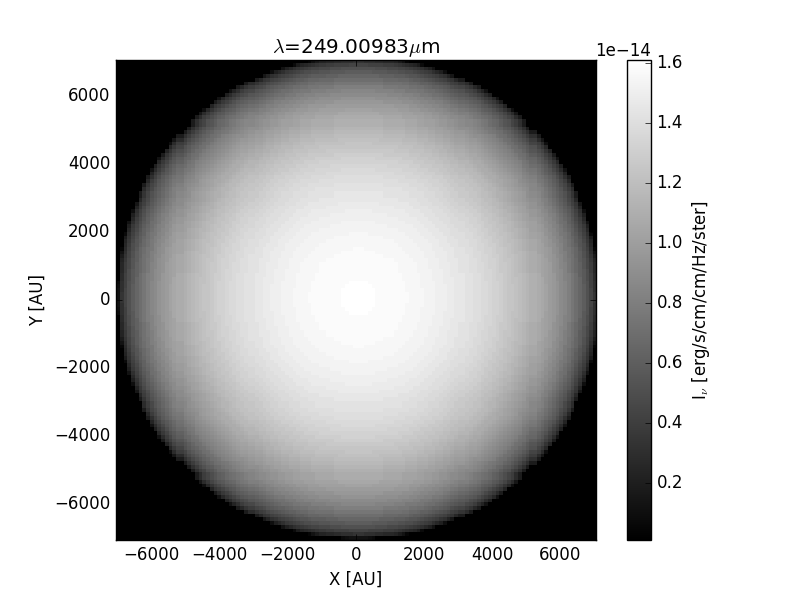
\includegraphics[width=\linewidth]{../img/figure_1_no_trans.png}
  \caption{The emergent image (before transmission effects) of a raytrace on a $1\/M_{Sun}$ spherical, 3D, isothermal ($T=10\/K$) cloud.}\label{fig:no-trans}
\endminipage\hfill
\minipage{0.48\textwidth}
  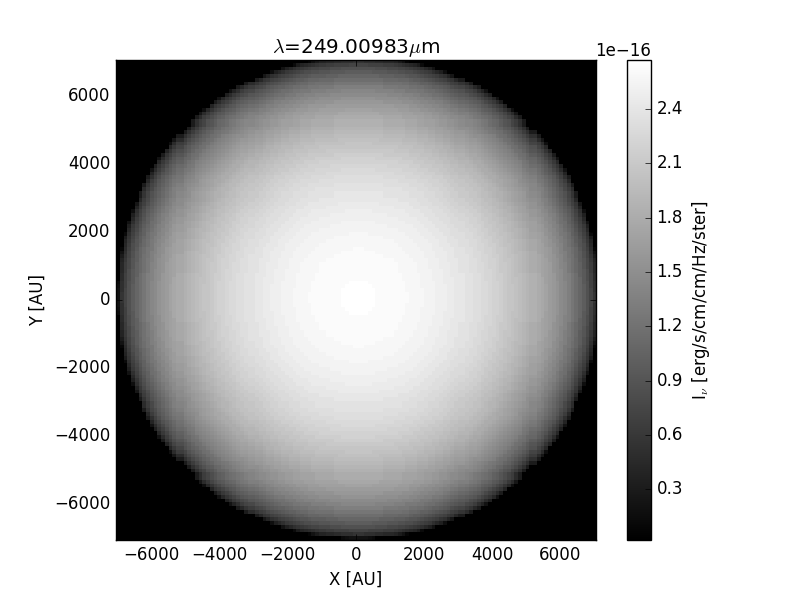
\includegraphics[width=\linewidth]{../img/figure_1.png}
  \caption{The emergent image (after transmission effects) of a raytrace on a $1\/M_{Sun}$ spherical, 3D, isothermal ($T=10\/K$) cloud.}\label{fig:trans}
\endminipage
\end{figure}

\section{Analysis routine}
The analysis routine used in the project can be split into 4 distinct stages:

\begin{enumerate}
  \item Use the discrete data from RADMC-3D images to produce SEDs
  \item Fit a modified blackbody to the SED on a pixel by pixel basis and utilise $\chi^{2}$ minimisation to derive the best fit $N$ and $T$
  \item Construct maps of $N$ and $T$ from both the $\chi^{2}$ derived values as well as the initial input values
  \item Extract prestellar core locations and masses from these maps using dendrogramic analysis
\end{enumerate}

\subsection{Spectral energy distributions (SEDs)}
Each individual source of flux has an energy distrubtion; that is, a function of how that point radiates as a function of frequency/wavelength. This function is continuous, and in the case of a blackbody source the SED can be described by the Planck function. Within the synthetic observations used in this project, each pixel within the computed image (rather than a discrete point) has an energy distribution. The SEDs in these cases are approximated using Equation \ref{eq:mbb-int} as opposed to the unaltered Planck function\footnote{Whilst the Planck function does not describe dust emission in this instance, a modified version of the Planck function does}. When imaging an object however this continuous SED is not observed. Instead, the telescope `sees` one, discrete intensity for each resolved point owing to the telescope's averaging over all observed frequencies as discussed in Section \ref{comp}. Figure \ref{fig:SED_ex} illustrates this.

\begin{figure}[h]{0.5\textwidth}
  \centering
  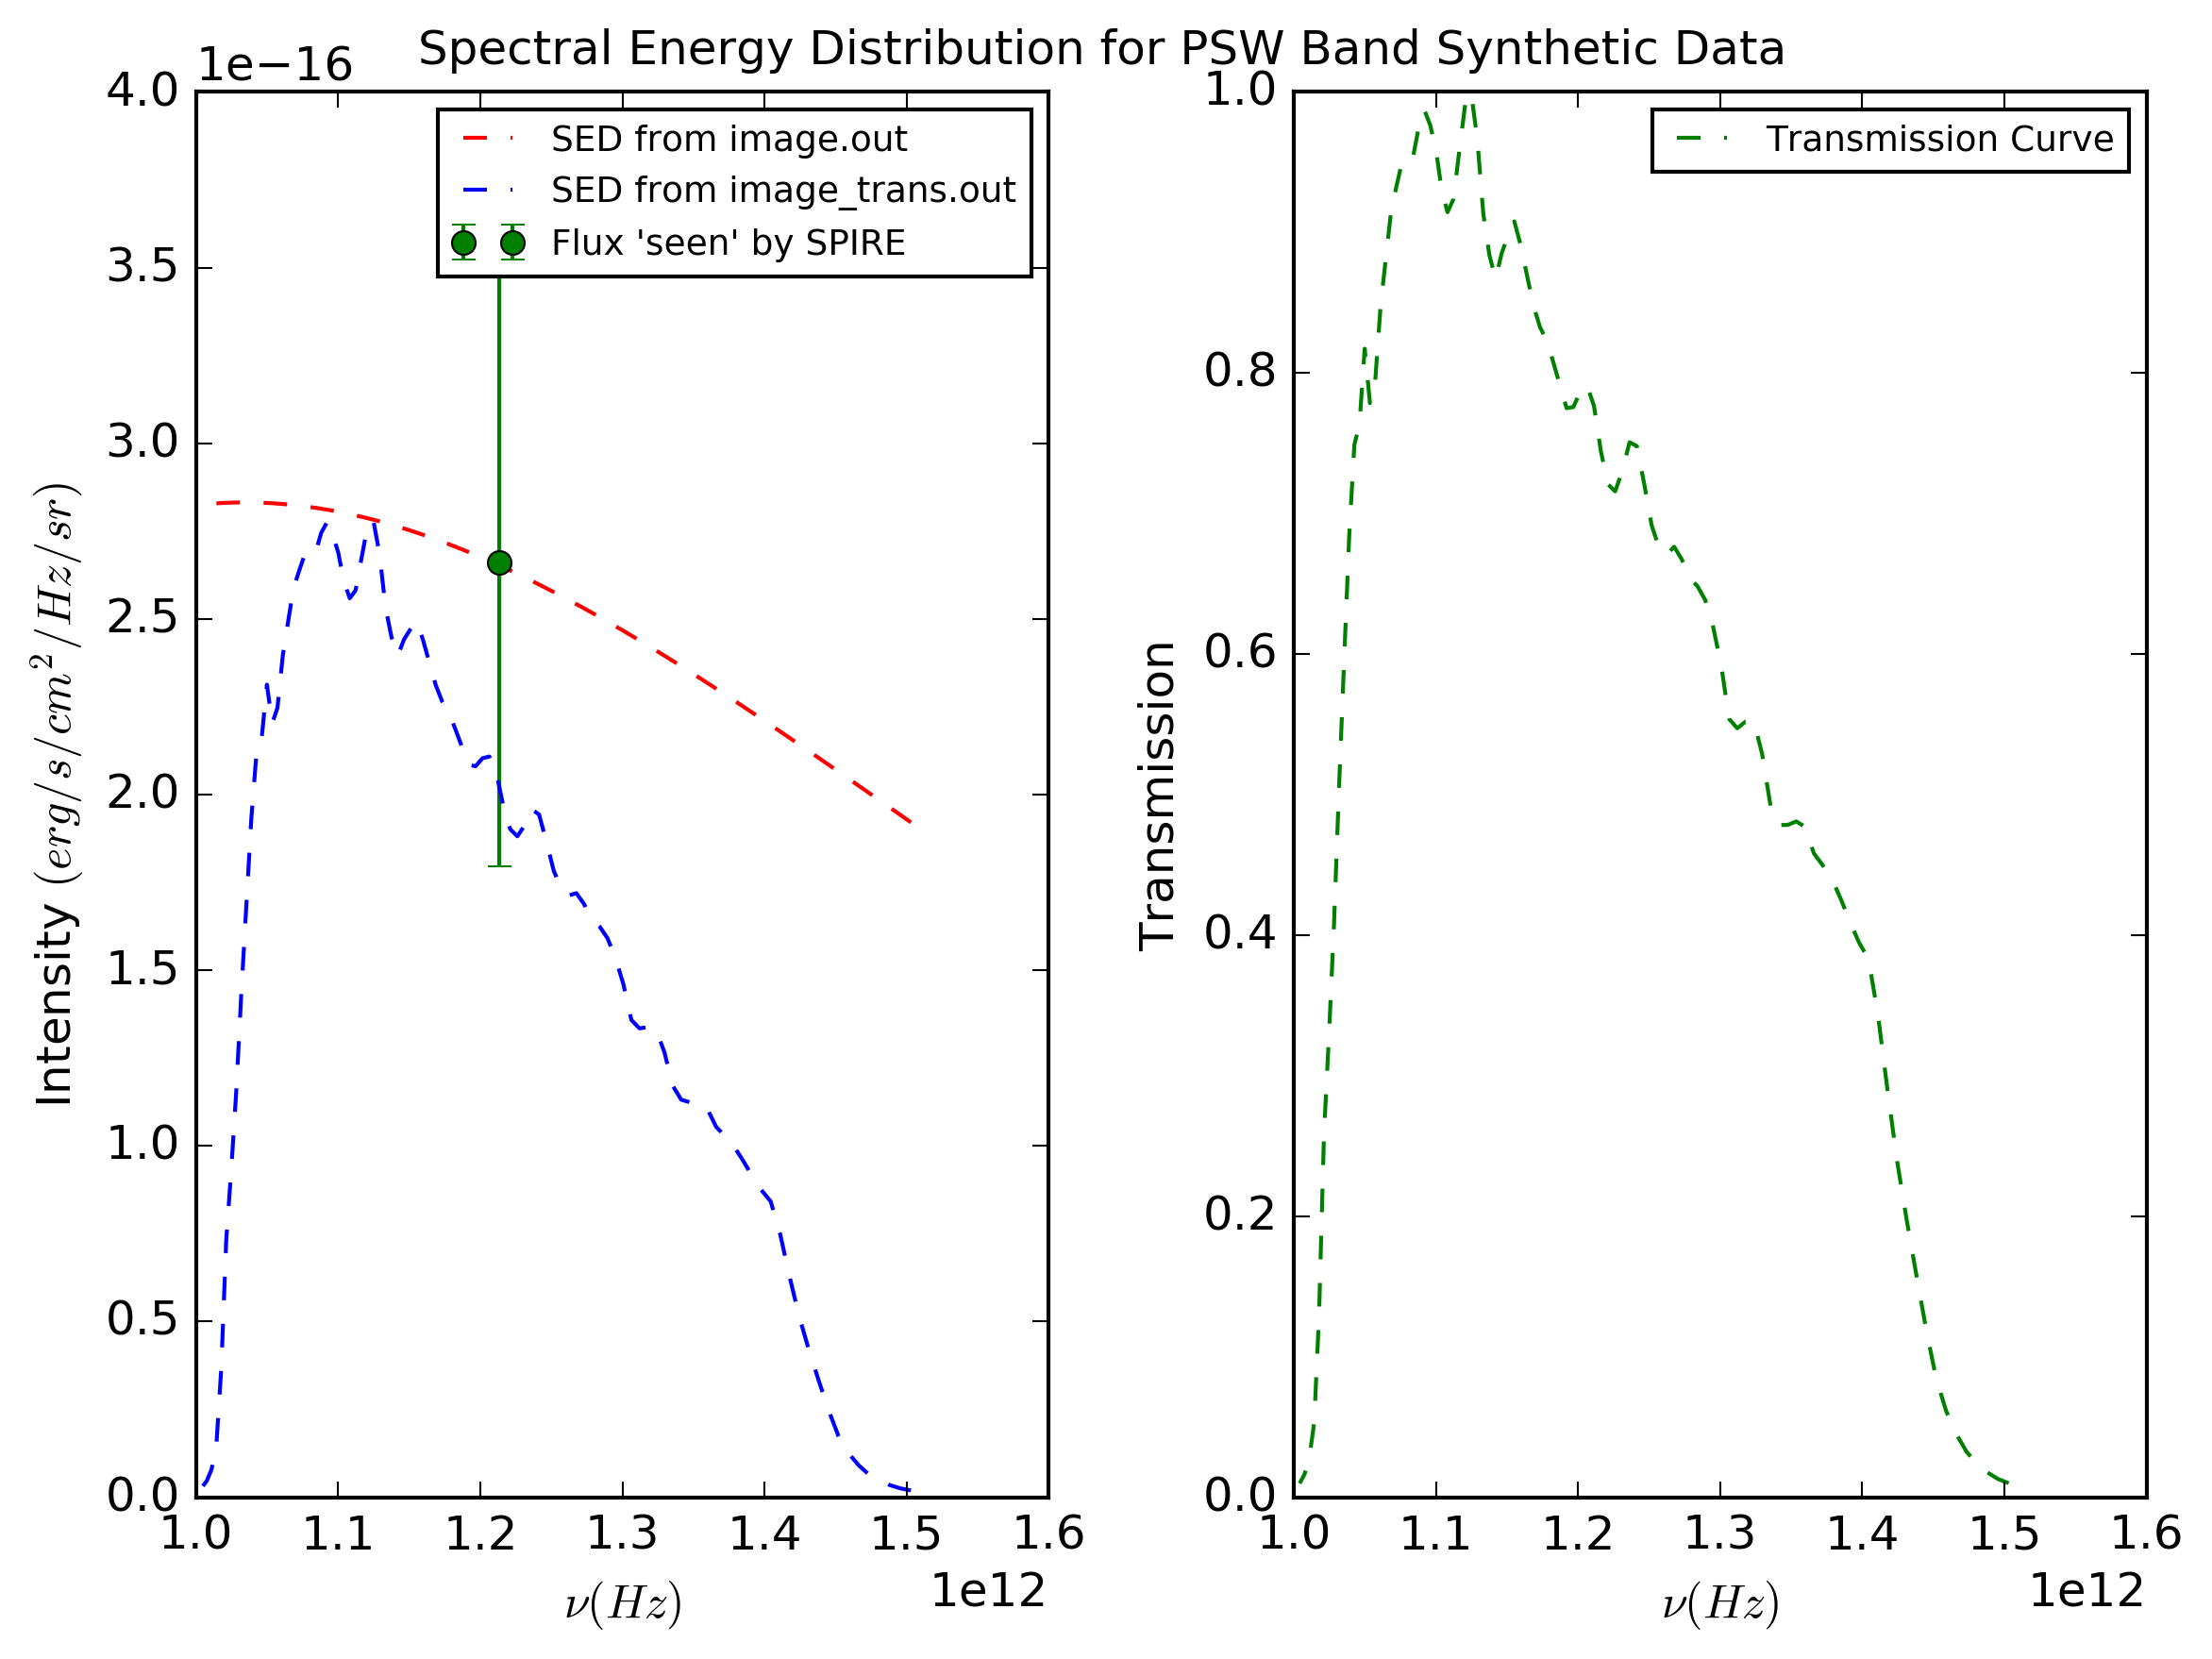
\includegraphics[scale=0.5]{../img/spectrum_psw_unweighted_v2}
  \caption[A figure showing the continuous SED sampled from \texttt{image\_trans.out}, along with the SED after convolving with the transmission curve (right hand panel). Also illustrated is the discrete point that Herschel would see were it to be observe this source in its PSW band.]{A figure showing the continuous SED sampled from \texttt{image\_trans.out}, along with the SED after convolving with the transmission curve (right hand panel). Also illustrated is the discrete point that Herschel would see were it to be observe this source in its PSW band.}
  \label{fig:SED_ex}
\end{figure}

Figure \ref{fig:SED_ex} shows the SED for the central pixel (0,0) of Figure \ref{fig:trans} imaged in the PSW band. This SED is sampled directly from \texttt{image\_trans.out} by taking the intensity of the pixel (in this case the (0,0) pixel) at each discrete frequency/wavelength considered. Plotting the intensity as a function of frequency produces the red continua in the left hand panel. Convolving the theoretical SED with the transmission curve for the band imaged in produces the SED that falls on to Herschel's filter. This is displayed as the blue curve in the left hand panel. The green point represents the intensity incident upon the detector, as determined by Equation \ref{eq:seen}.

\begin{equation}
  I_{pix} = \frac{\sum_{\nu} I_{pix,\nu}}{\sum_{\nu} T_{\nu}}
  \label{eq:seen}
\end{equation}

$I_{s}$ is the averaged intensity as measured by Herschel, whilst $I_{pix,\nu}$ is the image intensity at frequency $\nu$ and $T_{\nu}$ is the transmission coefficient at frequency $\nu$.

Repeating this procedure for each band on board SPIRE and PACS allows a dataset of points to be built up as a function of frequency. This dataset then acts as an `expected` dataset that is described by Equation \ref{eq:mbb-int}. As a direct result of this, fitting Equation \ref{eq:mbb-int} to the `expected` dataset using a $\chi^{2}$ minimisation routine allowed the 2 fit parameters, $N$ and $T$ to be determined.

\subsection{Parameter estimation}
A $\chi^{2}$ minimisation test is a statistical test to assess the `goodness-of-fit` between observed data and a theoretical model. The value of $\chi^{2}$ is determined via Equation \ref{eq:chi} \parencite{error}.

\begin{equation}
  \chi^{2} = \sum_{i}\Bigg (\frac{O_{i}-E_{i}}{\sigma_{i}} \Bigg )^{2}
   \label{eq:chi}
\end{equation}

$O_{i}$ is an observed point, and $E_{i}$ is the expected point. $\sigma_{i}$ is the standard deviation of $O_{i}$. If $O_{i}$ is a given dataset and $E_{i}$ is the model that is expected to fit that dataset, then $\chi^{2}$ is therefore a measure of how close that model fits the data within one standard deviation.

By applying this $\chi^{2}$ test to assess how well the modified blackbody given in Equation \ref{eq:mbb-int} fits the observed data, recovery of both $N$ and $T$ is possible. We perform this on a pixel by pixel basis such that $N$ and $T$ can be determined for each pixel in the data. The observed points used here, $O_{i}$, are 6 discrete points, however the function being fitted for, $E_{i}$, is continuous across a frequency range $\nu$. As the continua produced by the model is evaluated over the same frequency range $\nu$, the index of each of the observed points in $\nu$ is also the index of the intensity in the continua. By then evaluating Equation \ref{eq:mbb-int} using given values of $N$ and $T$ the expected continua can be determined. Subsequently pulling out the points within this continua that match the indices from the discrete points and applying the
$\chi^{2}$ test given in Equation \ref{eq:chi} allowed the `goodness-of-fit` of that given curve to the observed data to be evaluated. Systematically repeating this process across all values of $N$ and $T$ produces a $\chi^{2}$ landscape. The minimum value of $\chi^{2}$ within this landscape corresponds to the theoretical best fit; by locating the values of $N$ and $T$ that produced this minimised curve, the best fit parameters can be determined. This procedure was then applied to the next pixel in the image until all pixels had been analysed and their best fit parameters estimated, therefore producing best fit values of $N$ and $T$ at each pixel.

The $\chi^{2}$ fitting routine is also the major source of error in $N$ and $T$ estimation and so these errors were accounted for by analysing the $\Delta \chi^{2}$ landscape. By expressing $\chi^{2}$ as $\chi^{2} = \chi^{2}_{min} + \Delta \chi^{2}$, a region around $\chi^{2}_{min}$ can be isolated by drawing lines of constant $\chi^{2}$ characterised by $\Delta \chi^{2}$. These regions contain a varying percentage of the fit parameters depending upon the value of $\Delta \chi^{2}$ described in Table \ref{table:delta}.

\begin{table}[]
\centering
\begin{tabular}{|c|c|cccc}
  \hline
  \textit{\textbf{$k -\sigma$}} & \textit{\textbf{$P$}} & \multicolumn{1}{c|}{\textit{\textbf{$M = 1$}}} & \multicolumn{1}{c|}{\textit{\textbf{$M = 2$}}} & \multicolumn{1}{c|}{\textit{\textbf{$M = 3$}}} & \multicolumn{1}{c|}{\textit{\textbf{$M = 4$}}} \\ \hline
  $1 -\sigma$                   & 68\%                  & 1                                              & \textbf{2.30}                                           & 3.53                                           & 4.72                                           \\ \cline{1-2}
  $2 -\sigma$                   & 95.4\%                & 4                                              & \textbf{6.17}                                           & 8.02                                           & 9.70                                           \\ \cline{1-2}
  $3 -\sigma$                   & 99.73\%               & 9                                              & \textbf{11.8}                                           & 14.2                                           & 16.3                                           \\ \cline{1-2}
  \end{tabular}
  \caption{A table showing the values of $\Delta \chi^{2}$ for fit parameters in varying $M$ dimensions. Bold parameters are those used in this study \parencite{recipes}}
  \label{table:delta}
\end{table}

This project required 2 fit parameters in $N$ and $T$. The values of $\Delta \chi^{2}$ used in this study are shown in bold in Table \ref{table:delta}. The corresponding confidence interval is shown in the $P$ column. All errors quoted hereafter correspond to the $1 - \sigma$ interval.

\section{Image construction} \label{sec:imag_construct}

\subsection{2D Maps of $N$ and $T$}
The result of the $\chi^{2}$ minimisation is a best fit value of $N$ and $T$ at each pixel. 2-dimensional heat maps can be plotted that graphically illustrate the recovered values. This process is also repeated for the reconstructed values of $N$ and $T$ from the initial input data files \texttt{dust\_density.inp} and \texttt{dust\_temperature.dat} by Equations \ref{eq:N_data} and \ref{eq:T_data}.

\noindent\begin{minipage}{.5\linewidth}
\begin{equation}
  N_{col} = \sum{\frac{\rho_{d}d_{cell}}{\mu m_{p}}}
  \label{eq:N_data}
\end{equation}
\end{minipage}%
\begin{minipage}{.5\linewidth}
\begin{equation}
  T_{pix} = \frac{\sum_{i} T_{i} \rho_{i}}{\sum_{i} \rho_{i}}
  \label{eq:T_data}
\end{equation}
\end{minipage}

Within Equation \ref{eq:N_data}, $N_{col}$ is the column density of the pixel, $\rho_{d}$ is the dust density at that pixel, $\mu$ is the mean molecular weight, $\mu$ is the mean molecular weight, $m_{p}$ is the mass of the proton and $d_{cell}$ is the size of the RADMC-3D cell in the Z dimension. This is summed over the pixels along the line of sight.

Within Equation \ref{eq:T_data}, $T_{pix}$ is the temperature of the pixel, $T_{i}$ and $\rho_{i}$ are the column-weighted temperature and dust density at $ith$ pixel along the line of sight. The RADMC-3D temperature inputs at each cell are largely independent of the density at that cell, however when observed the varying column density along the line of sight causes the temperature observed to vary as well. This is not the case at the source of emission, and Equation \ref{eq:T_data} accounts for that such that it determines the temperature of the dust as it was emitted and not as it was observed. It is this column-weighted temperature that the $\chi^{2}$ routine fits for.

The temperature variation along the line of sight, $\sigma_{T_{N}}^{2}$ can also be computed using Equation \ref{eq:los}.

\begin{equation}
  \sigma_{T_{N}}^{2} = \frac{\sum{(T_{data}-T_{col})^{2}}N_{inp}}{\sum{N_{inp}}}
   \label{eq:los}
\end{equation}

$T_{data}$ is the initial data input temperature, $T_{col}$ is the data derived temperature whilst $N_{inp}$ is the data derived $N$.

Computing maps of $N$ and $T$ from both the $\chi^{2}$ recovered values as well as the theoretical predictions based on Equations \ref{eq:N_data} and \ref{eq:T_data} from the input data allows both data to be compared and constrasted.

Along with maps of $N$ and $T$, we also produce probability density functions (PDFs). These allow the distribution of $N$ and $T$ within a given map to be analysed. It also allows a further measure of comparison between $\chi^{2}$ and theoretical predictions.

\subsection{Dendrogram analysis}
As Section \ref{sec:conditions} stated, molecular clouds have a hierarchical structure according to their fragmentation and collapse. This produces a complex structure within the cloud, often with regions of having substructure according to any hierarchical fragmentation that it may undergo during collapse. This structure can be analysed using maps of $N$ but it can also be probed with dendrogramic analysis. All dendrograms within the study are plotted using \texttt{astrodendro} \parencite{astrodendro}.

A dendrogram is a graphical representation that shows the relationship between individual datapoints in a set by way of a tree diagram. An example dendrogram is shown Figure \ref{fig:dendrogram}.

\begin{figure}[h]
  \centering
  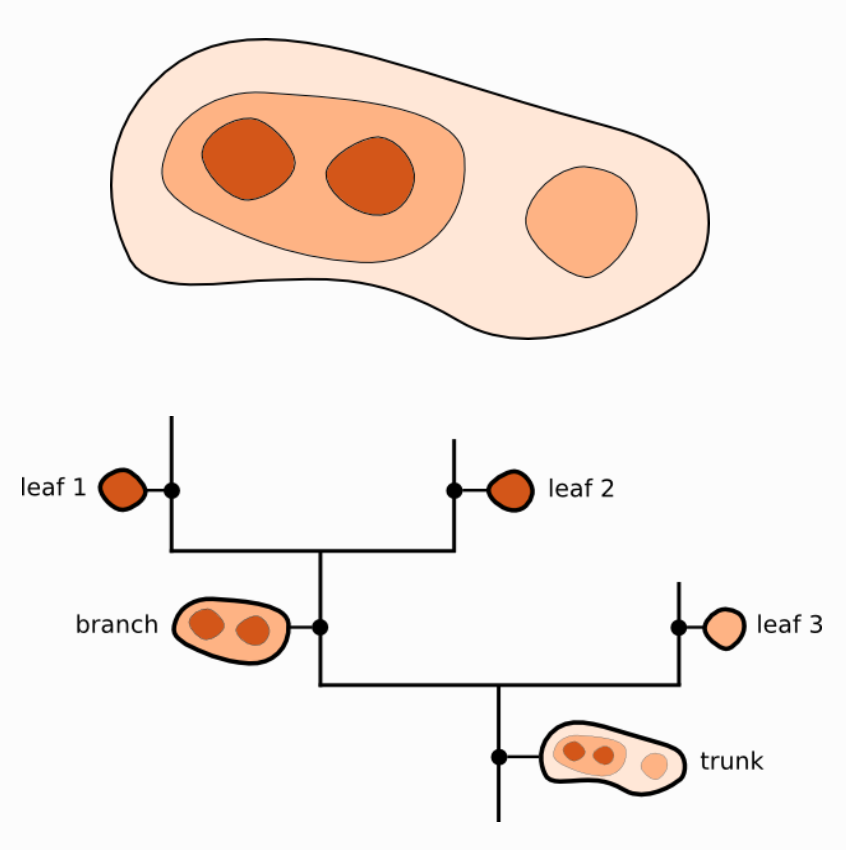
\includegraphics[scale=0.5]{../img/dendrogram}
  \caption[An idealised molecular cloud containing some substructure defined by sequentially darker regions. Below, the dendrogramic representation of the cloud \parencite{dendrogramimg}.]{An idealised molecular cloud containing some substructure defined by sequentially darker regions. Below, the dendrogramic representation of the cloud \parencite{dendrogramimg}.} \label{fig:dendrogram}
\end{figure}

As Figure \ref{fig:dendrogram} shows, the dendrogram highlights the relationships between areas in the image. If Figure \ref{fig:dendrogram} represents an idealised molecular cloud then the fragmented structure represents regions of consecutively greater density. The dendrogram highlights this in a tree diagram format.

The initial vertical line of the dendrogram in Figure \ref{fig:dendrogram} is the trunk: the first representation of structure, and the parent from which all structures within it derive. From here the dendrogram probes the next level of structure, illustrated by the first vertex. A leaf respresents a structure that has no further substructure, whilst a branch represents an area that has further structure. The `taller` the dendrogram the greater the number of individual levels of substructure.

\texttt{astrodendro} allows the extraction of the leaf indices as well as the leaf values. This permits, in the case of the column density maps, the value of $N$ to be found at each leaf. The mass in the given structure, $M_{core}$, is then given by Equation \ref{eq:mass_dendro}.

\begin{equation}
  M_{core} = N_{H_{2}}\mu m_{p} \pi R_{core}^{2}
  \label{eq:mass_dendro}
\end{equation}

$R_{core}^{2}$ is the radius of the core. In reality, this core would be spherical, presenting to the observer as a circle. As such, $R_{core} = \sqrt{\frac{A_{tot}}{\pi}}$. $A_{tot}$ is the total area of the pixels that make up the core. To discriminate between regions of high $N$ and those that form a gravitationally bound core, the Jeans' mass and radius of a typical core ($n = 10^{4}\/cm^{-2}$ and $T=15\/K$) can be used to determine a column density that the given leaves should have if they form a core, $N_{core}$. This was determined using Equation \ref{eq:core_cond}.

\begin{equation}
  N_{core} = \frac{M_{J}}{\mu m_{p} R_{J}^{2}}
   \label{eq:core_cond}
\end{equation}

$M_{J}$ is the Jeans mass (defined in Equation \ref{eq:jeans}) and $R_{J}$ is the Jeans radius (defined in Equation \ref{eq:jeans_radius}). A measure of whether a core is gravitationally bound or not can be observed in the Virial Ratio: $Q = T/-\Omega$, where $T=\frac{3/2 M_{core}kT}{\mu m_{p}}$ and $\Omega=-\frac{3/5 GM_{core}^{2}}{R_{core}}$.
If $Q < 1$ then the core is bound, as the gravitational potential energy is greater than the thermal energy (the condition for collapse to occur).

%-----------------------------------------------------------------
% Results
%-----------------------------------------------------------------

\chapter{Results}

\section{Isothermal spherical cloud} \label{sec:iso}

\begin{figure}[H]
\centering

\begin{subfigure}[b]{.25\linewidth}
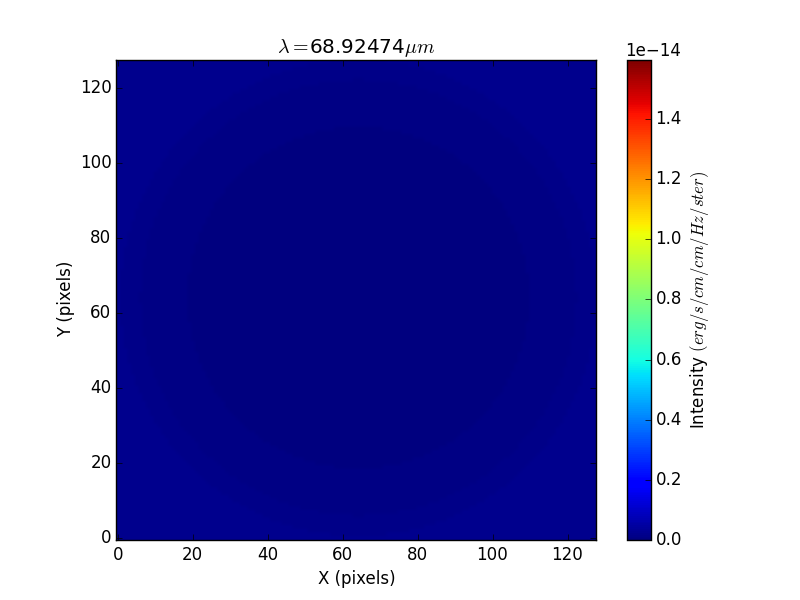
\includegraphics[width=\linewidth]{../img/output/blue.png}
\caption{The RADMC-3D output for the PACS Blue band.}\label{fig:isoblue}
\end{subfigure}
\begin{subfigure}[b]{.25\linewidth}
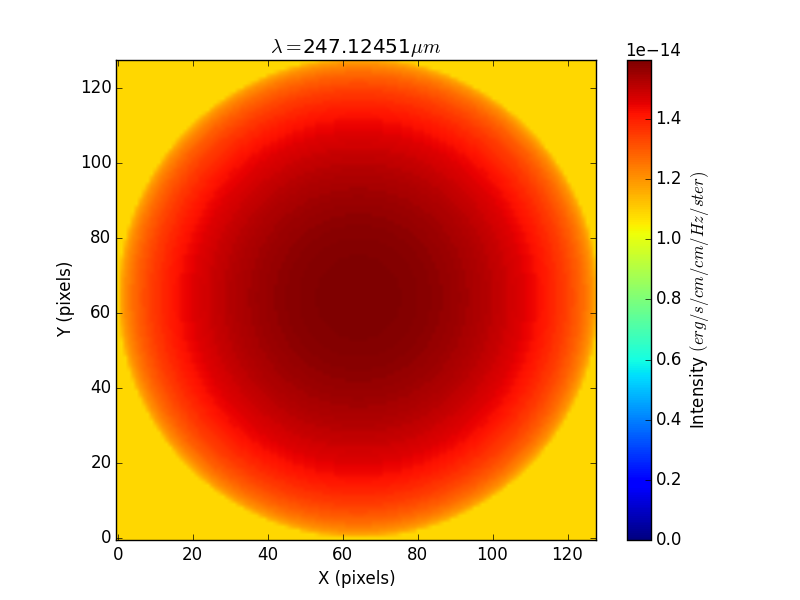
\includegraphics[width=\linewidth]{../img/output/psw.png}
\caption{The RADMC-3D output for the SPIRE PSW band.}\label{fig:isopsw}
\end{subfigure}

\begin{subfigure}[b]{.25\linewidth}
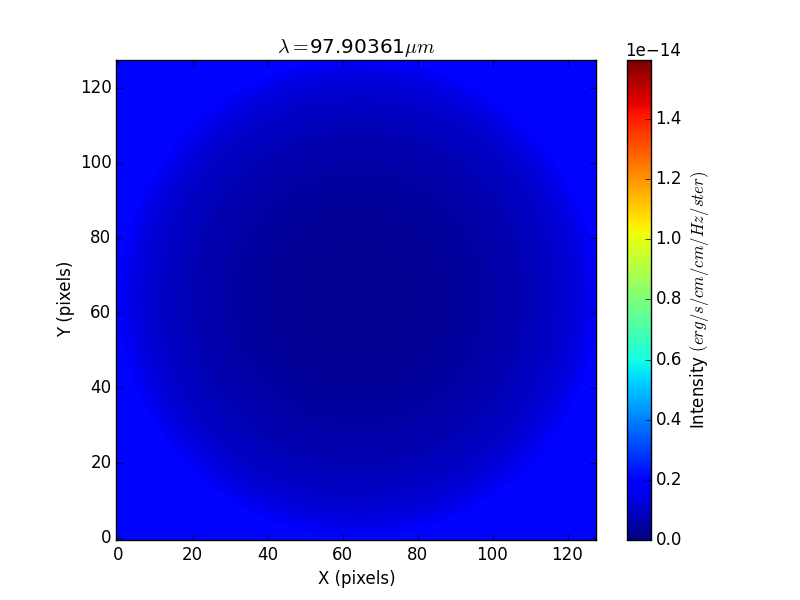
\includegraphics[width=\linewidth]{../img/output/green.png}
\caption{The RADMC-3D output for the PACS Green band.}\label{fig:isogreen}
\end{subfigure}
\begin{subfigure}[b]{.25\linewidth}
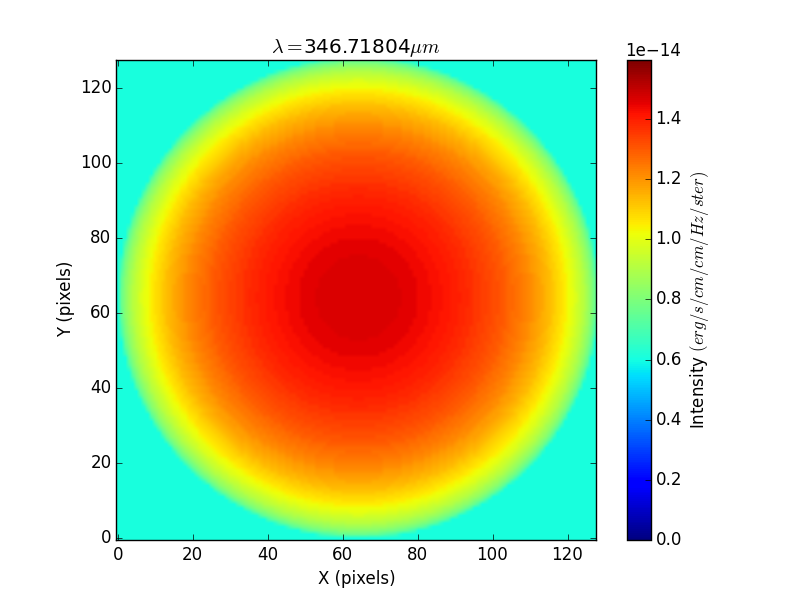
\includegraphics[width=\linewidth]{../img/output/pmw.png}
\caption{The RADMC-3D output for the SPIRE PMW band.}\label{fig:isopmw}
\end{subfigure}

\begin{subfigure}[b]{.25\linewidth}
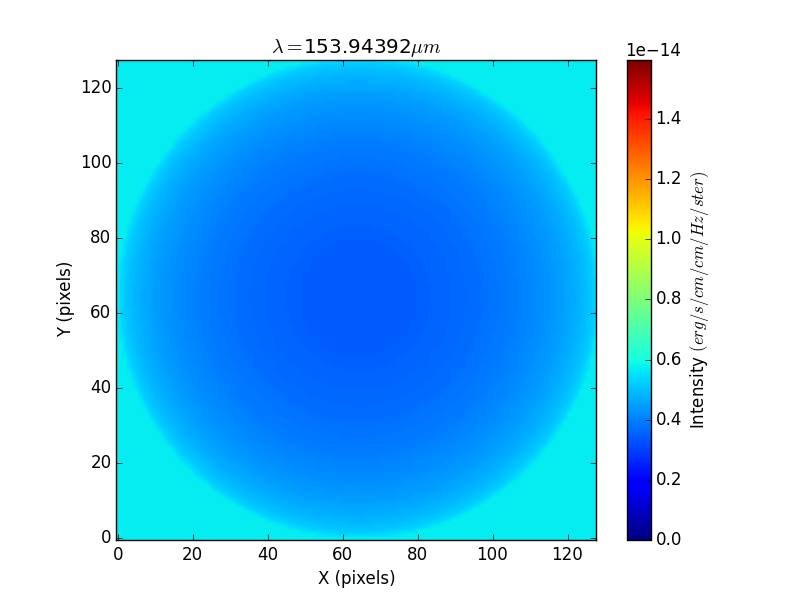
\includegraphics[width=\linewidth]{../img/output/red.png}
\caption{The RADMC-3D output for the PACS Red band.}\label{fig:isored}
\end{subfigure}
\begin{subfigure}[b]{.25\linewidth}
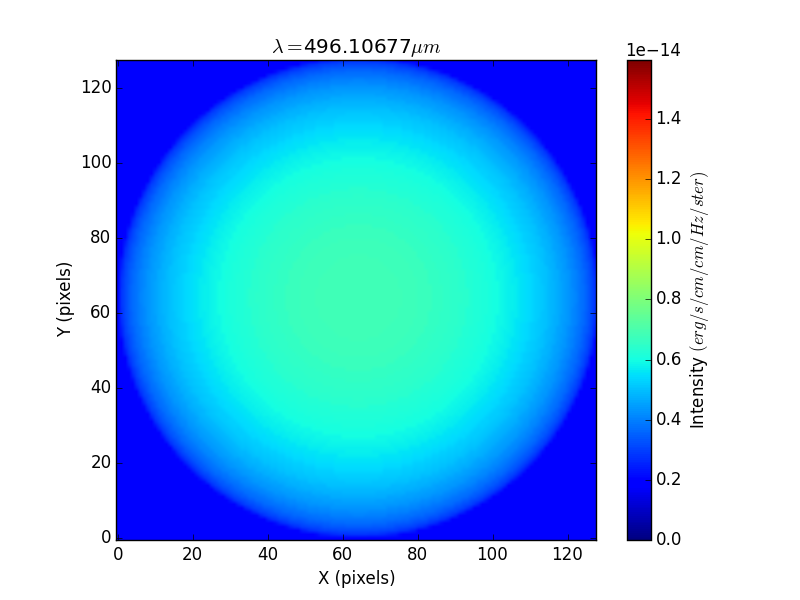
\includegraphics[width=\linewidth]{../img/output/plw.png}
\caption{The RADMC-3D output for the SPIRE PLW band.}\label{fig:isoplw}
\end{subfigure}
\caption{The RADMC-3D intensity outputs for the isothermal source at $T=10\/K$ imaged in all 6 passbands considered.} \label{fig:iso-output}
\end{figure}

Figure \ref{fig:iso-output} shows the transmission weighted intensities for an idealised isothermal source of $T=10\/K$ and $n_{dust}=10^{3}\/cm^{-3}$ in a $T=15\/K$ and $n_{dust}=1\/cm^{-3}$ background\footnote{These values of $n$ place the gas density at $10^{5}\/cm^{-3}$, above that of the coupling threshold of
$10^{4}\/cm^{-3}$ when gas begins to heat the dust. This scenario is ideal however, such that dust temperature was fixed and therefore independent of heating via gas}. The intensities vary depending on the filter used. This is to be expected, as each filter`s passband allow photons of given frequency - and therefore photons of given energy - to be detected. As the transmission curves in Figure \ref{fig:transmission} illustrates however, the intensities observed here are not the intensities that the source emits at owing the transmission coefficients. By comparing Figures \ref{fig:isoblue} through to \ref{fig:isoplw}, we observe the expected behaviour: the higher the frequency, the greater the intensity owing to the greater photon energy observed.

\begin{figure}[H]
  \captionsetup{width=0.3\textwidth}
  \centerline{\begin{minipage}[b]{0.34\linewidth}
    \centering
    \hspace{5.5ex}
    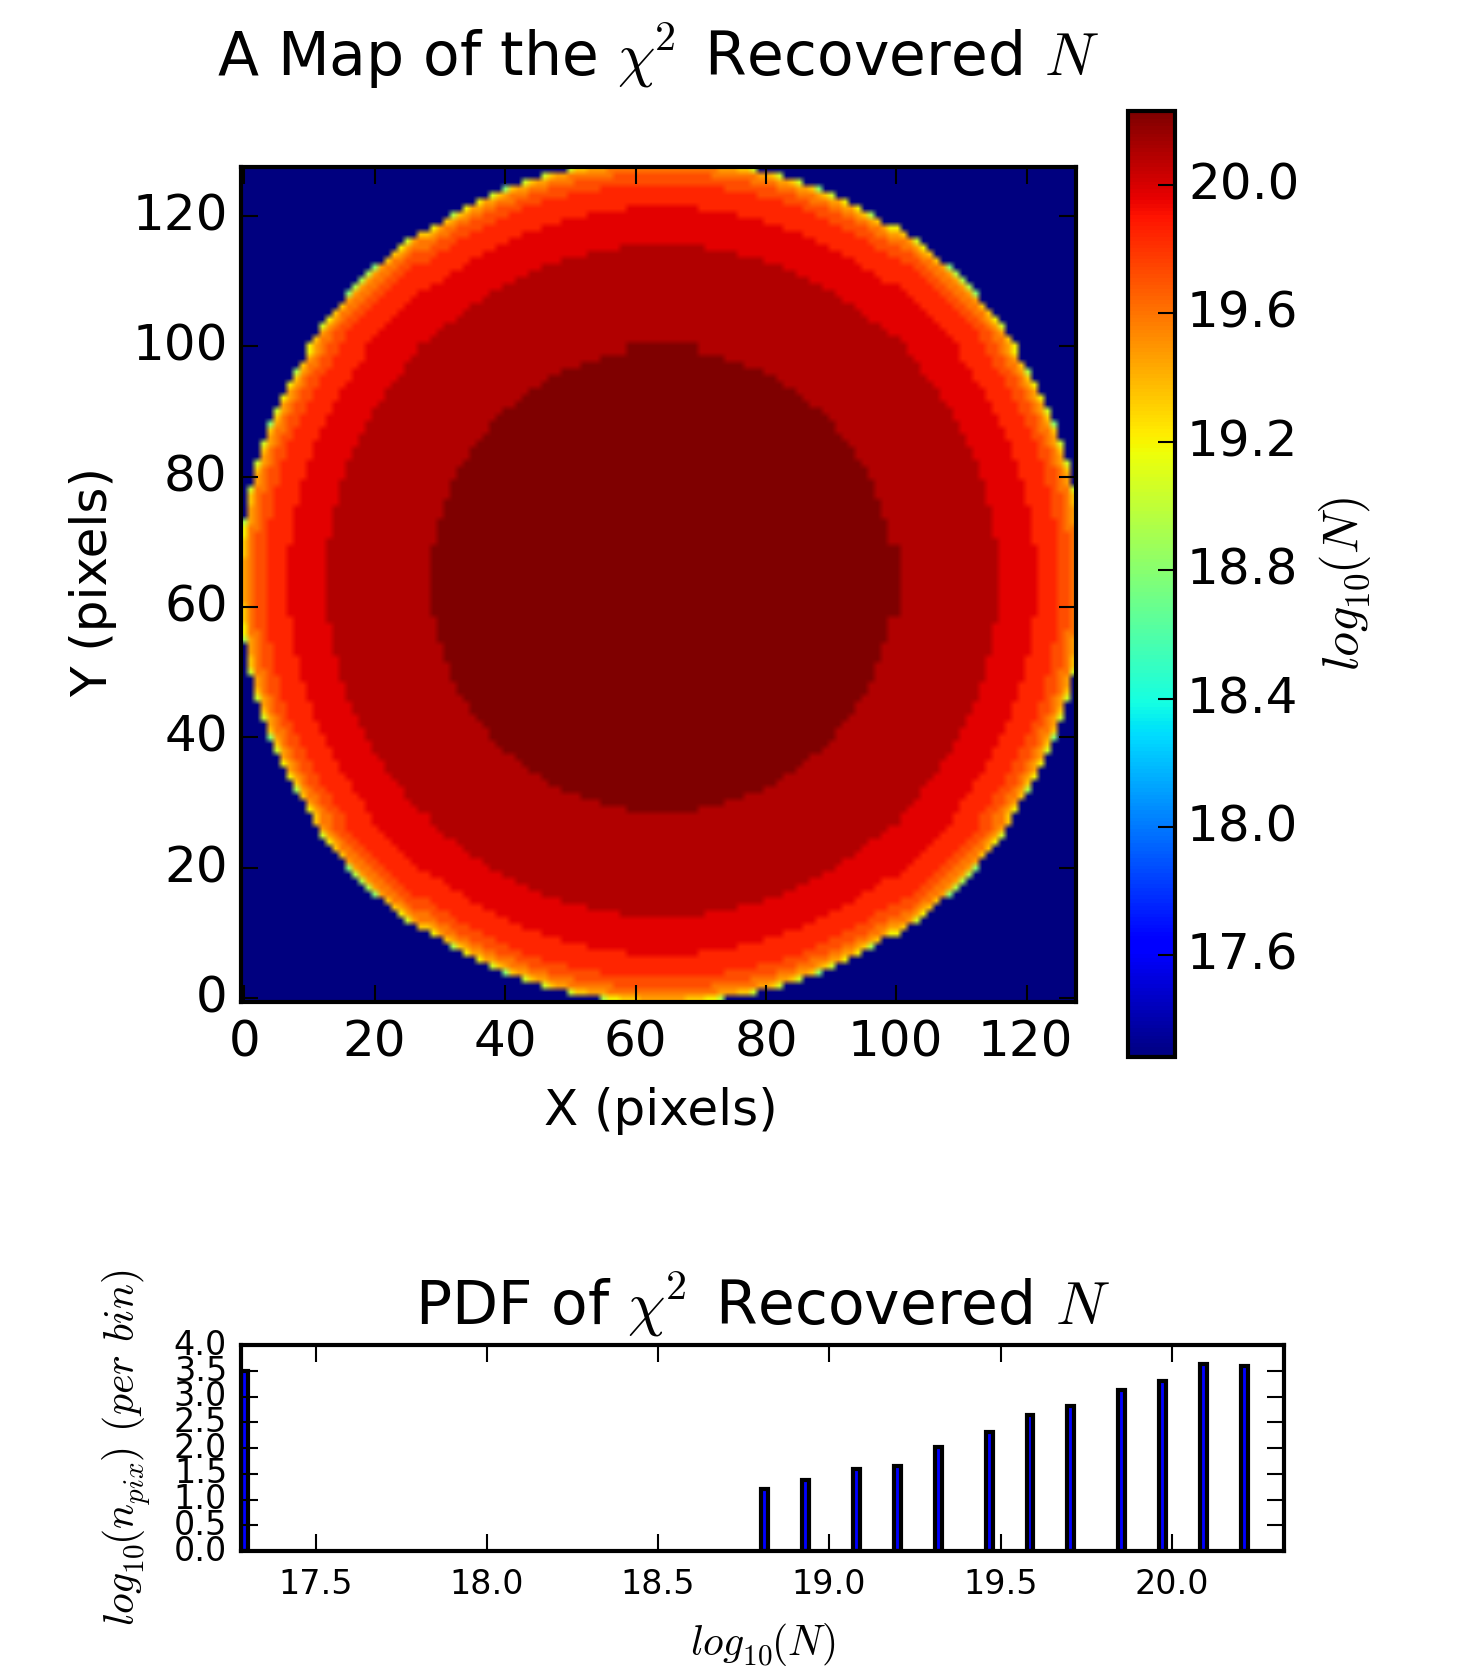
\includegraphics[width=\linewidth]{../img/sim/map_N_chi.png}
    \caption{\protect The recovered values of $N$ from the $\chi^{2}$ minimisation routine.}\label{fig:map_N_chi}
    \vspace{1.5ex}
  \end{minipage}%%
  \begin{minipage}[b]{0.34\linewidth}
    \centering
    \hspace{5.5ex}
    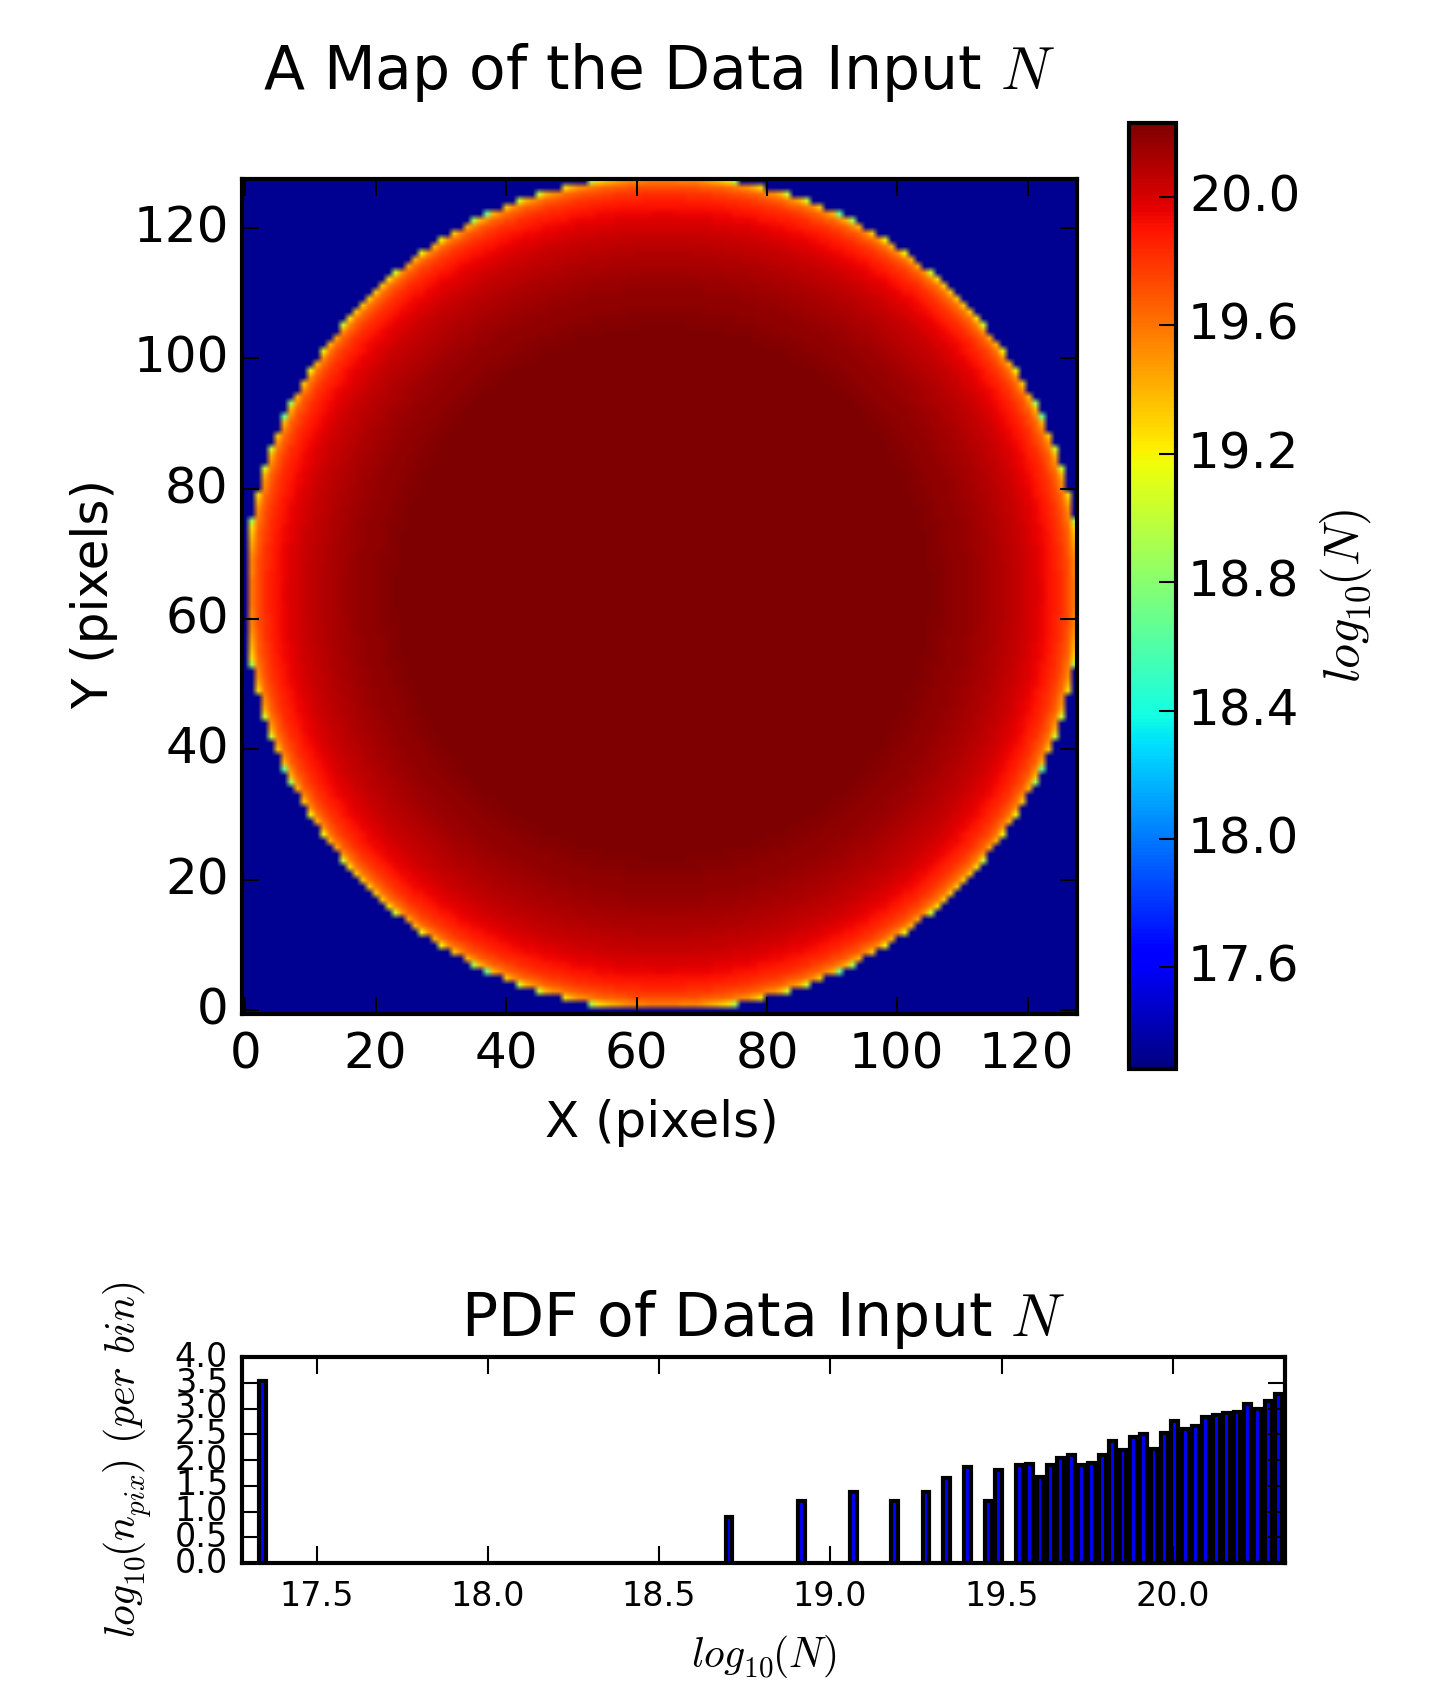
\includegraphics[width=\linewidth]{../img/sim/map_N_data.png}
    \caption{\protect The reconstructed values of $N$ from the initial input data.}\label{fig:map_N_data}
    \vspace{1.5ex}
  \end{minipage}} \\
  \centerline{\begin{minipage}[b]{0.34\linewidth}
    \centering
    \hspace{5.5ex}
    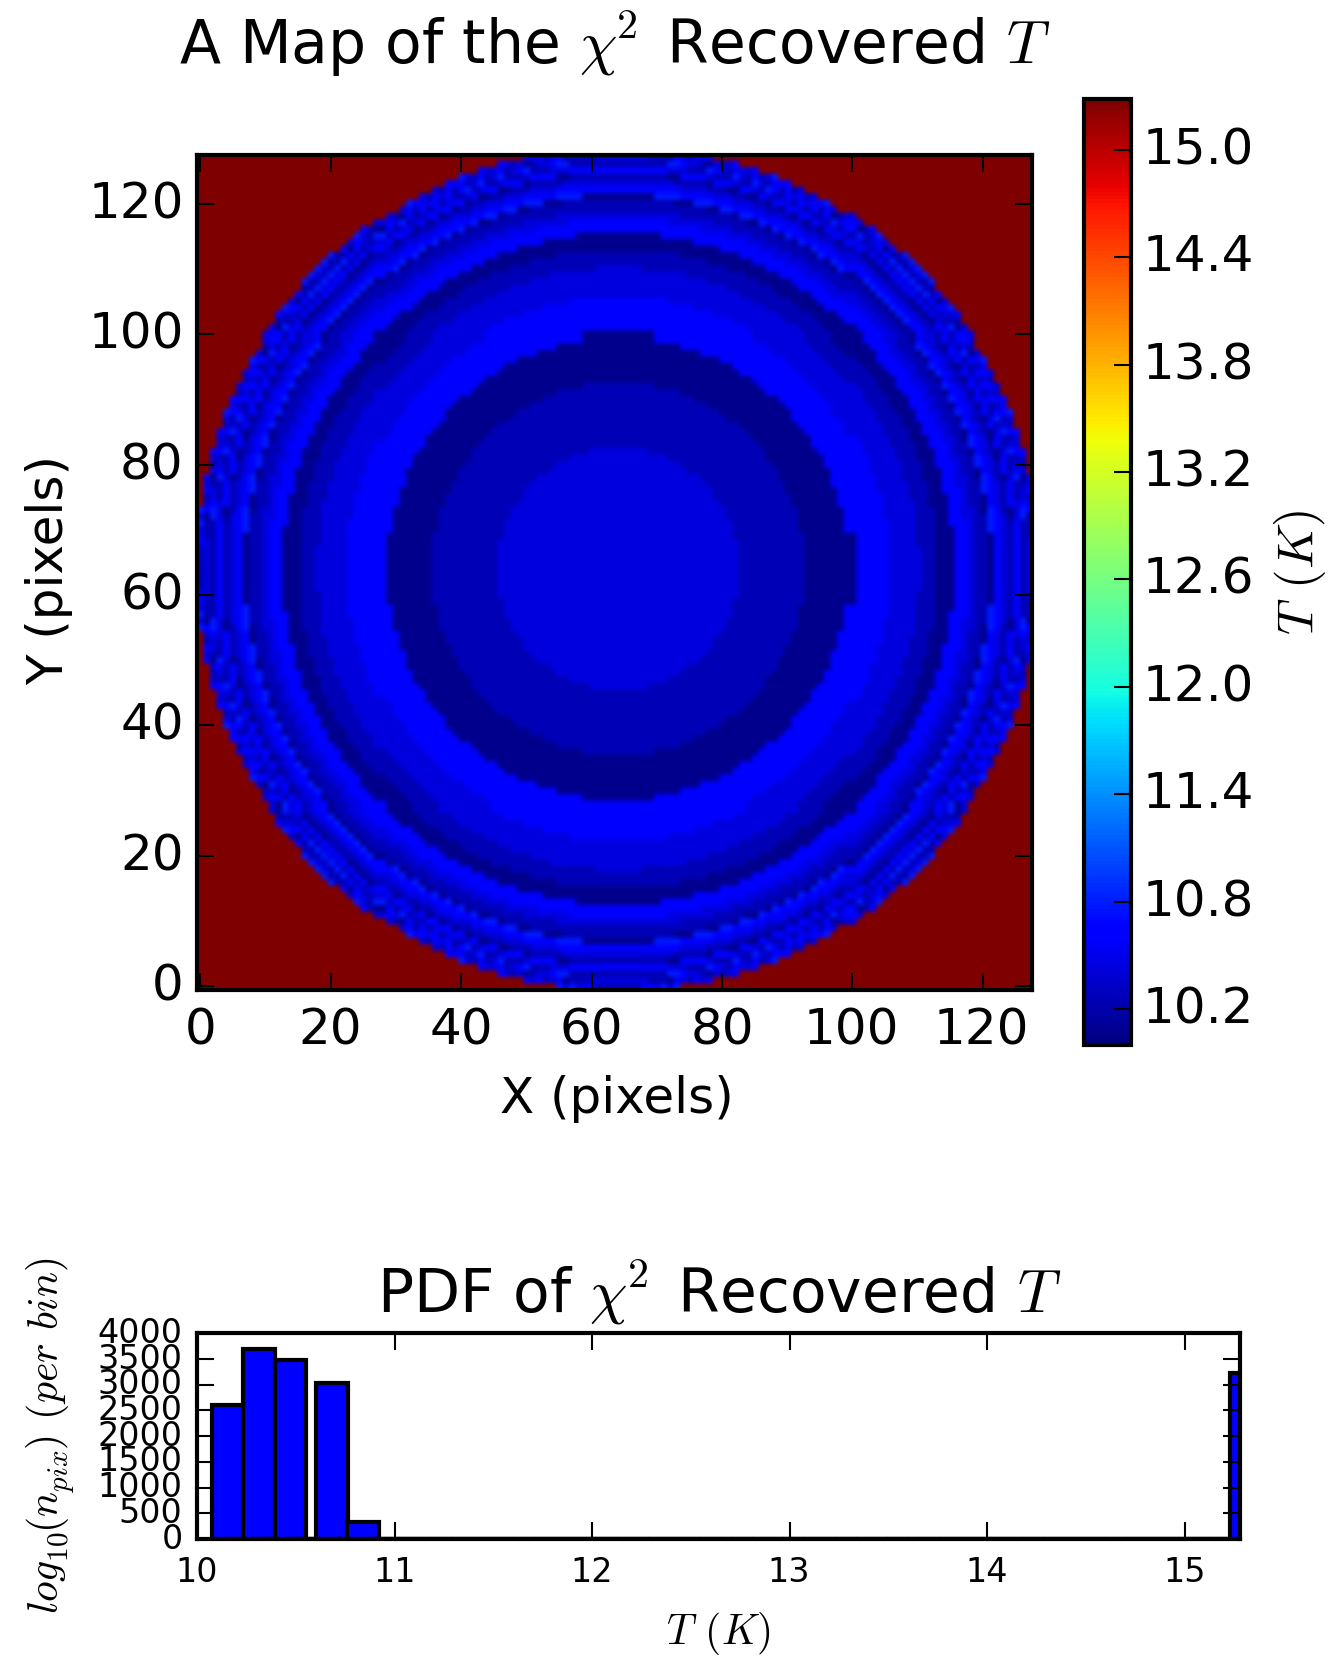
\includegraphics[width=\linewidth]{../img/sim/map_T_chi.png}
    \caption{\protect The recovered values of $T$ from the $\chi^{2}$ minimisation routine.}\label{fig:map_T_chi}
    \vspace{1.5ex}
  \end{minipage}%%
  \begin{minipage}[b]{0.34\linewidth}
    \centering
    \hspace{5.5ex}
    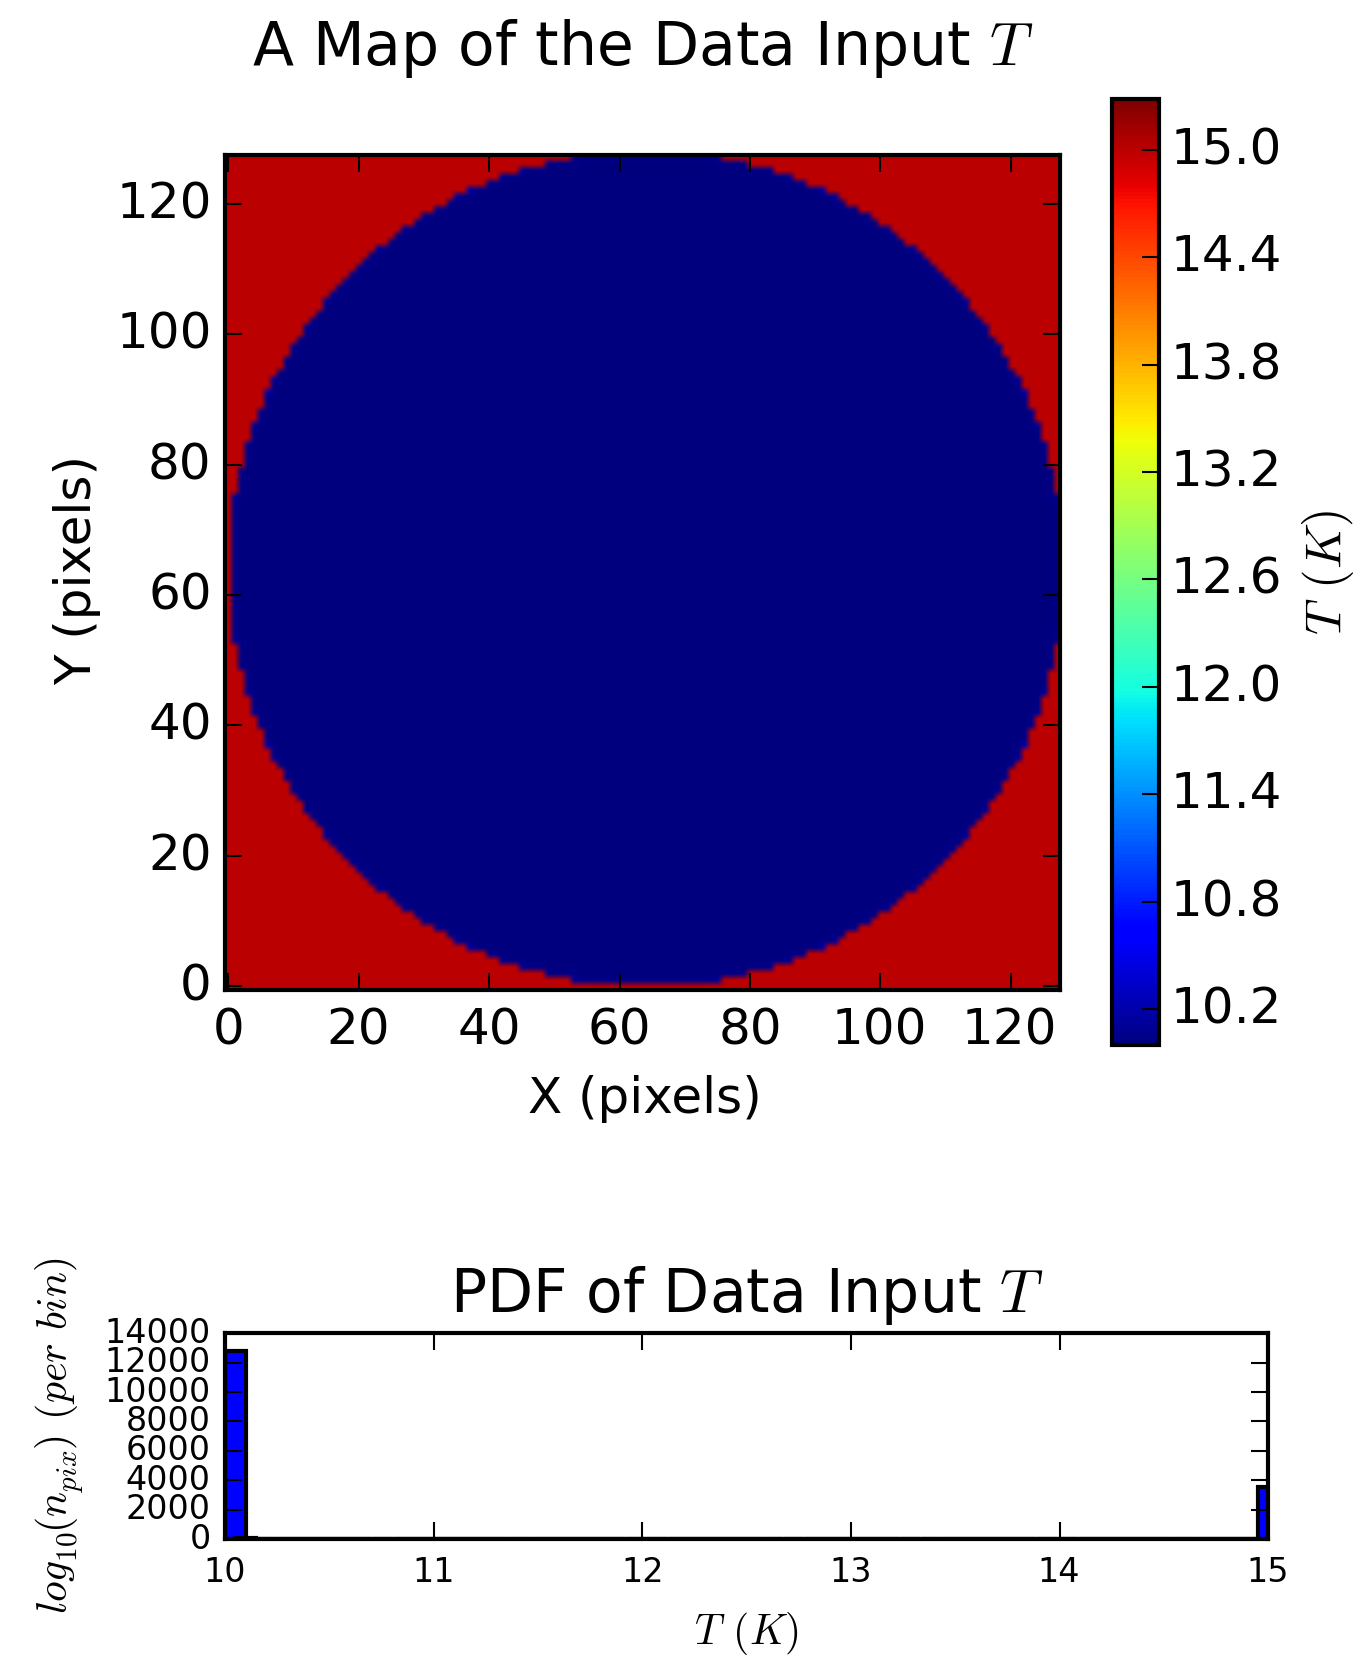
\includegraphics[width=\linewidth]{../img/sim/map_T_data.png}
    \caption{\protect The reconstructed values of $T$ from the initial input data.}\label{fig:map_T_data}
    \vspace{1.5ex}
  \end{minipage}}
\end{figure}

\begin{figure}[H]
\minipage{0.45\textwidth}
  \centering
  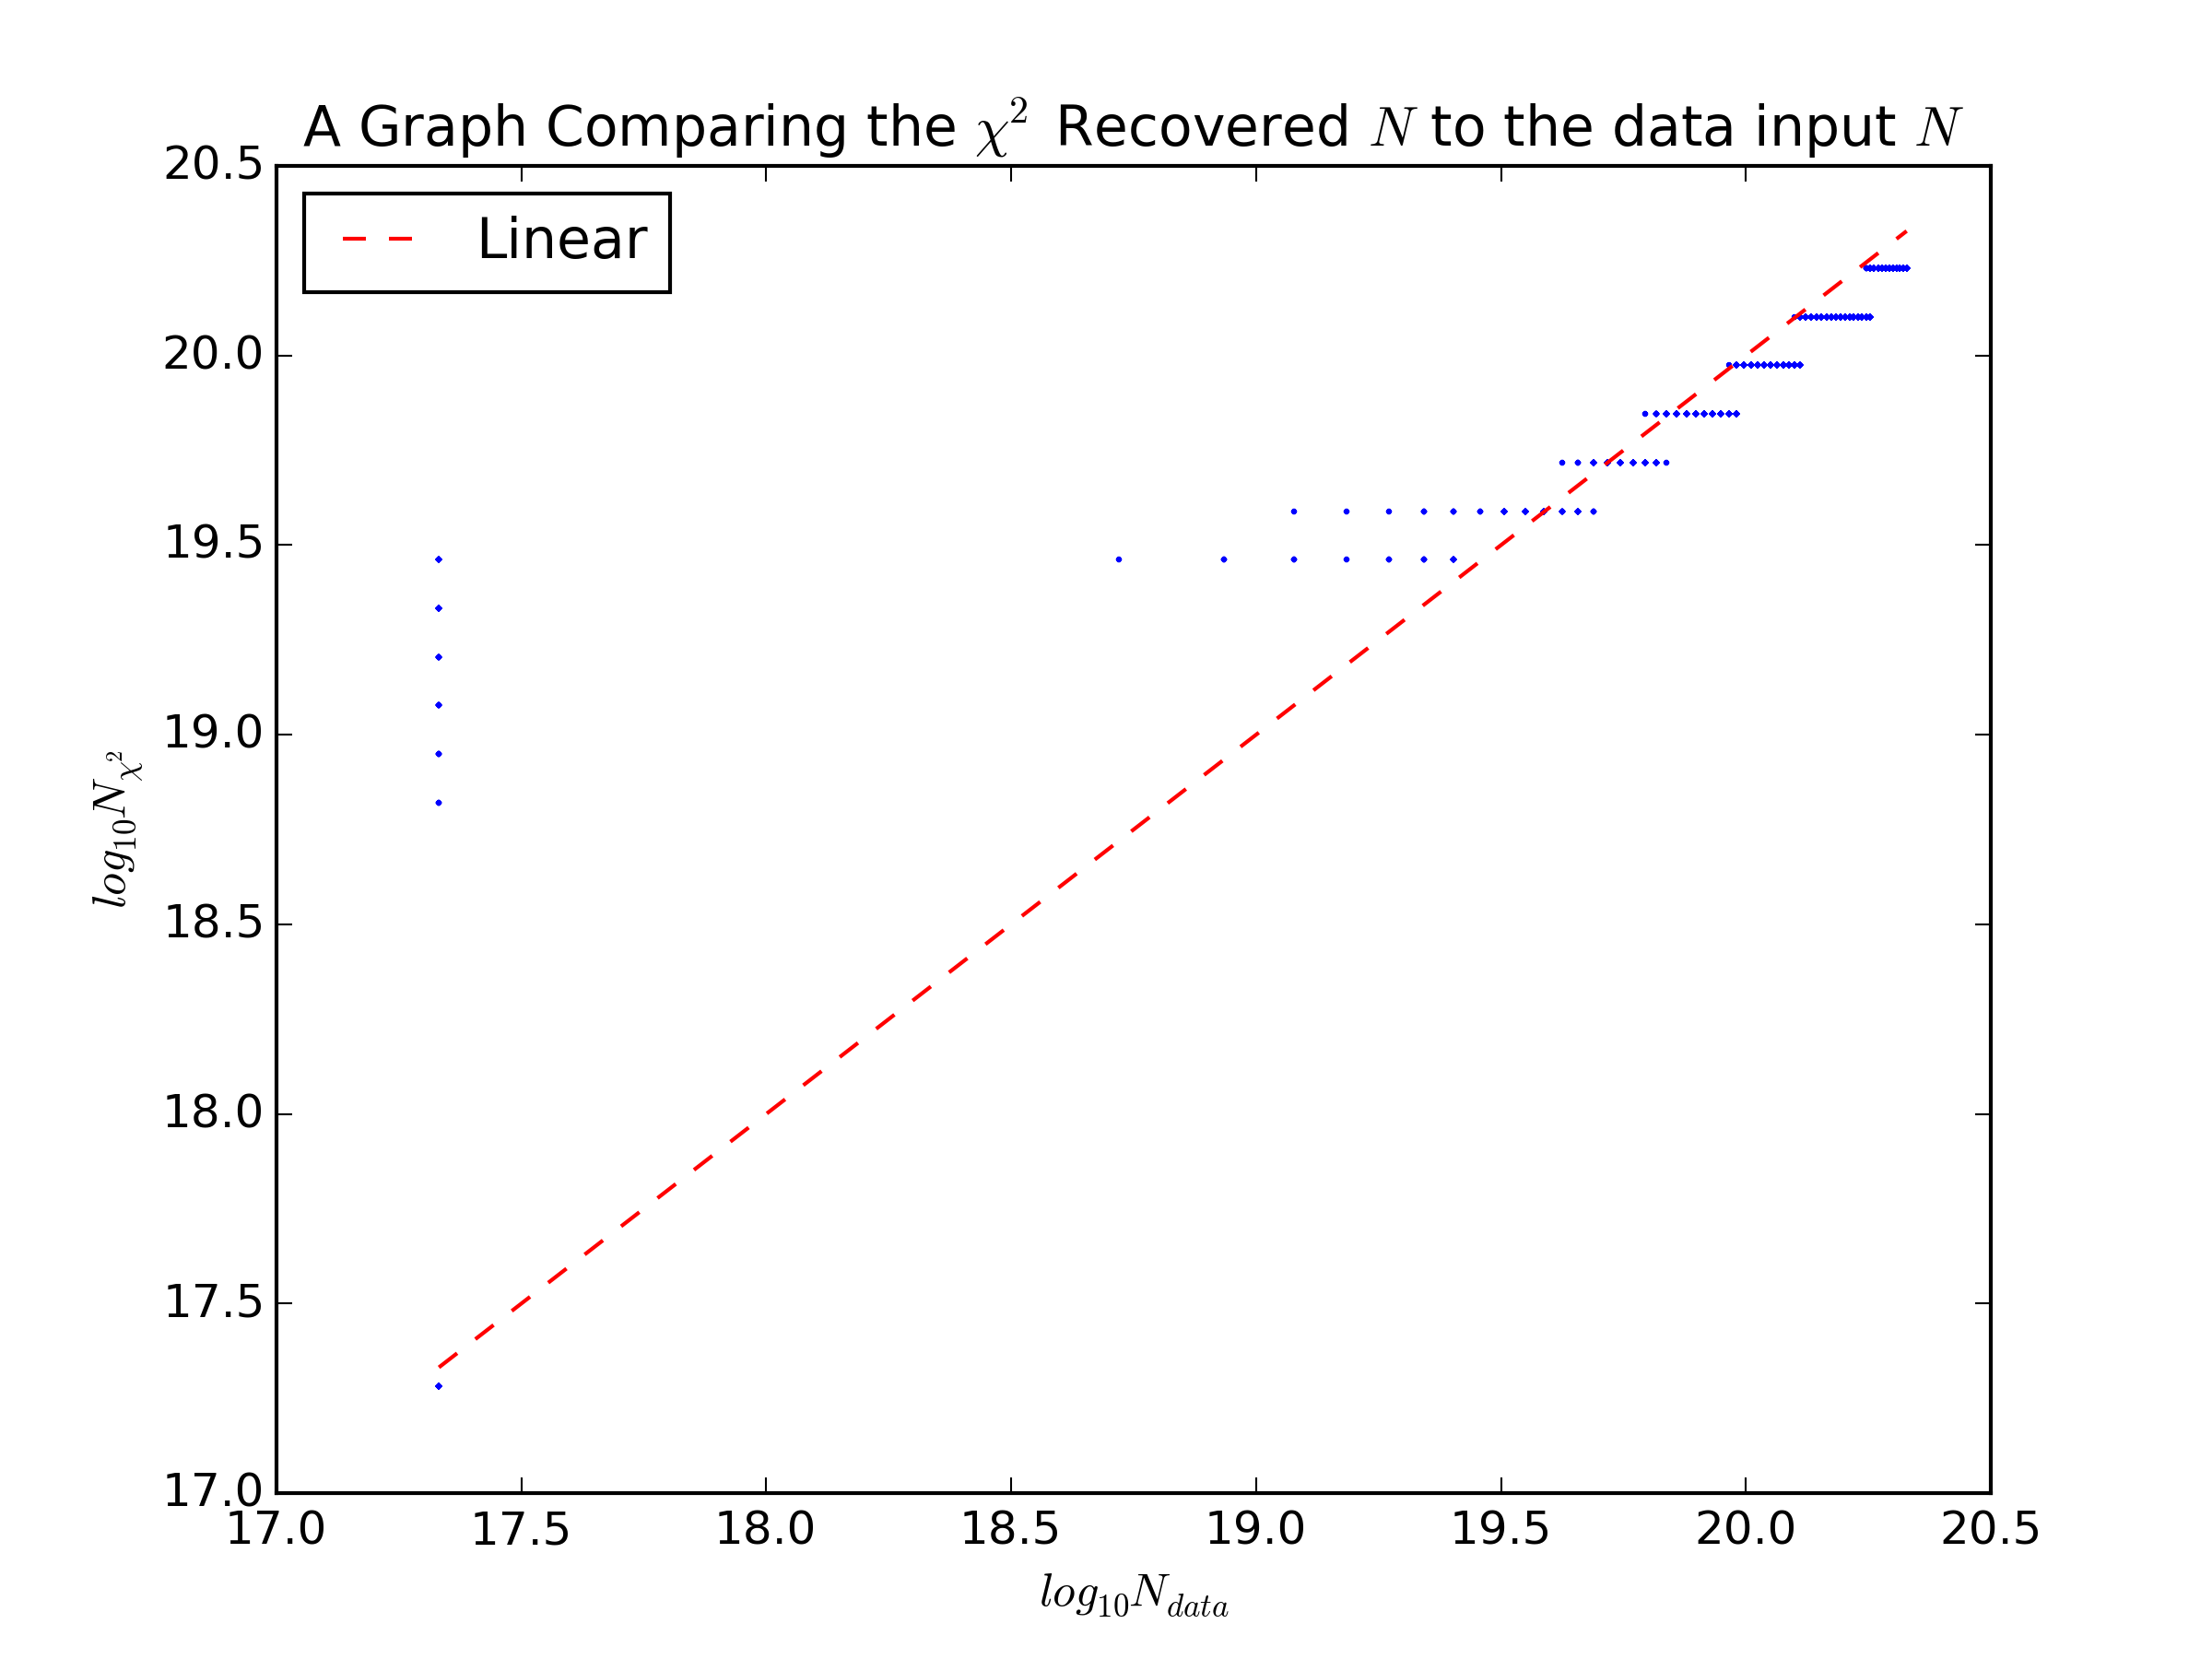
\includegraphics[width=\linewidth]{../img/sim/N.png}
  \caption{A representation of how the $\chi^{2}$ derived $N$ values compare to the initial data input $N$.}\label{fig:iso_T}
\endminipage\hfill
\minipage{0.45\textwidth}
  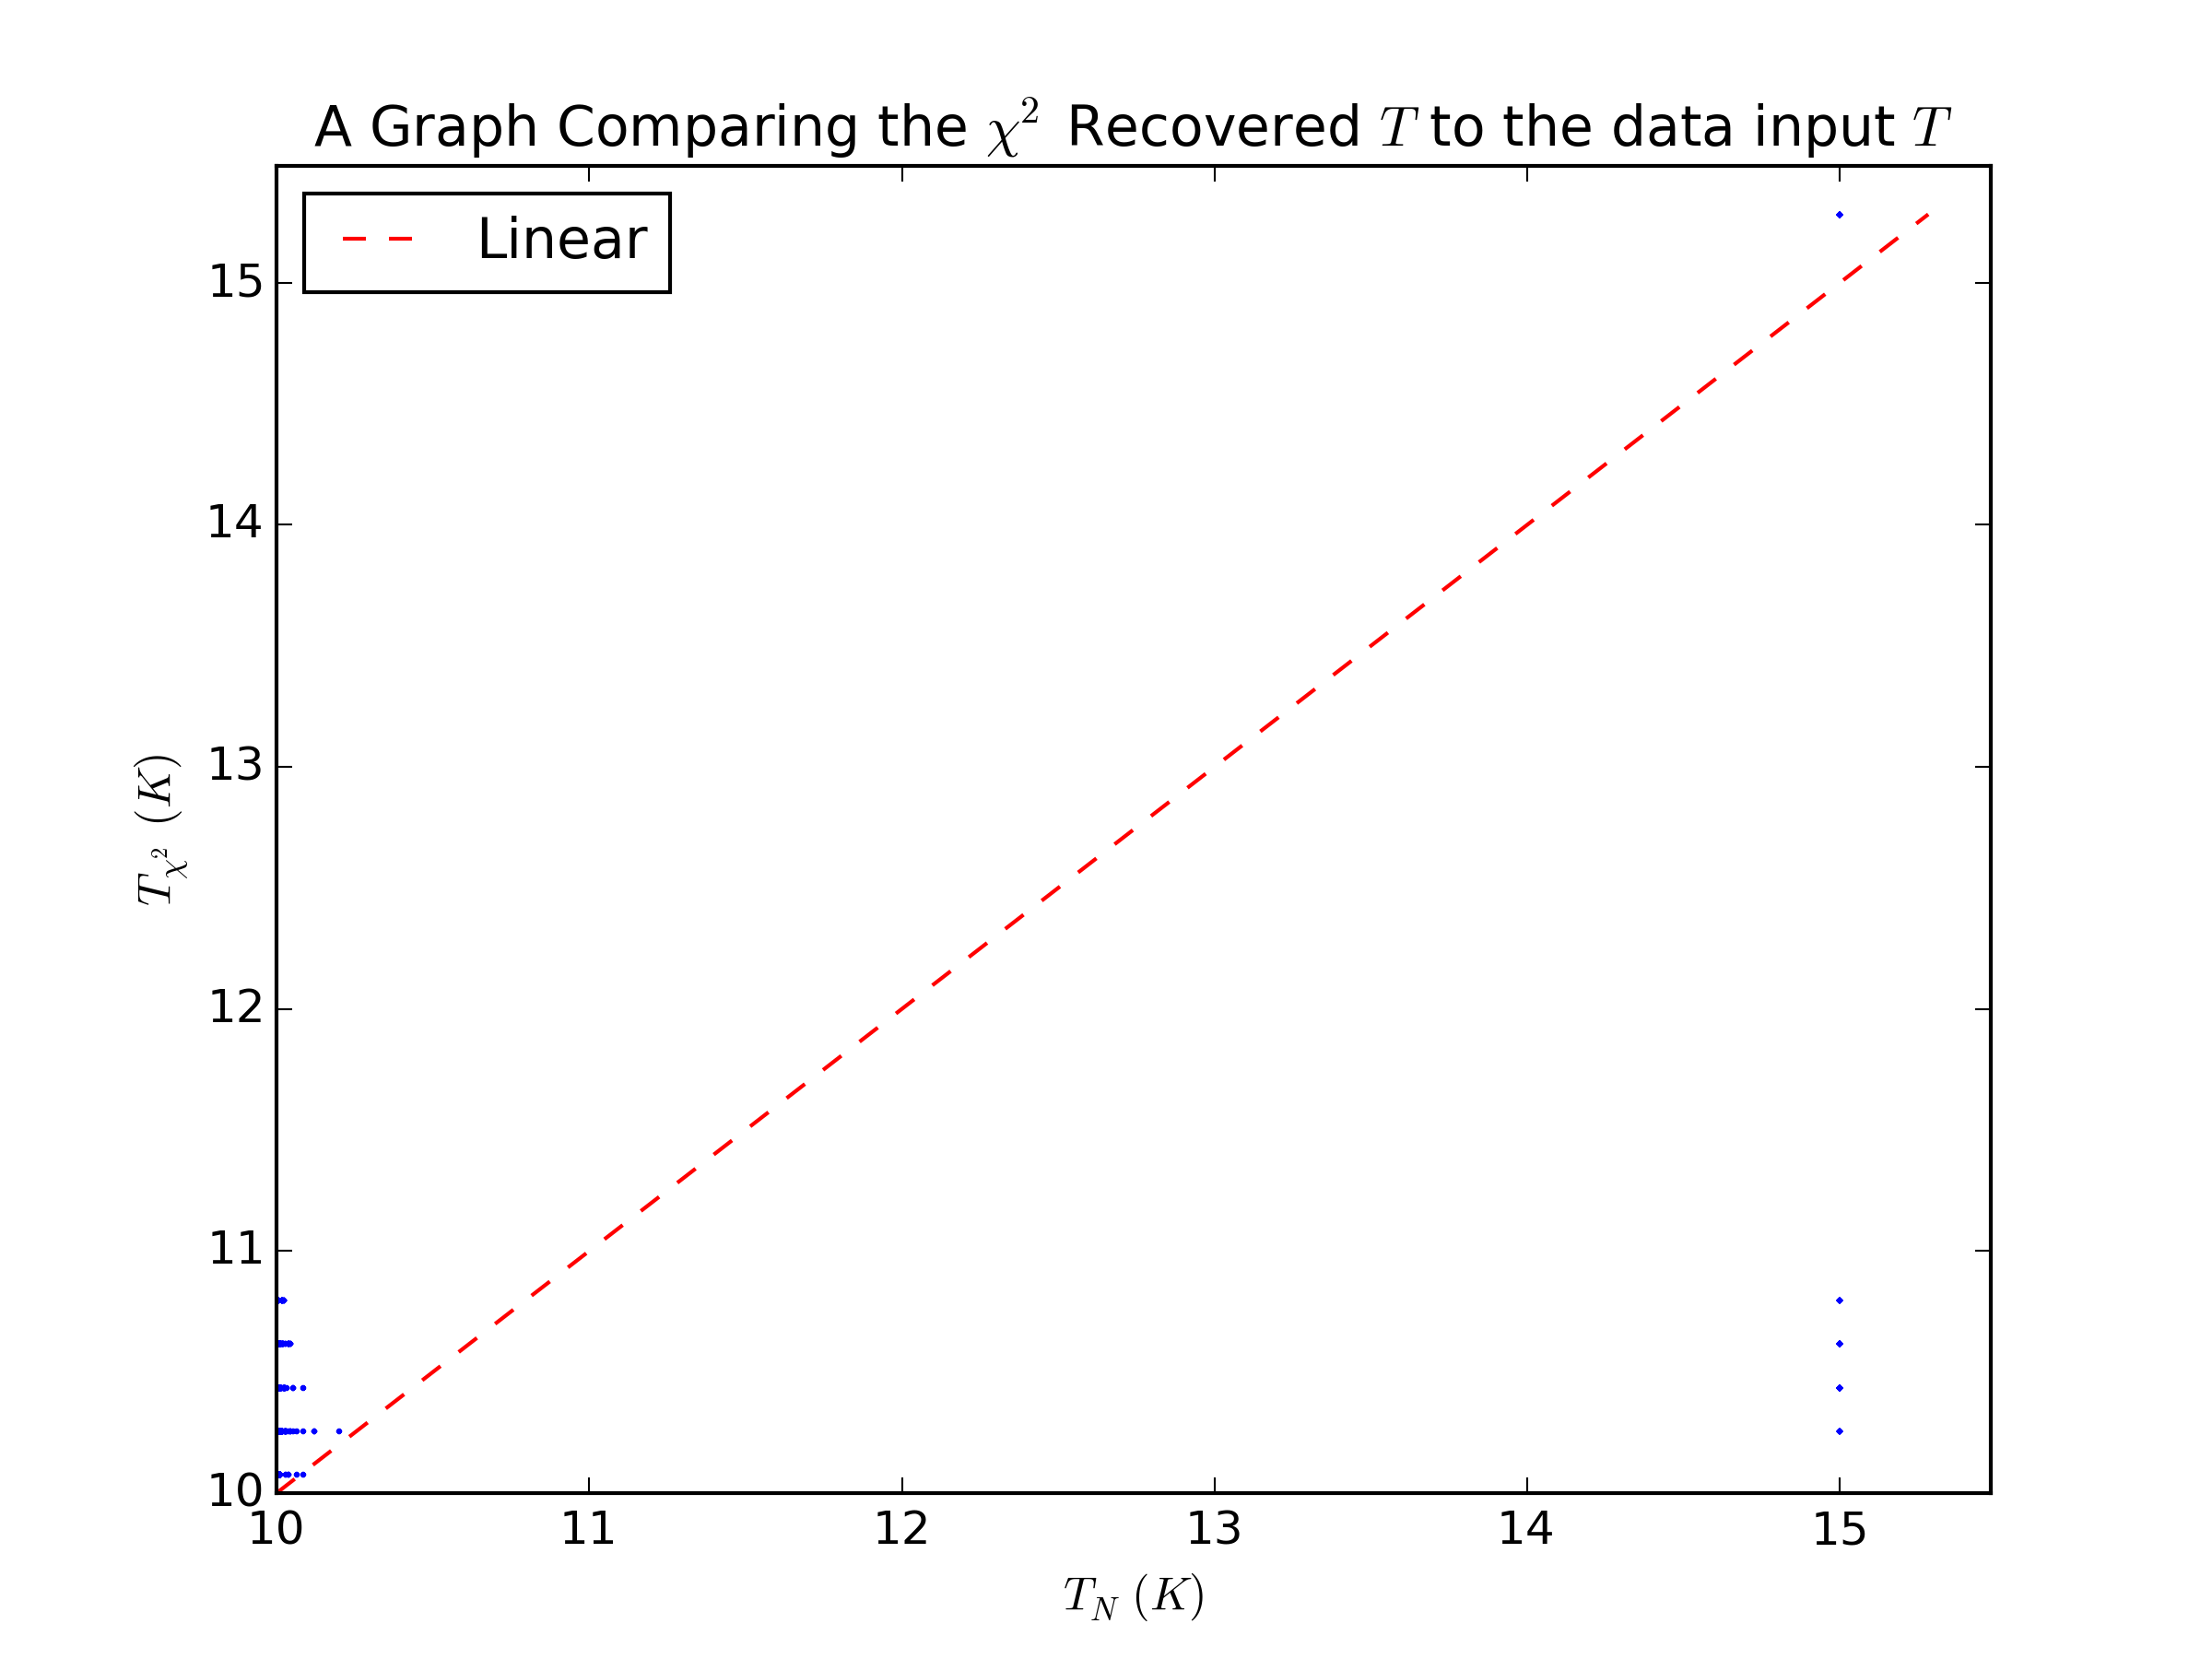
\includegraphics[width=\linewidth]{../img/sim/T.png}
  \caption{A representation of how the $\chi^{2}$ derived $T$ values compare to the initial data input $T$.}\label{fig:iso_N}
\endminipage
%\caption{A figure comparing recovered and derived values of $N$ and $T$ and how they compare. Figure \ref{fig:iso_T} shows an overestimate of the $\chi^{2}$ recovered T whilst Figure \ref{fig:iso_N} shows an underestimate the $\chi^{2}$ recovered $N$.}
\end{figure}

\begin{figure}[H]
  \centering
  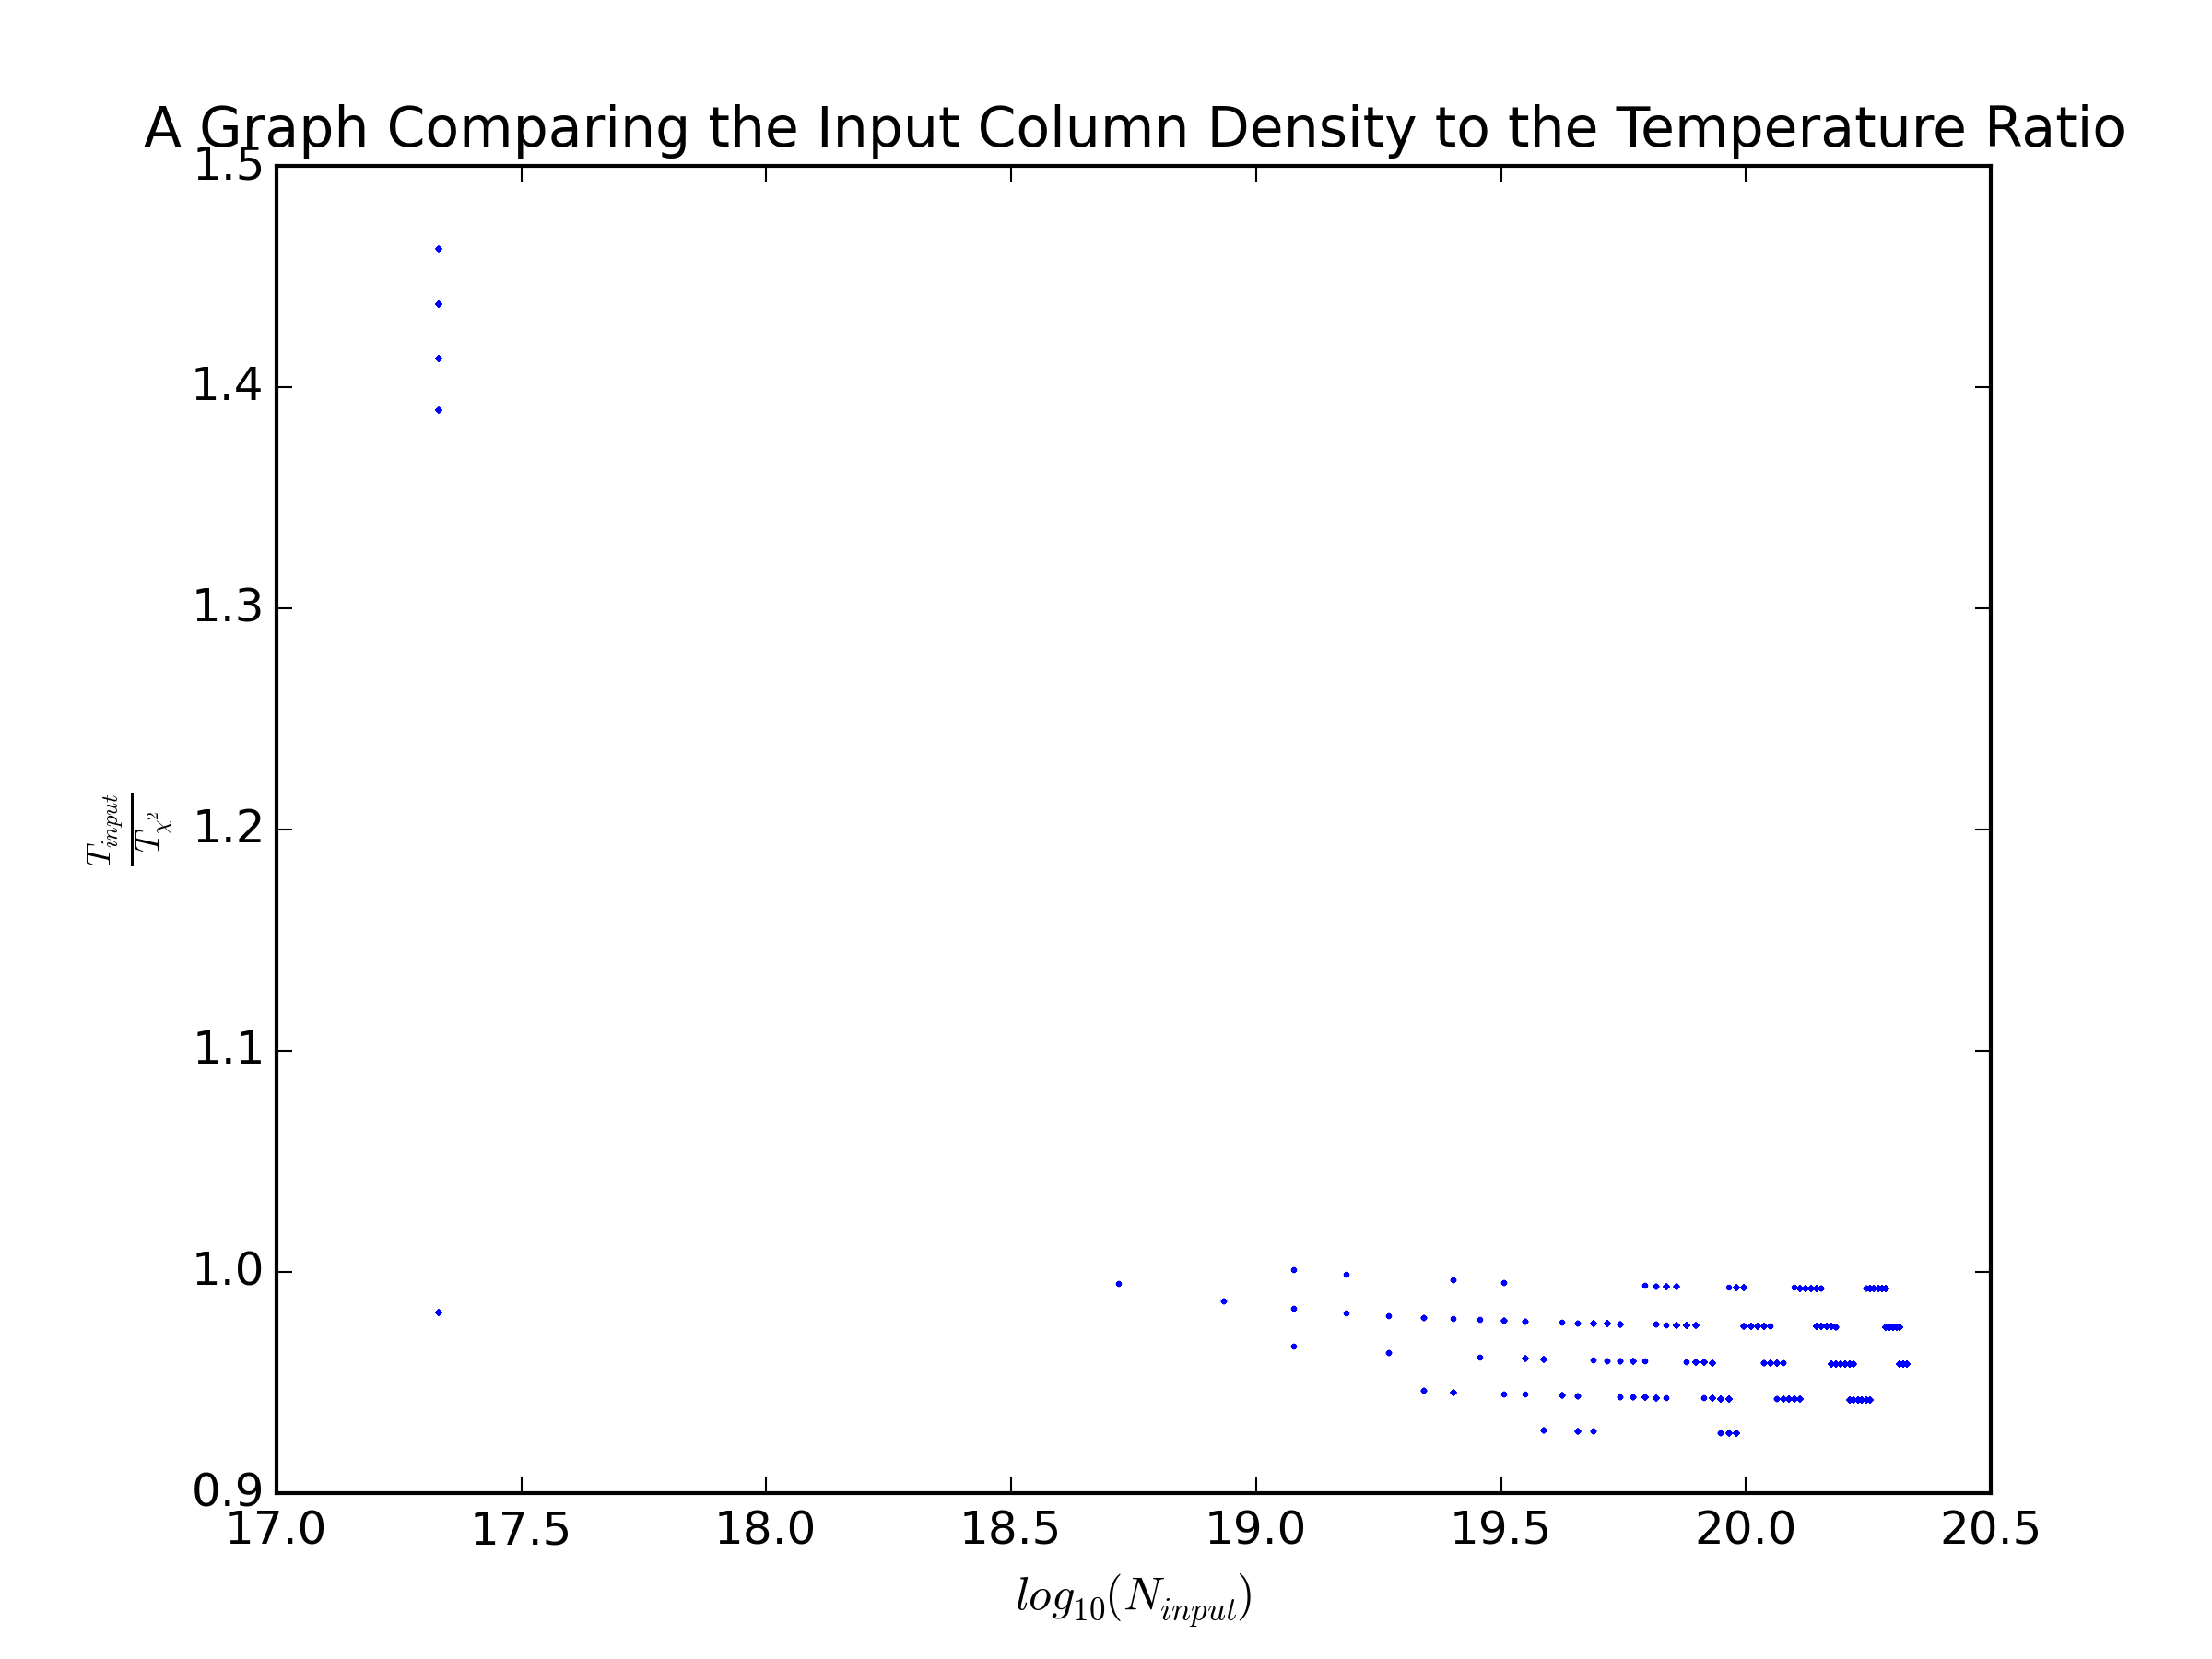
\includegraphics[width=0.45\linewidth]{../img/sim/T_ratio_inp.png}
  \caption{A plot showing how the ratio of $T_{input}/T_{\chi^{2}}$ varies with the input $T$.}\label{fig:T_ratio}
%\caption{A figure comparing recovered and derived values of $N$ and $T$ and how they compare. Figure \ref{fig:iso_T} shows an overestimate of the $\chi^{2}$ recovered T whilst Figure \ref{fig:iso_N} shows an underestimate the $\chi^{2}$ recovered $N$.}
\end{figure}

Figure \ref{fig:iso-output} is an isothermal sphere, meaning that very few line of sight temperature variations are present. As such, a single $T$ assumption along the line of sight is accurate, implying that the modified blackbody in Equation \ref{eq:mbb-int} is a good fit to the data. The $\chi^{2}$ recovered values of $N$ and $T$ (by fitting Equation \ref{eq:mbb-int}), along with the data derived values, are shown in Figures \ref{fig:map_N_chi}, \ref{fig:map_N_data},
\ref{fig:map_T_chi} and \ref{fig:map_T_data}. The $\chi^{2}$ recovered values were derived from fitting to the SPIRE bands \textit{only}, as the PACS bands were found to be inaccurate descriptors of dust emission intensity at the temperatures considered. Figures \ref{fig:map_N_chi}, \ref{fig:map_N_data},
\ref{fig:map_T_chi} and \ref{fig:map_T_data} also show PDFs of the data where $n_{pix}$ is the number of pixels per bin.

By direct comparison of Figure \ref{fig:map_N_chi} with Figure \ref{fig:map_N_data} it is observed that the $\chi^{2}$ recovered $N$ values match the derived $N$ values well at large $N$ (though the $\chi^{2}$ values are understimated at low $N$). This is also shown in Figure \ref{fig:iso_N}, which compares the $\chi^{2}$ $N$ to the data input
$N$. Within Figure \ref{fig:iso_N}, the red line represents the linear relationship expected were the $\chi^{2}$ recovered values to match the data derived value exactly. It clearly shows a wide degree of scatter across both input
$N$ and $\chi^{2}$ $N$. Figure \ref{fig:iso_N} shows that $\chi^{2}$ minimisation produces one estimate of $N$ for a large degree of input $N$, especially at lower values of $N$. Of note here is the fact that this is especially true of high $N$, where the values differ by a smaller degree relative to the low $N$ regime where the spread is greater. This is also illustrated in the ratios shown in Figures \ref{fig:T_ratio}.

Comparing Figure \ref{fig:map_T_chi} with Figure \ref{fig:map_T_data} we see that $\chi^{2}$ largely overestimates $T$ relative to the data derived $T$. It also finds that the temperature decreases radially from the centre of the sphere, whereas Figure \ref{fig:map_T_data} shows $T$ to be constant. This is also evident in the PDFs in both figures: Figure \ref{fig:map_T_data} shows 2 discrete bins at $10\/K$ and
$15\/K$, whereas Figure \ref{fig:map_T_chi} displays a peak above $10\/K$ that decreases at $11\/K$, as well as another peak above $15\/K$. The overestimate of $T$ is evident here, though the shape of PDFs in Figures \ref{fig:map_N_chi} and \ref{fig:map_N_data} show similar shapes even with the underestimate evident. Likewise, the PDFs in Figures
\ref{fig:map_T_chi} and \ref{fig:map_T_data} exhibit the same behaviour. Whilst the shape of the PDF themselves remain similar, the $\chi^{2}$ recovered quantities suffer from the discretisation of the values used to generate them, as evidenced by the discrete peaks in the PDFs. This is not evident in the data derived quantities, which show a smoother PDF. Furthermore, the spheres themselves are generated with discrete pixels, resulting in the column density (and temperature along the line of sight as this quantity is column weighted) increasing in steps rather than transitioning smoothly. This effect is exaggerated in the $\chi^{2}$ recovery, as both $N$ and $T$ show banding.


\pagebreak
\section{Arepo data} \label{sec:sph}


\begin{figure}[H]
\centering

\begin{subfigure}[b]{.35\linewidth}
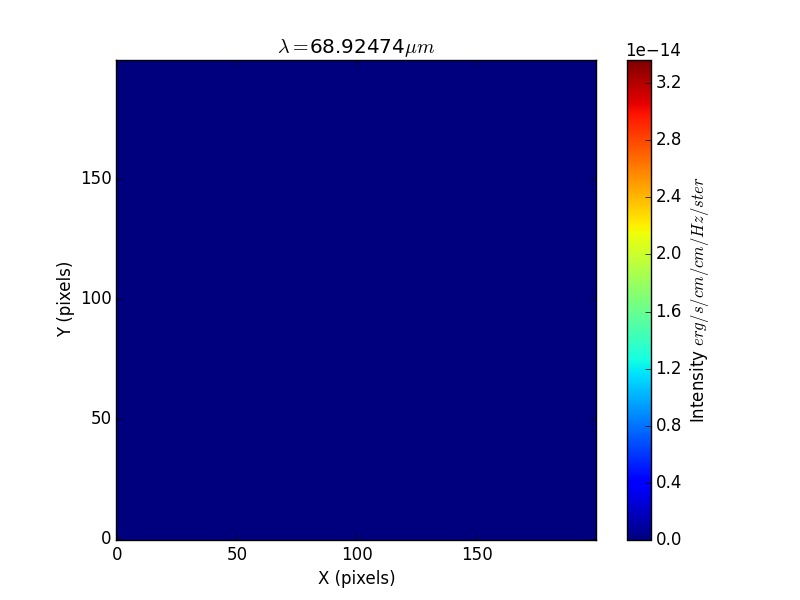
\includegraphics[width=\linewidth]{../img/sph/blue.png}
\caption{The RADMC-3D output for the PACS Blue band.}\label{fig:sphblue}
\end{subfigure}
\begin{subfigure}[b]{.35\linewidth}
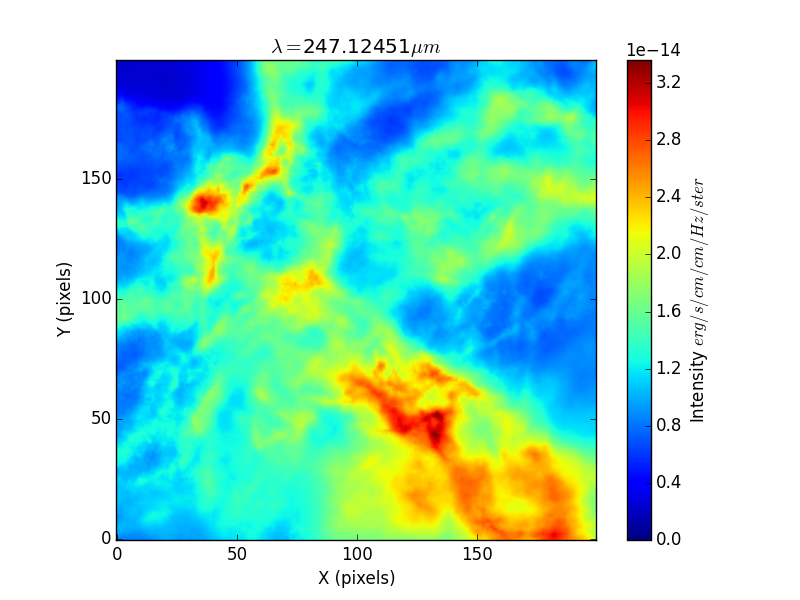
\includegraphics[width=\linewidth]{../img/sph/psw.png}
\caption{The RADMC-3D output for the SPIRE PSW band.}\label{fig:sphpsw}
\end{subfigure}

\begin{subfigure}[b]{.35\linewidth}
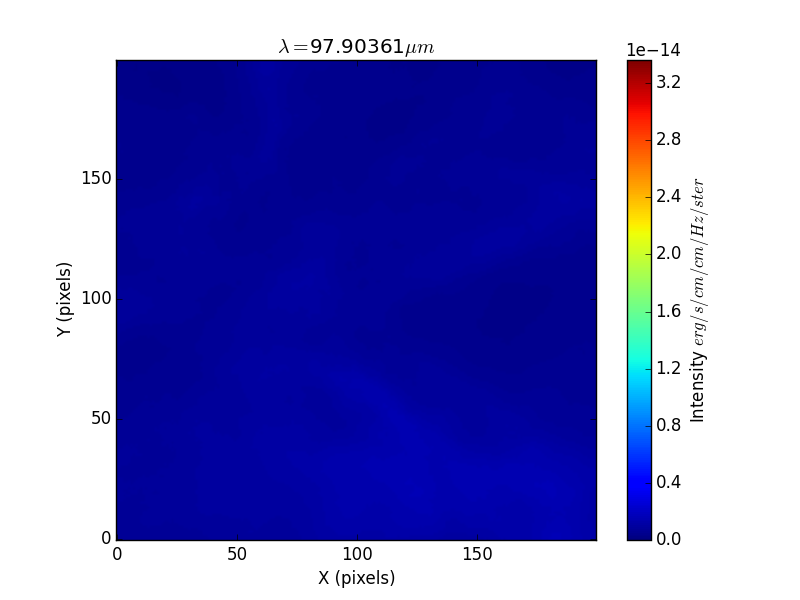
\includegraphics[width=\linewidth]{../img/sph/green.png}
\caption{The RADMC-3D output for the PACS Green band.}\label{fig:sphgreen}
\end{subfigure}
\begin{subfigure}[b]{.35\linewidth}
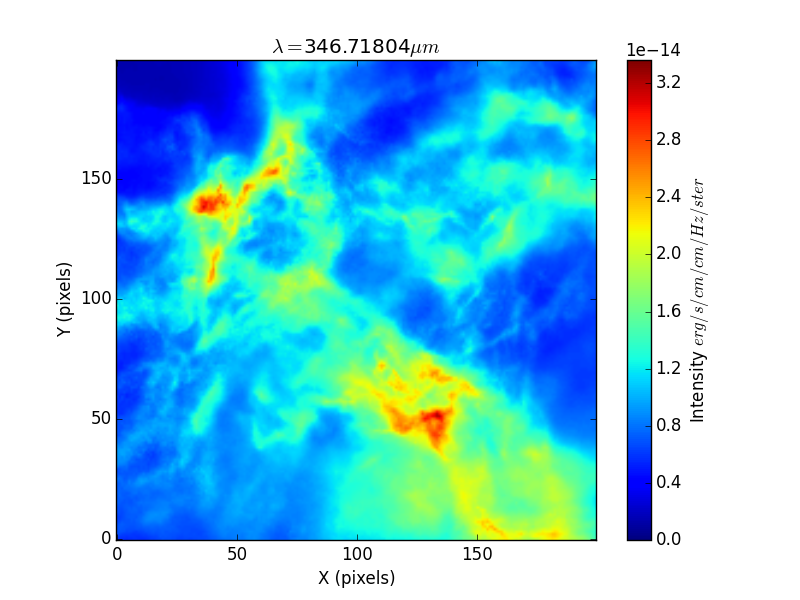
\includegraphics[width=\linewidth]{../img/sph/pmw.png}
\caption{The RADMC-3D output for the SPIRE PMW band.}\label{fig:sphpmw}
\end{subfigure}

\begin{subfigure}[b]{.35\linewidth}
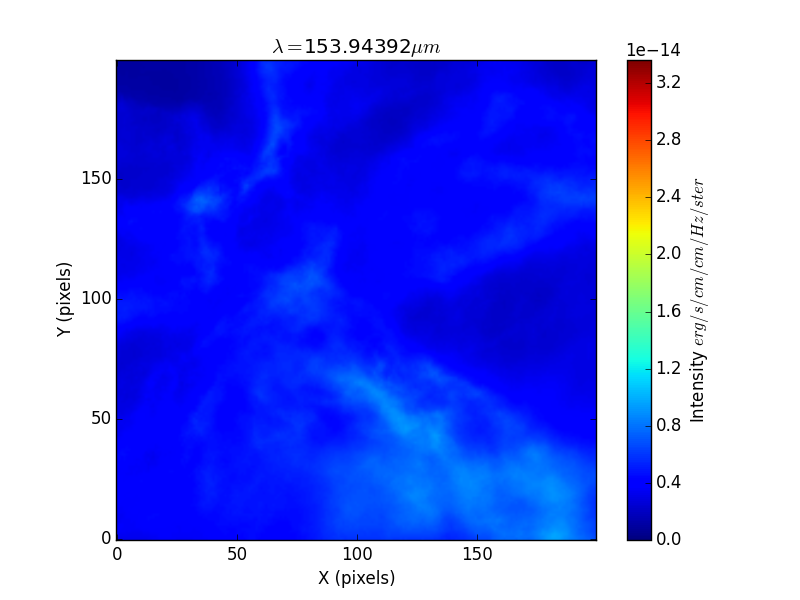
\includegraphics[width=\linewidth]{../img/sph/red.png}
\caption{The RADMC-3D output for the PACS Red band.}\label{fig:sphred}
\end{subfigure}
\begin{subfigure}[b]{.35\linewidth}
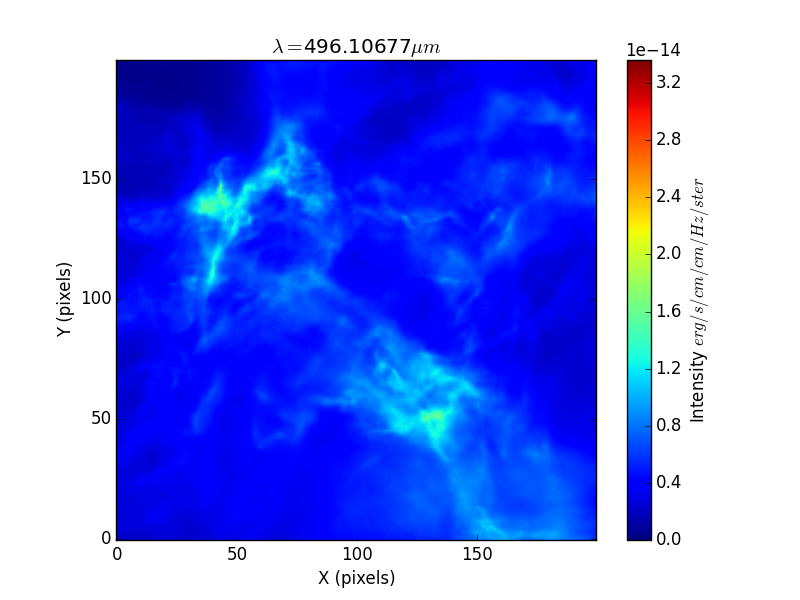
\includegraphics[width=\linewidth]{../img/sph/plw.png}
\caption{The RADMC-3D output for the SPIRE PLW band.}\label{fig:sphplw}
\end{subfigure}
\caption{The RADMC-3D intensity outputs for the Arepo data imaged in all 6 passbands considered.} \label{fig:sph-output}
\end{figure}

Figure \ref{fig:sph-output} shows the RADMC-3D image outputs for the Arepo data. The same behaviour is observed here, as was observed in Figure \ref{fig:iso-output}. Figures \ref{fig:map_N_chi_sph}, \ref{fig:map_N_data_sph},
\ref{fig:map_T_chi_sph} and \ref{fig:map_T_data_sph} illustrate the $\chi^{2}$ recovered values of $N$ and $T$, as well as the data input derived equivalents.

\begin{figure}[H]
  \captionsetup{width=0.32\textwidth}
  \centerline{\begin{minipage}[b]{0.34\linewidth}
    \centering
    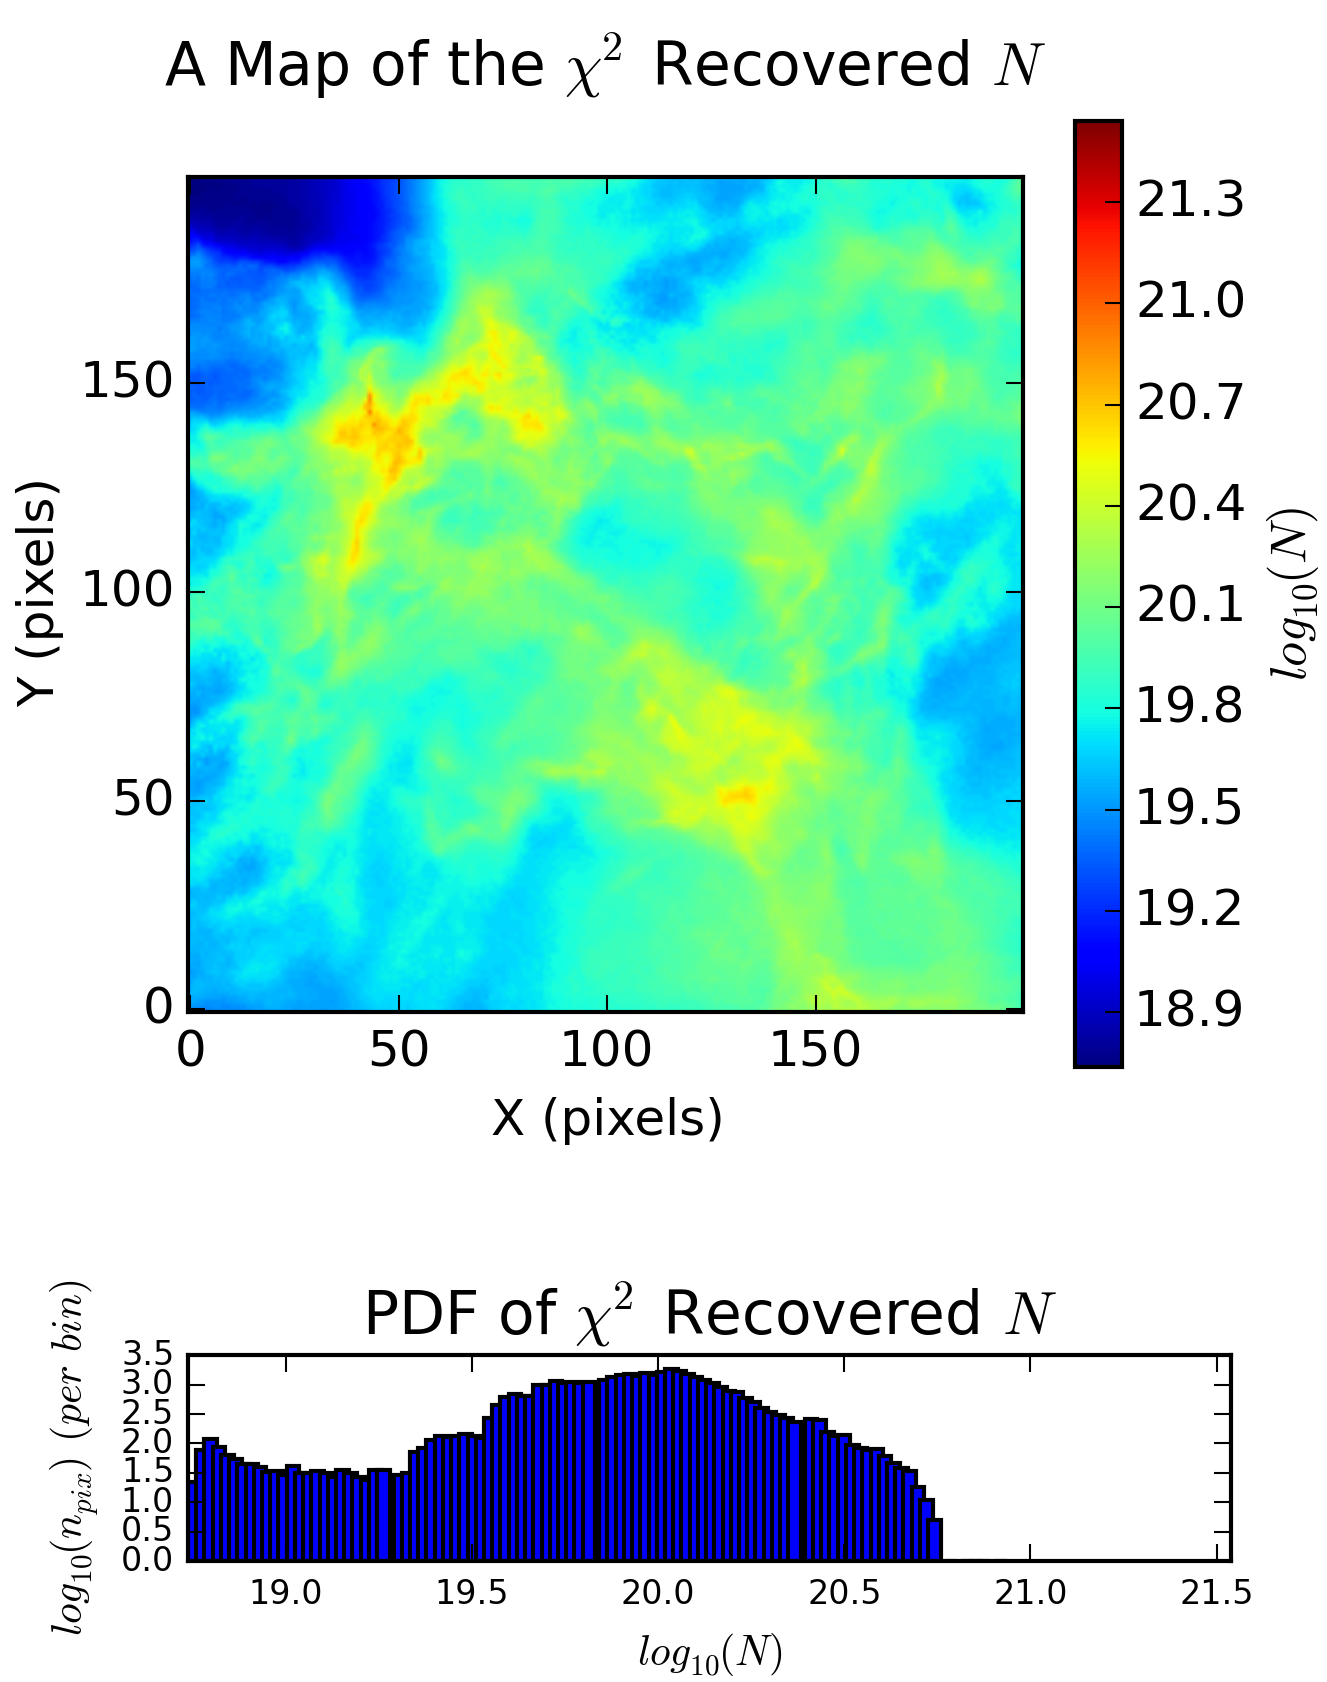
\includegraphics[width=\linewidth]{../img/sph/map_N_chi.png}
    \caption{\protect The recovered values of $N$ from the $\chi^{2}$ minimisation routine.}\label{fig:map_N_chi_sph}
    \vspace{4ex}
  \end{minipage}%%
  \begin{minipage}[b]{0.34\linewidth}
    \centering
    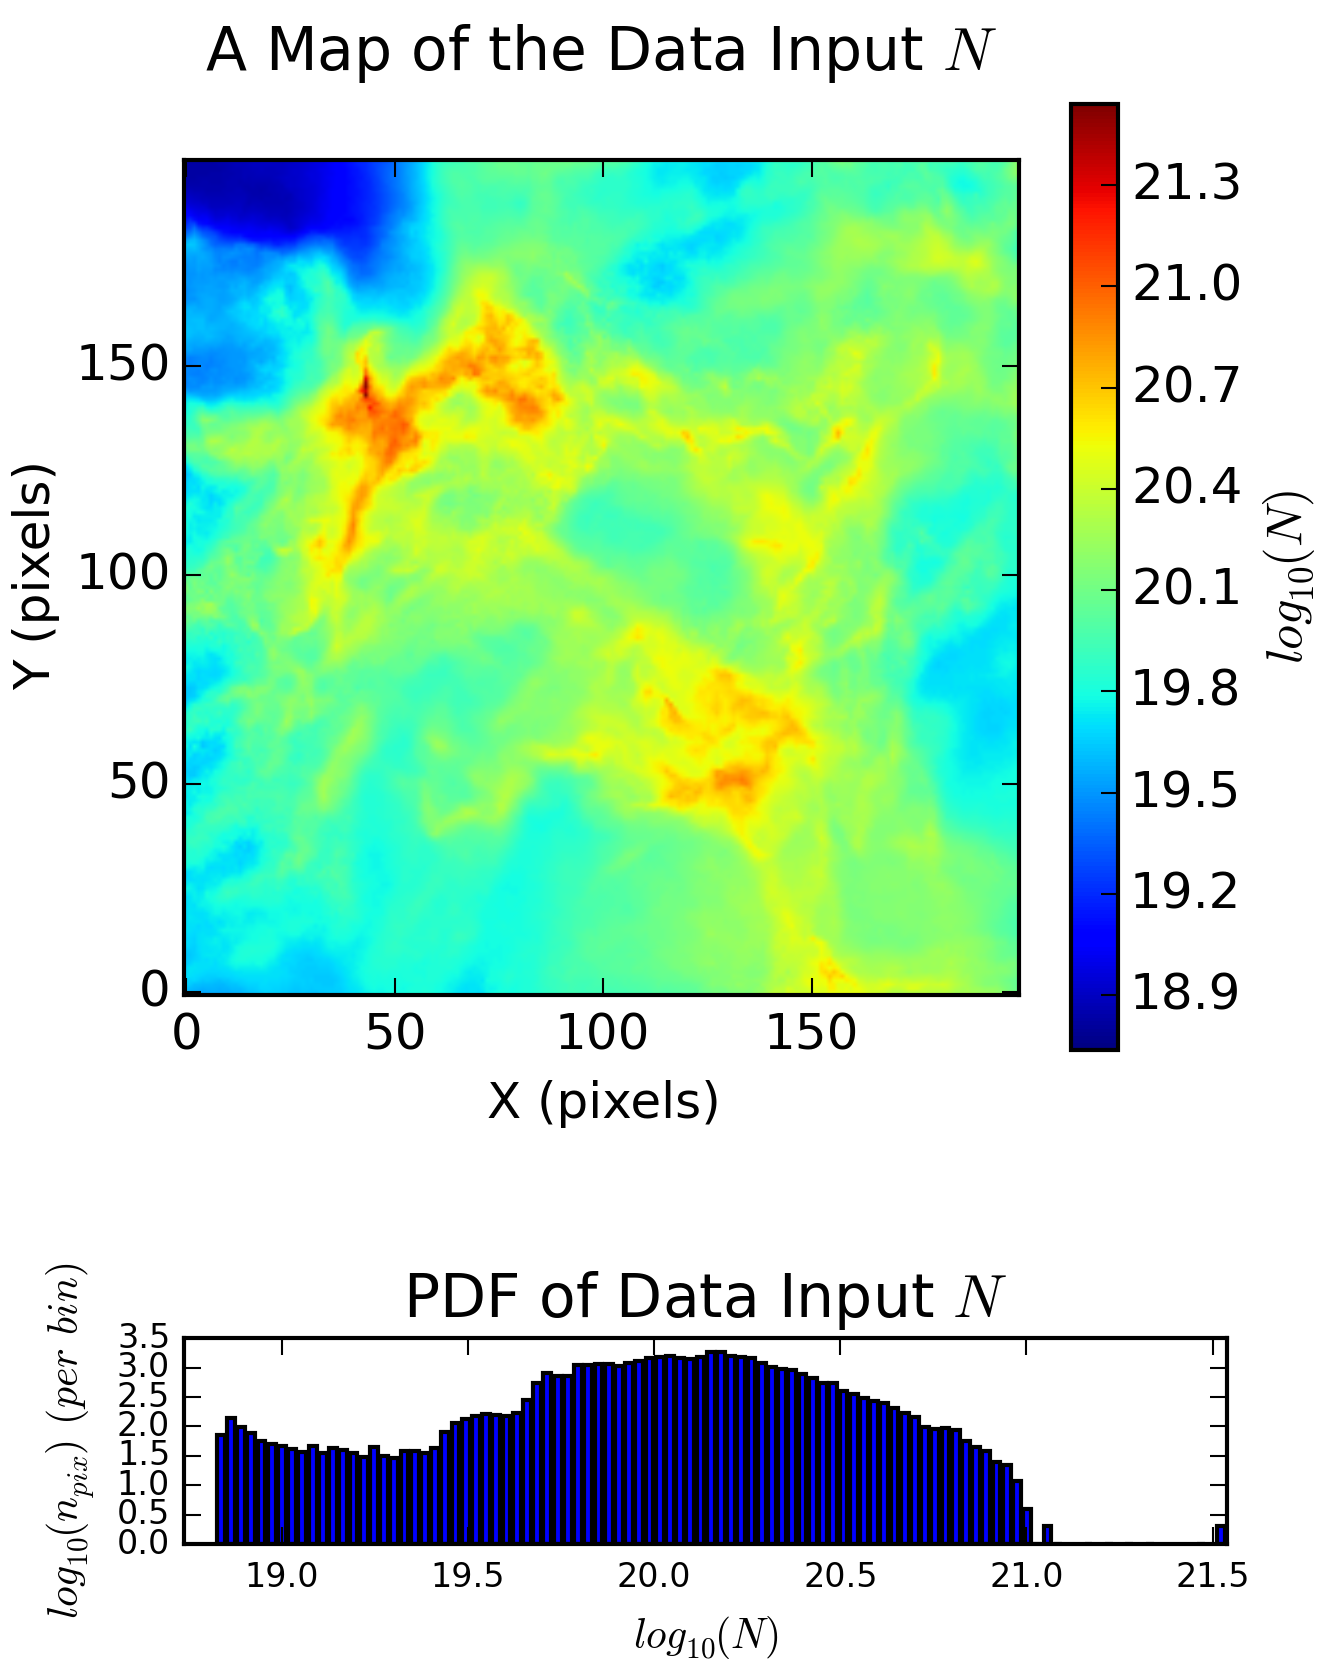
\includegraphics[width=\linewidth]{../img/sph/map_N_data.png}
    \caption{\protect The reconstructed values of $N$ from the initial input data.}\label{fig:map_N_data_sph}
    \vspace{4ex}
  \end{minipage}}
  \centerline{\begin{minipage}[b]{0.34\linewidth}
    \centering
    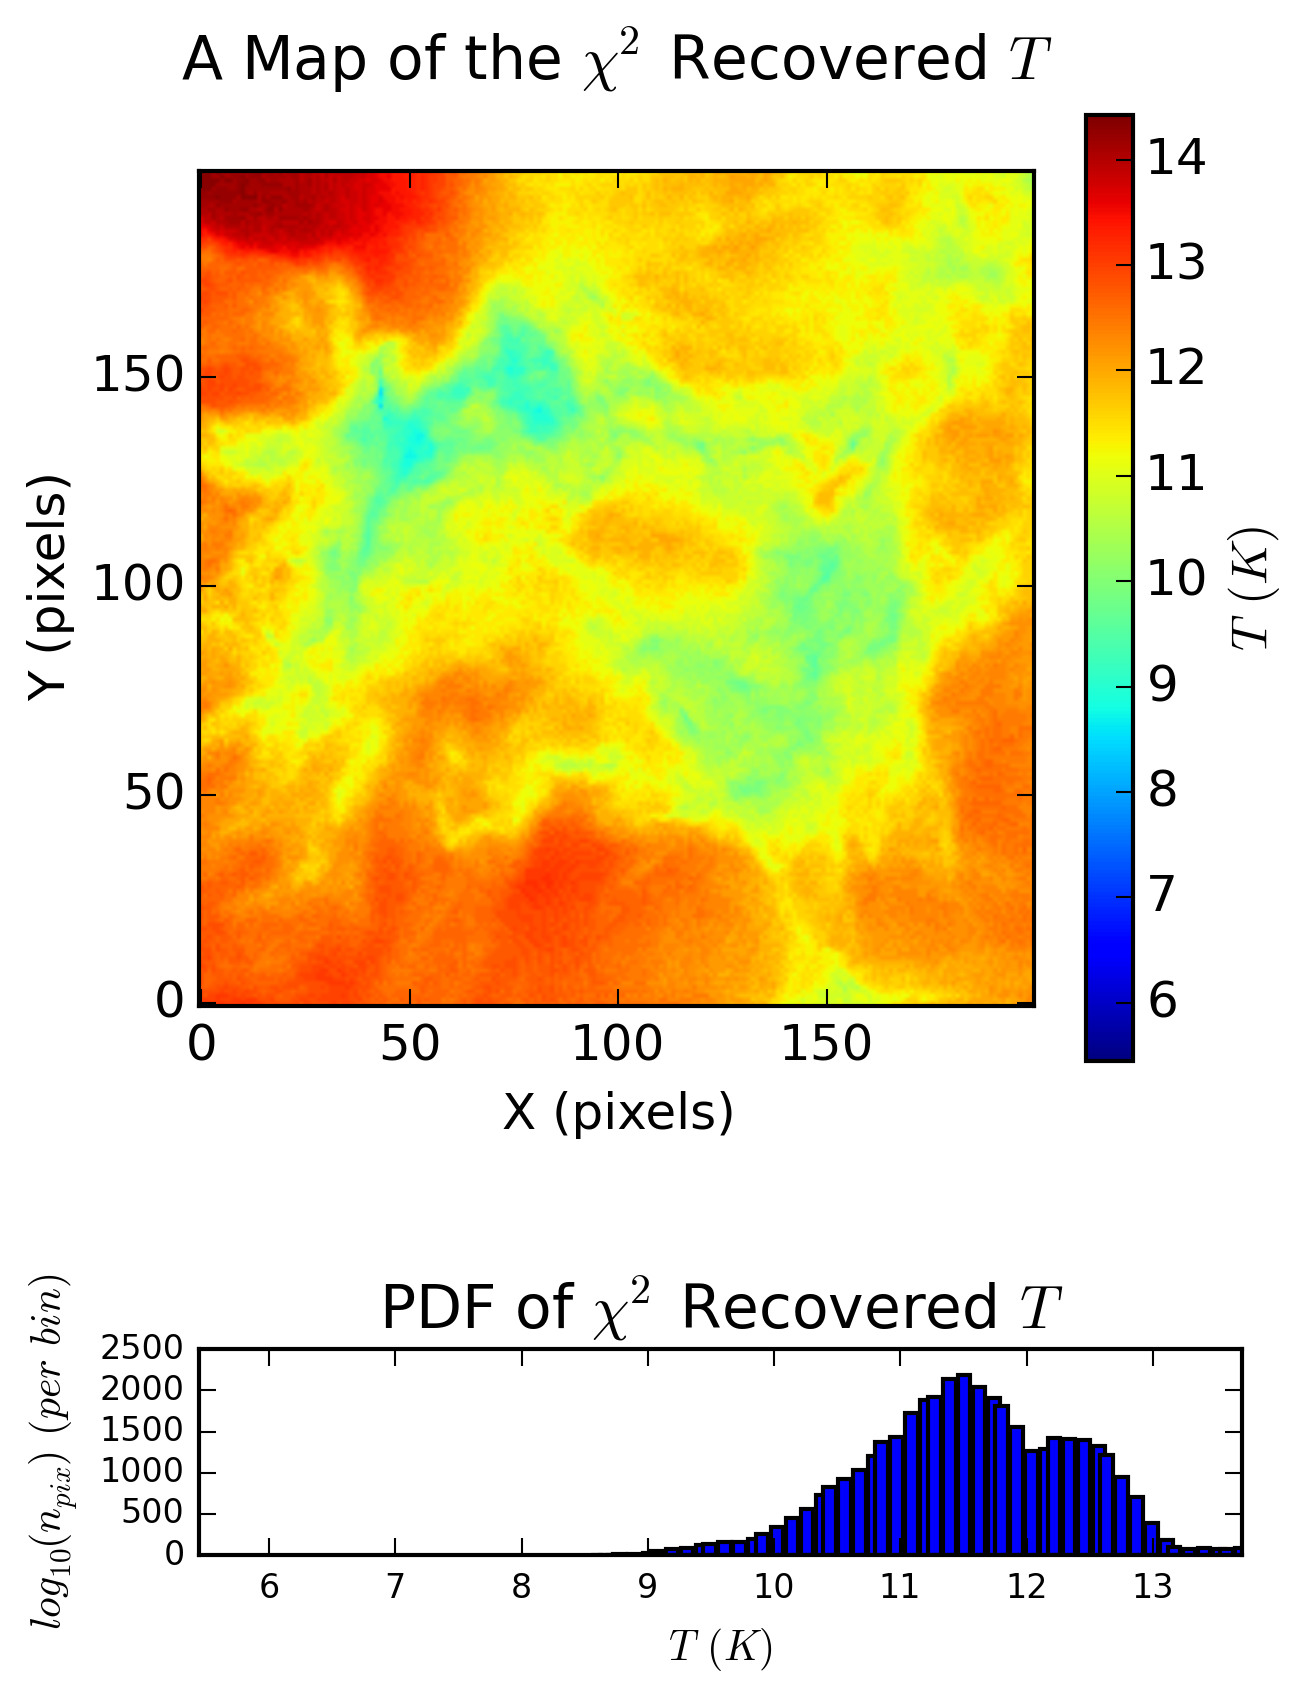
\includegraphics[width=\linewidth]{../img/sph/map_T_chi.png}
    \caption{\protect The recovered values of $T$ from the $\chi^{2}$ minimisation routine.}\label{fig:map_T_chi_sph}
    \vspace{4ex}
  \end{minipage}%%
  \begin{minipage}[b]{0.34\linewidth}
    \centering
    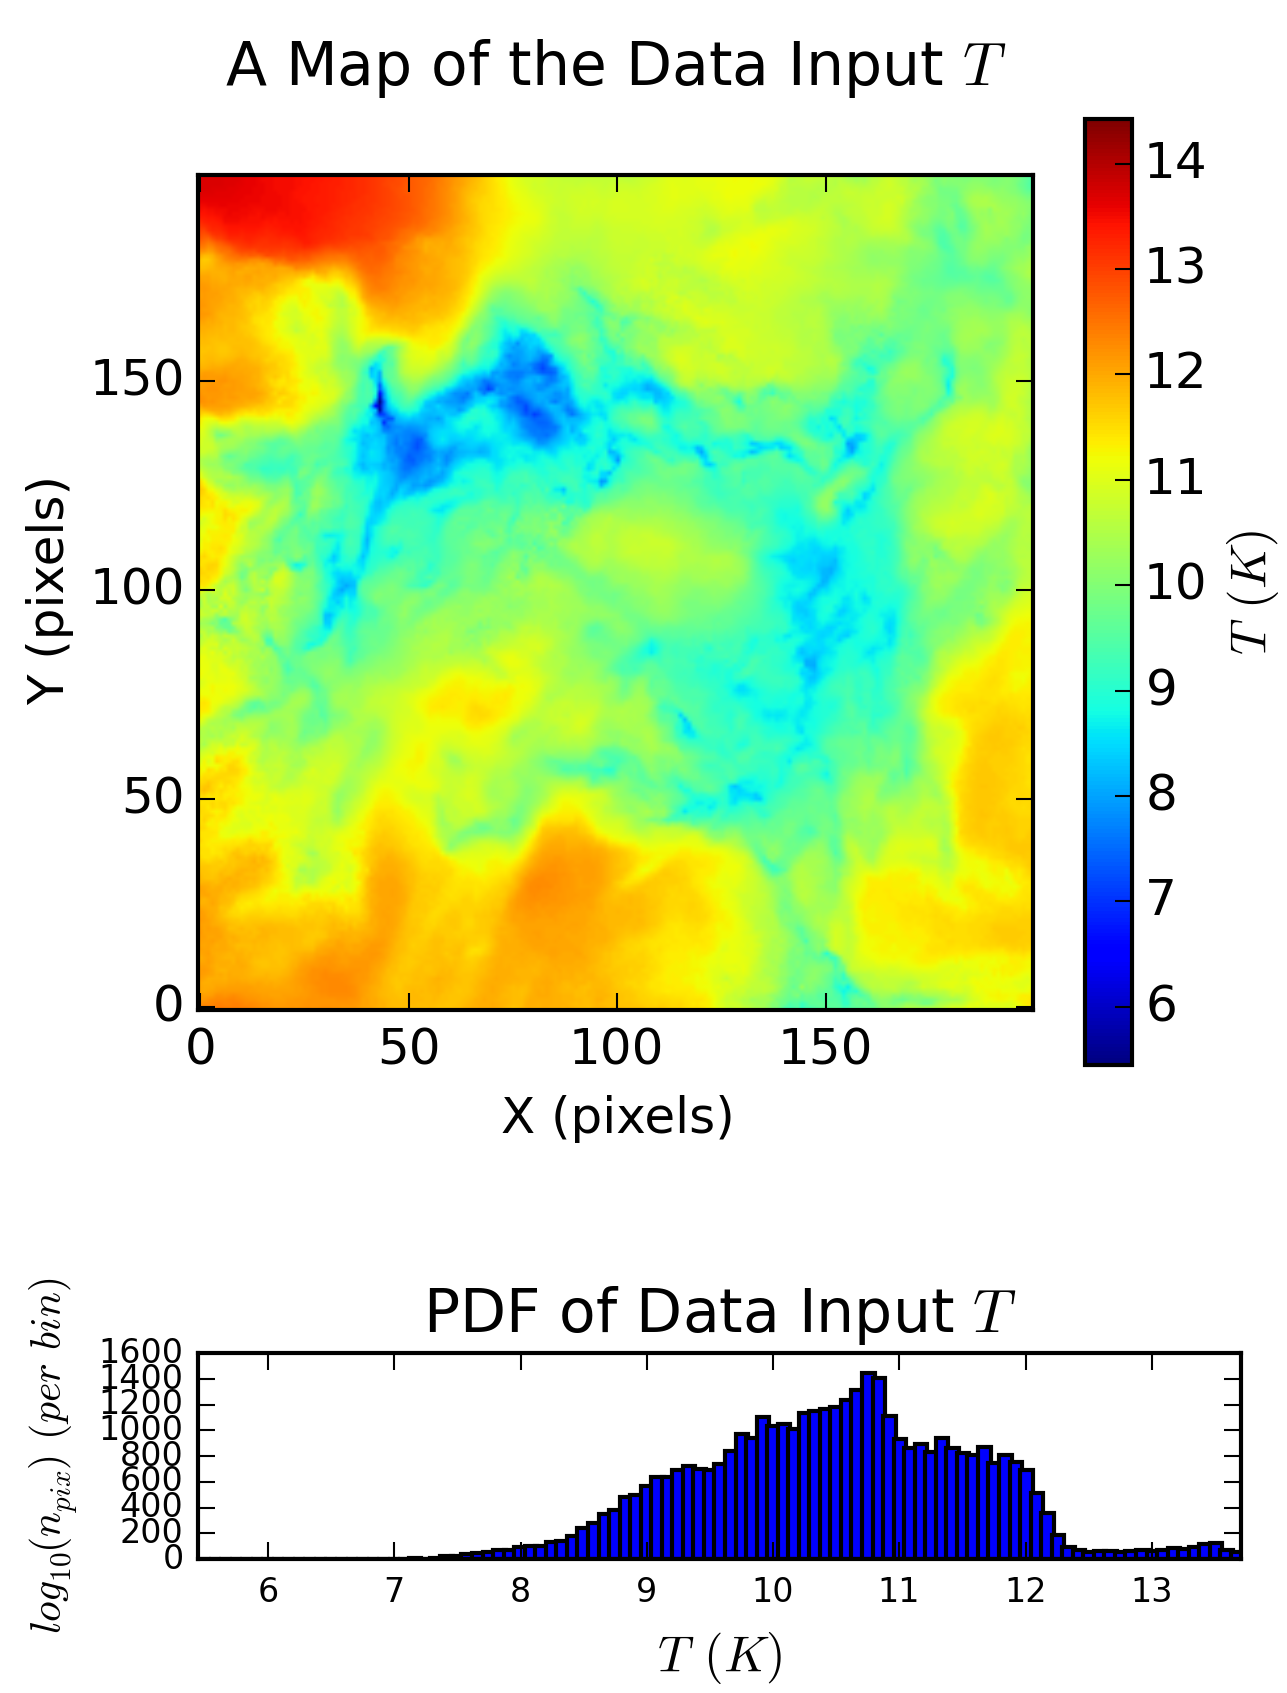
\includegraphics[width=\linewidth]{../img/sph/map_T_data.png}
    \caption{\protect The reconstructed values of $T$ from the initial input data.}\label{fig:map_T_data_sph}
    \vspace{4ex}
  \end{minipage}}
\end{figure}

\begin{figure}[H]
\minipage{0.45\textwidth}
  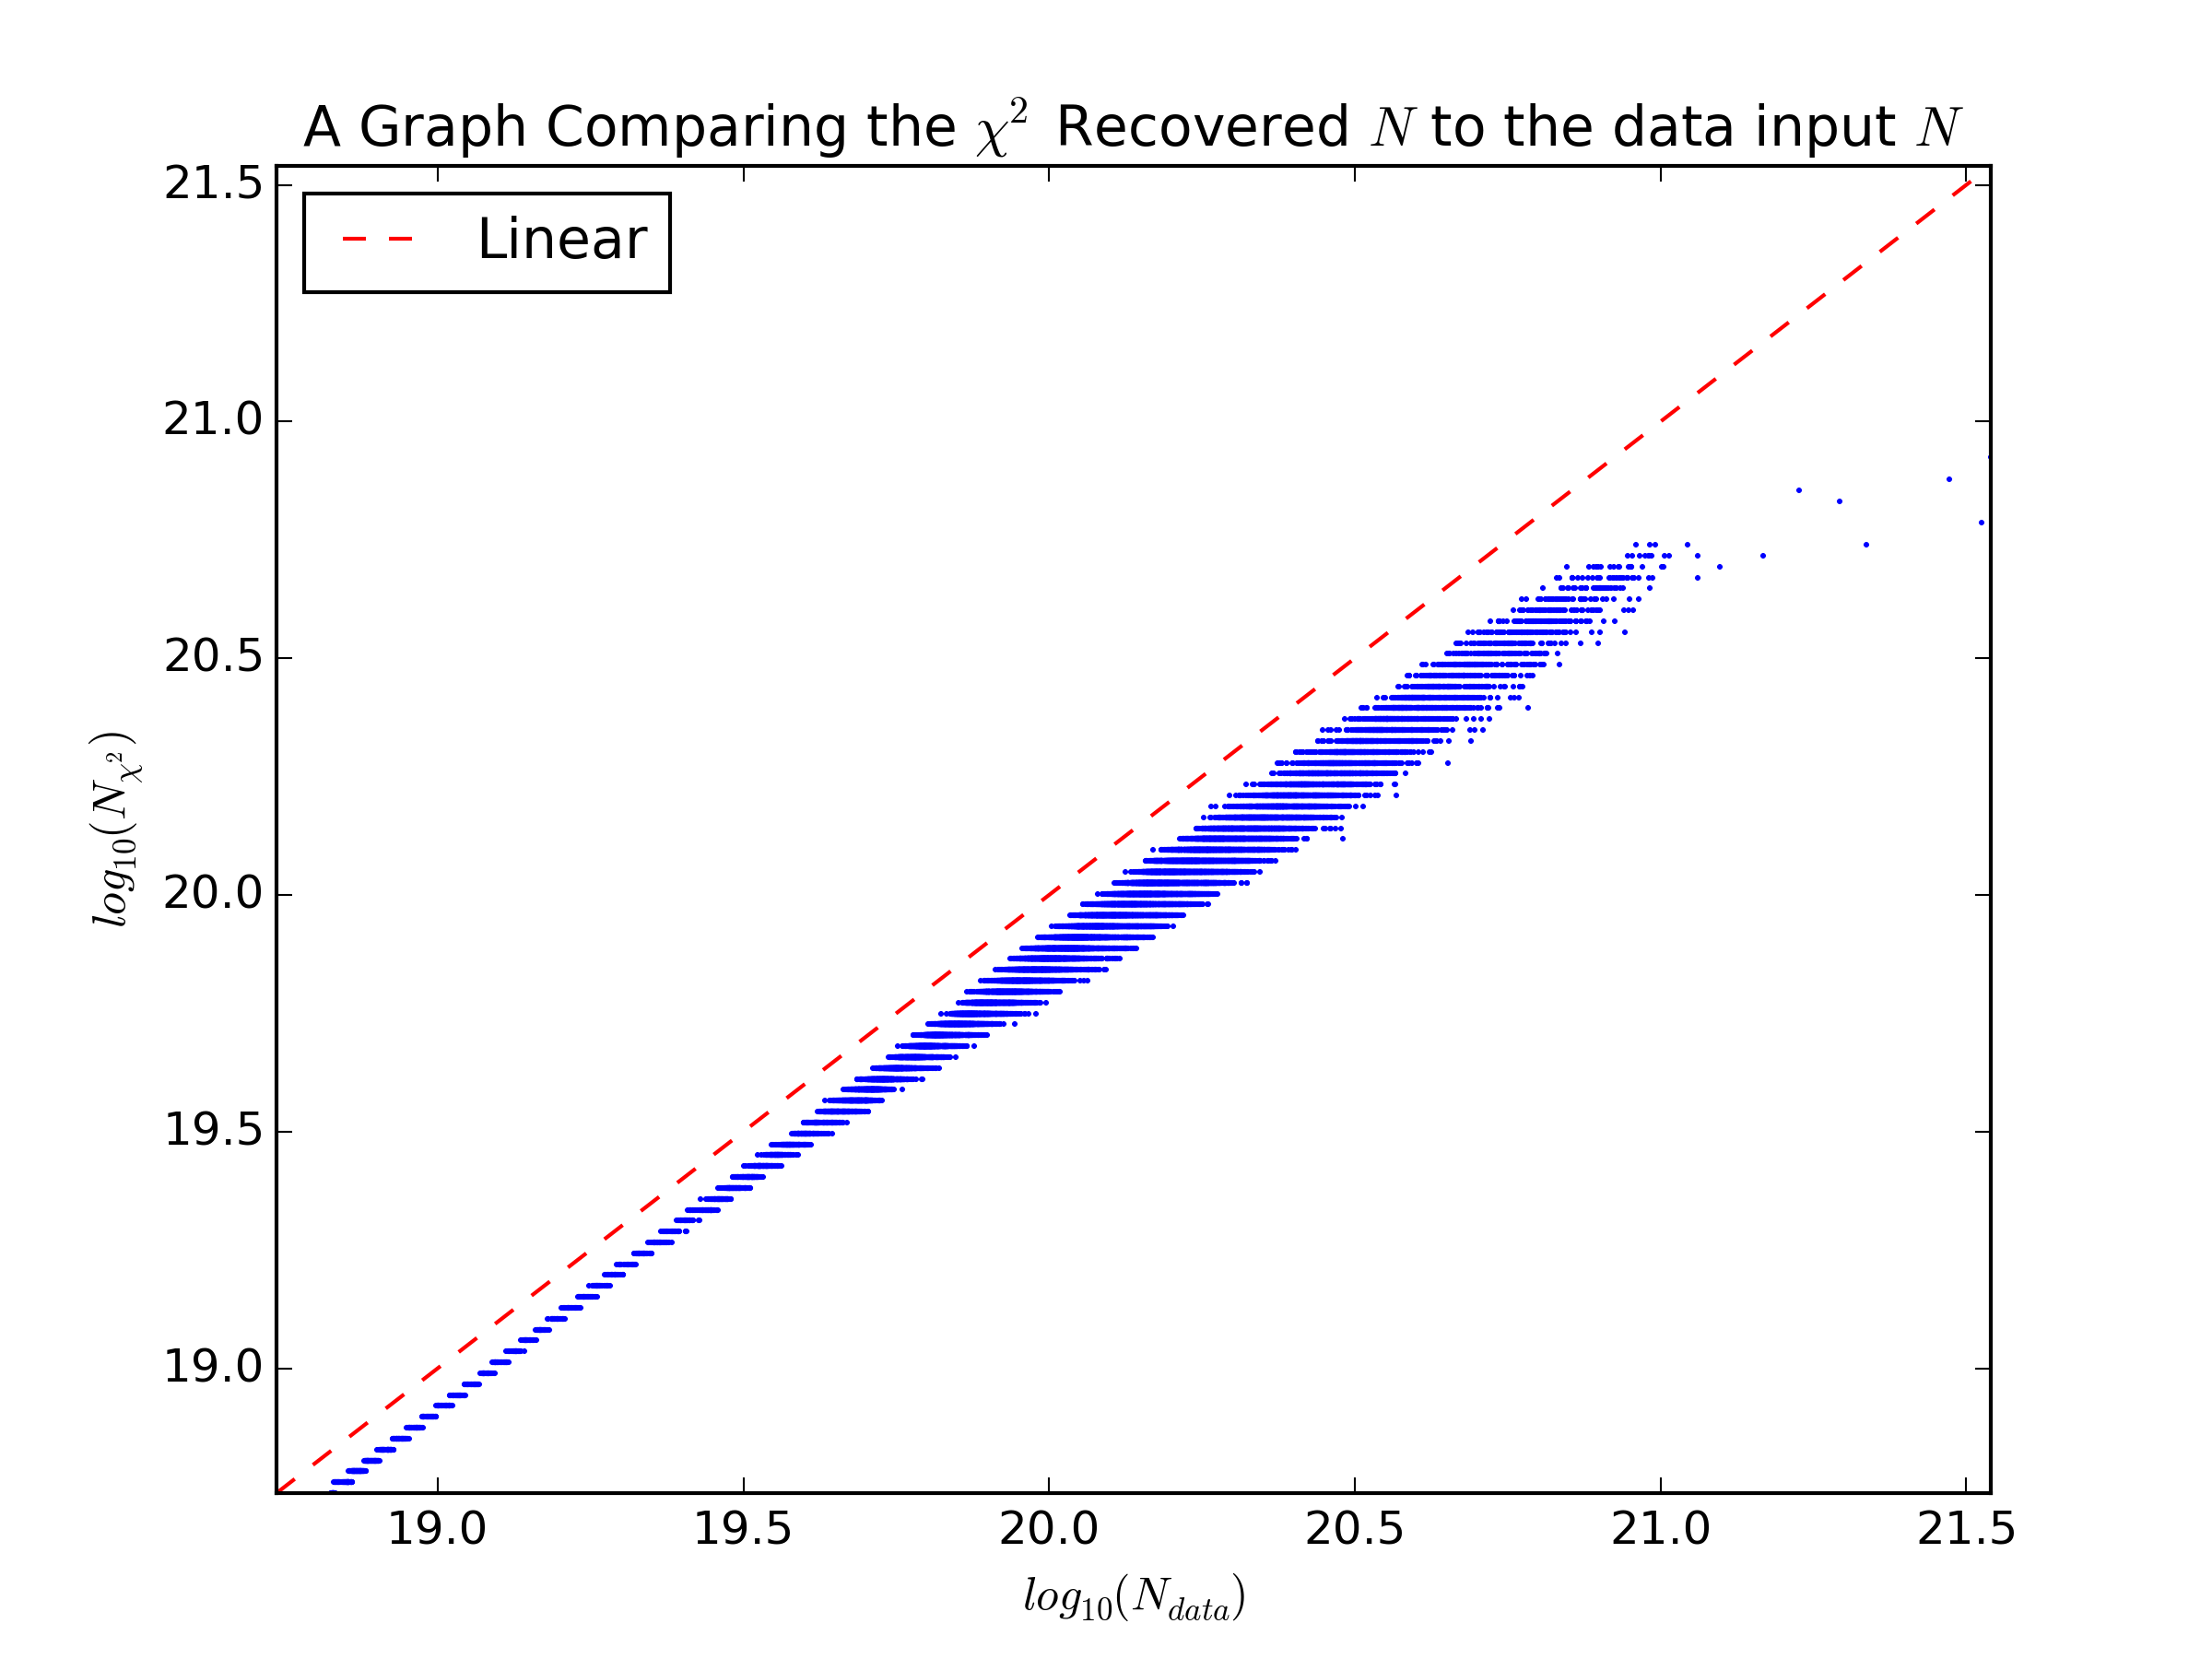
\includegraphics[width=\linewidth]{../img/sph/N.png}
  \caption{A representation of how the $\chi^{2}$ derived $N$ values compare to the initial data input $N$.}\label{fig:sph_N}
\endminipage\hfill
\minipage{0.45\textwidth}
  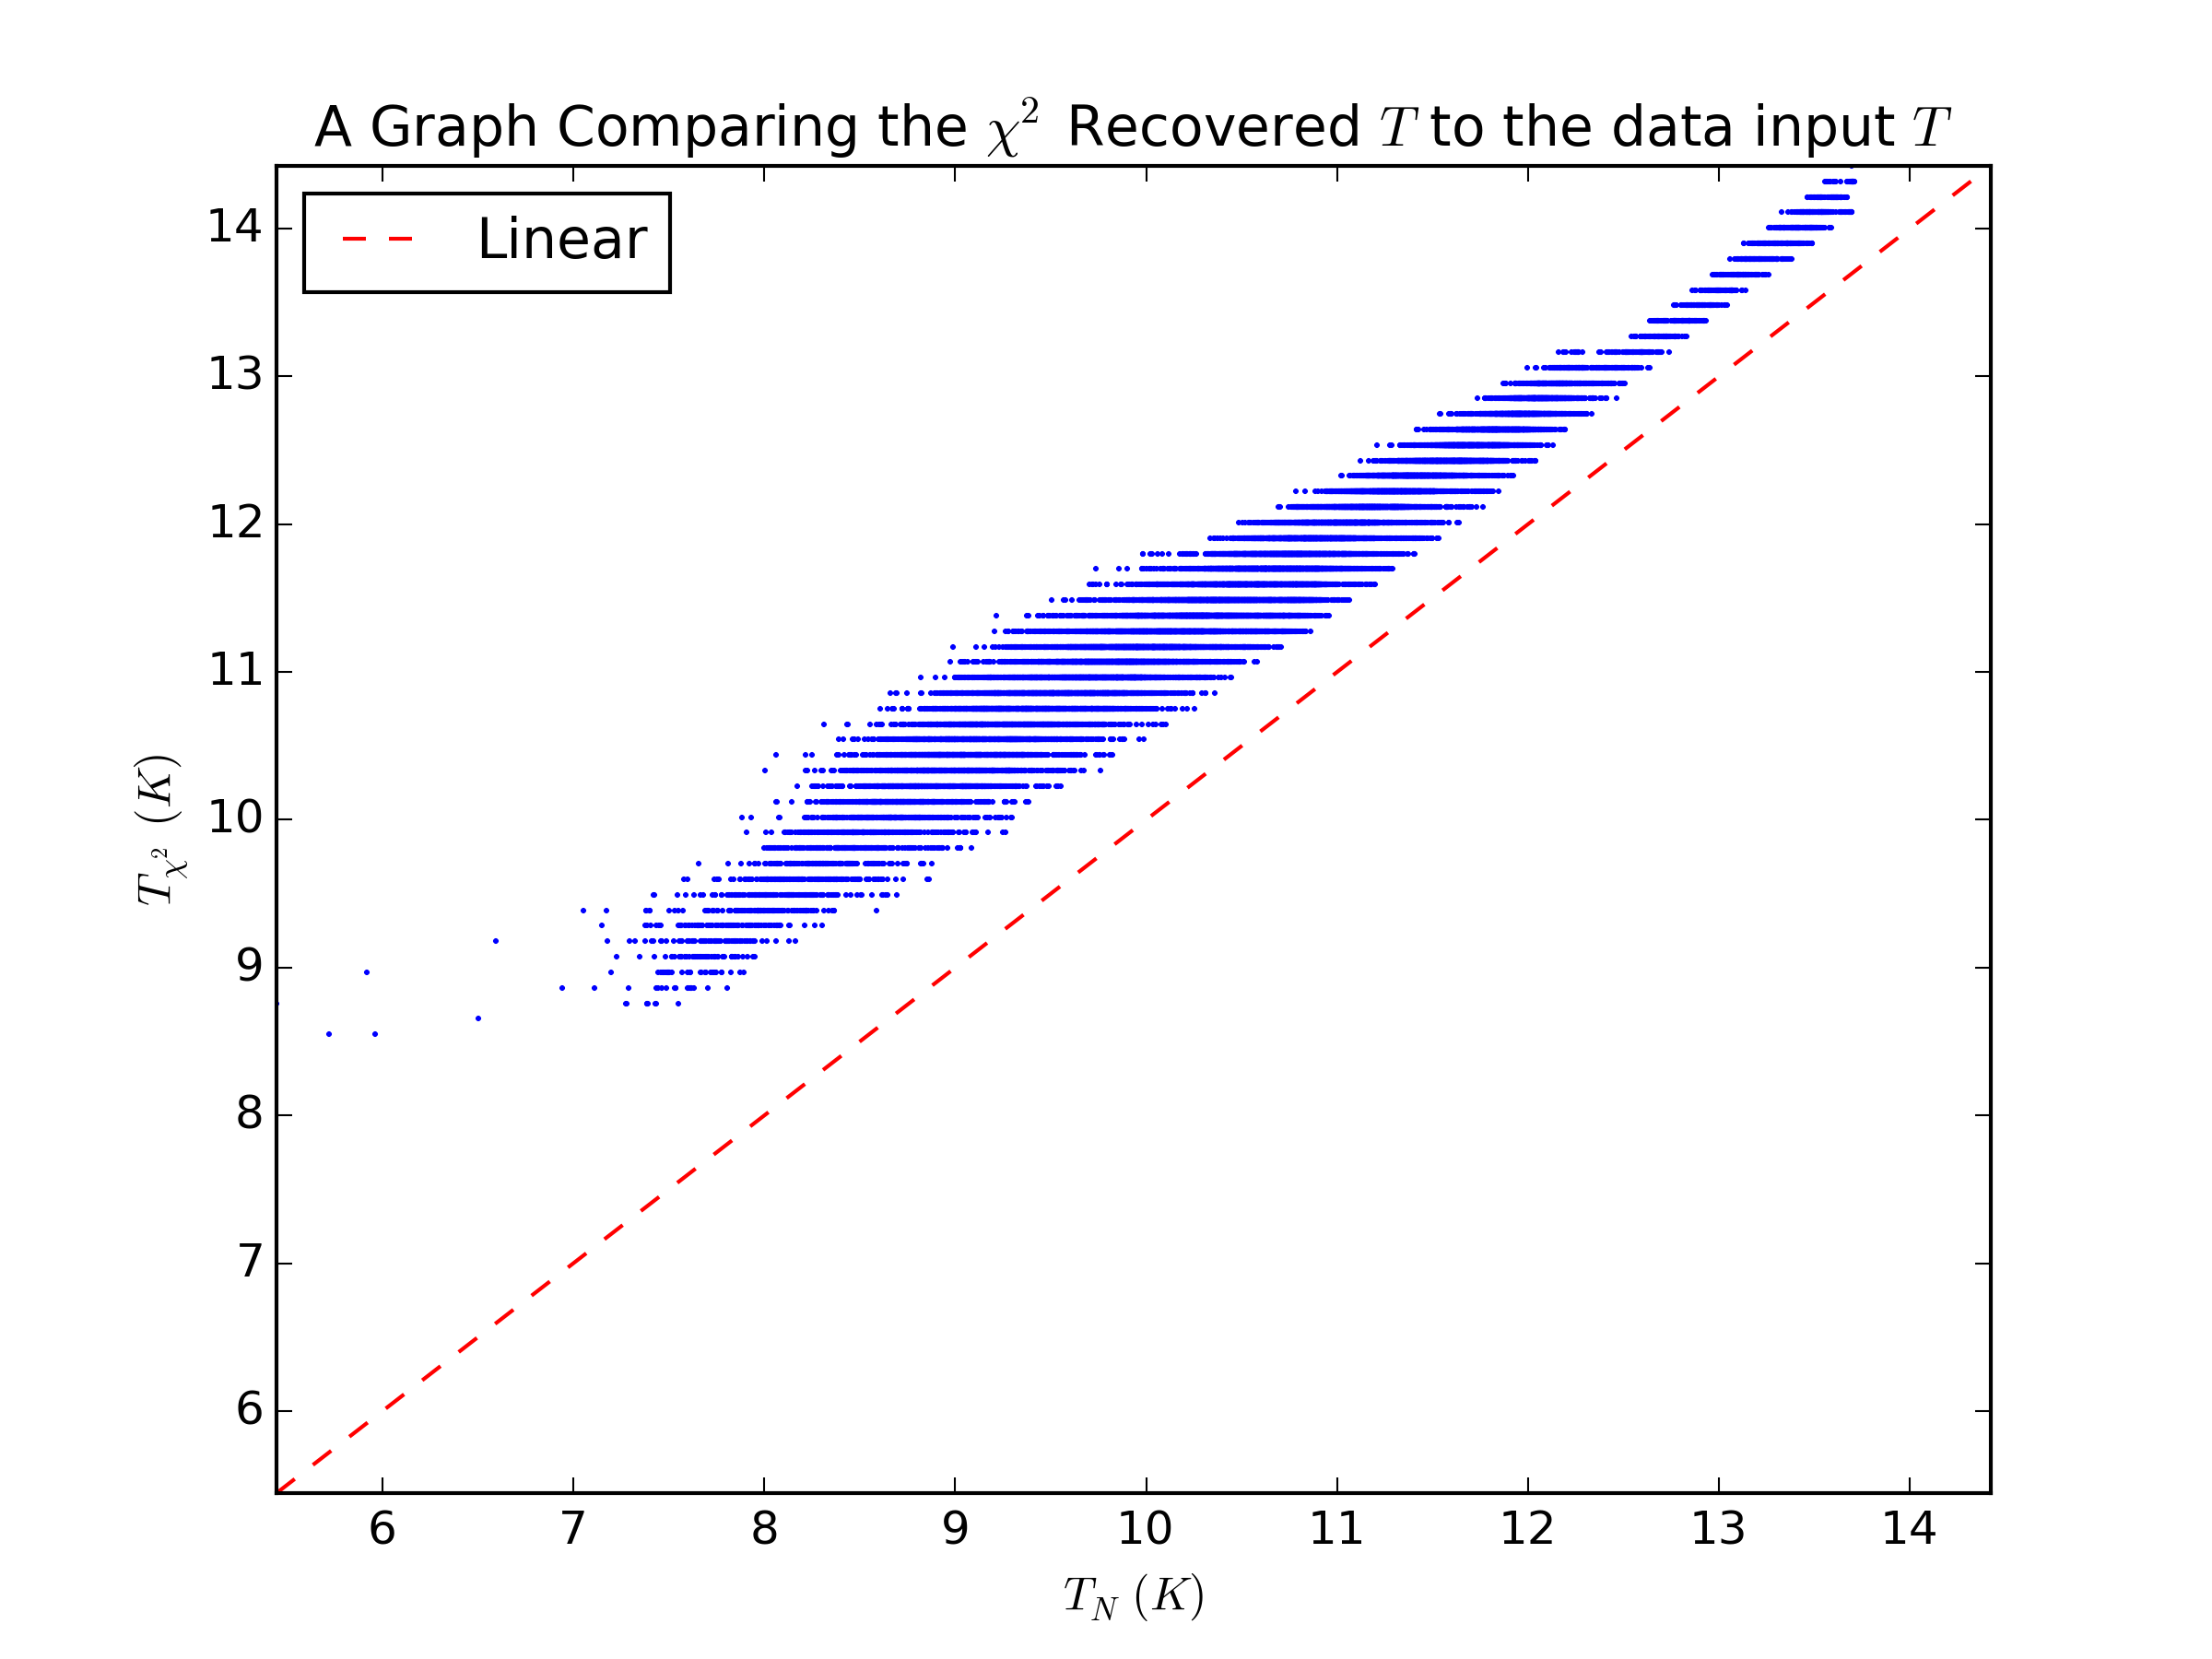
\includegraphics[width=\linewidth]{../img/sph/T.png}
  \caption{A representation of how the $\chi^{2}$ derived $T$ values compare to the initial data input $T$.}\label{fig:sph_T}
\endminipage
%\caption{A figure comparing recovered and derived values of $N$ and $T$ and how they compare. Figure \ref{fig:iso_T} shows an overestimate of the $\chi^{2}$ recovered T whilst Figure \ref{fig:iso_N} shows an underestimate the $\chi^{2}$ recovered $N$.}
\end{figure}

\begin{figure}[H]
  \centering
  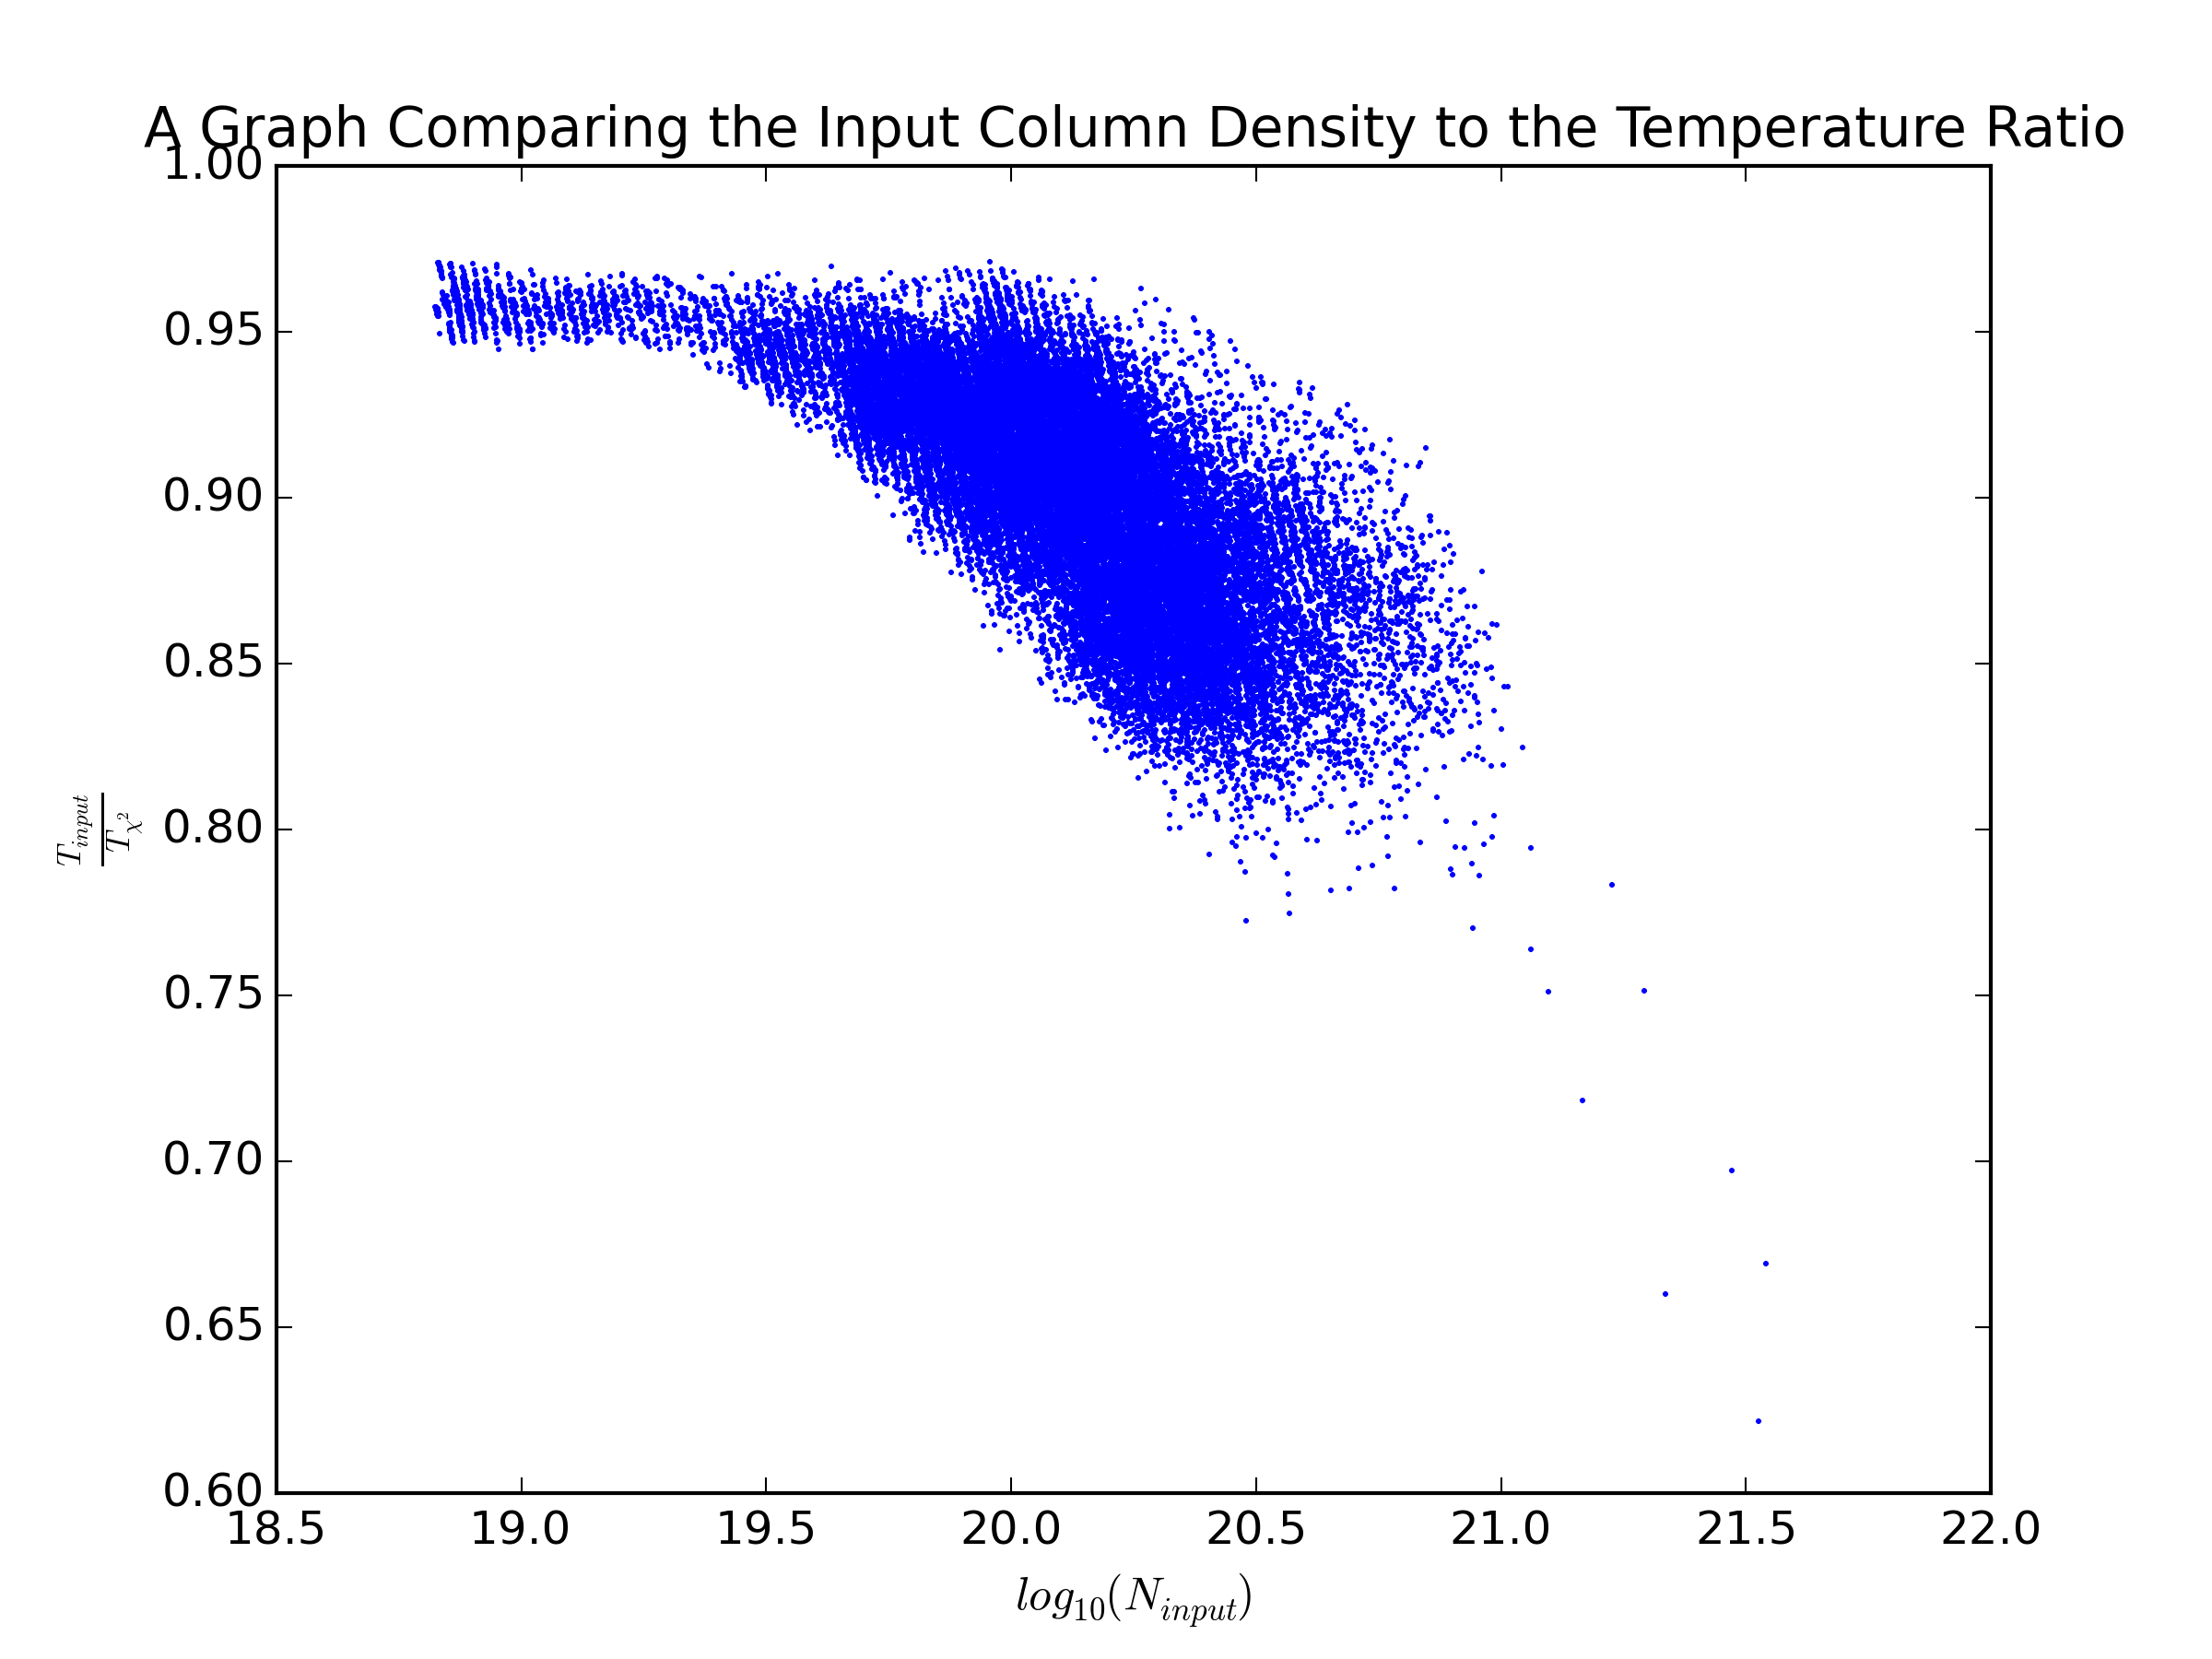
\includegraphics[width=0.45\linewidth]{../img/sph/T_ratio_inp.png}
  \caption{A plot showing how the ratio of $T_{input}/T_{\chi^{2}}$ varies with the data derived $N$.}\label{fig:T_ratio_sph}
%\caption{A figure comparing recovered and derived values of $N$ and $T$ and how they compare. Figure \ref{fig:iso_T} shows an overestimate of the $\chi^{2}$ recovered T whilst Figure \ref{fig:iso_N} shows an underestimate the $\chi^{2}$ recovered $N$.}
\end{figure}

We notice here, owing to the more intricate structure within the image, that $\chi^{2}$ minimisation recovers the majority of that structure, despite failing to recover a number of obvious high density regions. Of particular interest here is the small peak at $log_{10}(N)=21.5$ that the $\chi^{2}$ routine fails to detect. Similarly to the isothermal case in Figure \ref{fig:map_N_chi}, these values are underestimated to a small degree relative to the data derived $N$, as shown by the distribution existing further towards low $N$ in the $\chi^{2}$ case. We also note that far less of the higher $N$ material is recovered, as evidenced by the maximum of the $\chi^{2}$ $N$ PDF falling below that of the data derived $N$; data derived $N$ extends continuously to $log_{10}(N)=21$, whilst the $\chi^{2}$ continues to $log_{10}(N)=20.7$. However, the shape of the PDFs remain largely intact, similar to the isothermal case. One feature that is emergent here and not in the isothermal sphere however is the sharp peak in $log_{10}(n_{pix})$ at small $N$ in both $\chi^{2}$
$N$ and data derived $N$. This highlights the relative abundance of low column material within the image. The PDF also features an extended `tail` such that the expected lognormal form is departed from at both low $N$ as well as high $N$. In the high $N$ case the `tail` is best described by a power-law relation \parencite{tail,powerlaw}. It is widely accepted that this power-law indicates the presence of gravitationally bound material.

Figures \ref{fig:map_T_chi_sph} and \ref{fig:map_T_data_sph} illustrate that, again like the isothermal case, $\chi^{2}$ $T$ is overestimated relative to the data derived $T$. Also apparent is the fact that the $\chi^{2}$ minimisation fails to recover a lot of the colder material in the image, as evidenced from the minimum of the $\chi^{2}$ $T$ PDF beginning above that of the data derived $T$ PDF. Similar to the isothermal case, the shape of the PDFs remains consistent between $\chi^{2}$ and data derived.

Figures \ref{fig:sph_N} and \ref{fig:sph_T} show how data derived quantities varies with the $\chi^{2}$ recovered quantity. The linear reference line is plotted as a red line. Figure \ref{fig:sph_N} shows that the $\chi^{2}$ recovered $N$ is now consistently underestimated with respect to the data derived $N$ as shown by the data existing under the linear relationship line. This relationship is, however, linear in log space at low $N$ though the disparity increases at higher data derived $N$. The scatter in data derived $N$ that produces the same value of $\chi^{2}$ $N$ increases towards the middle of the data. Interestingly, this linear relationship is departed from at high $N$ as evidenced by the data points falling away from the main grouping (and further away from the linear relationship line). Figure \ref{fig:sph_T} shows the inverse relationship in
$T$: the $\chi^{2}$ $T$ is now largely overestimated relative to the data derived $T$, though this overestimate is much larger at low data derived $T$. The same departure in datapoints is observed at low data derived $T$ in this case (as opposed to high data derived quantity as was the case in Figure \ref{fig:sph_N}).

Figure \ref{fig:T_ratio_sph} displays how the ratio of the determined temperatures $T_{input}/T_{\chi^{2}}$ varies with the data derived $N$. It clearly shows that as the data derived $N$ increases the $\chi^{2}$ recovered $T$ is increasingly overestimated. Of note here is the fact that even in the low $N$ regime, the $\chi^{2}$ recovered $N$ remains overestimated. This relationship continues into the high $N$ regime, culiminating in a sharp drop off that shows the $\chi^{2}$ recovered $T$ is almost 3 times the data derived $T$.
Figure \ref{fig:T_ratio_sph} also shows a large degree of scatter that increases with $N$, implying that not only can multiple different $N$ values produce the same estimate of $T_{\chi^{2}}$ but also that this scatter increases as $N$ increases. To further illustrate this, Figure \ref{fig:contours} shows how the $\chi^{2}$ recovered values of $N$ and $T$ compare.

\begin{figure}[H]
  \centering
  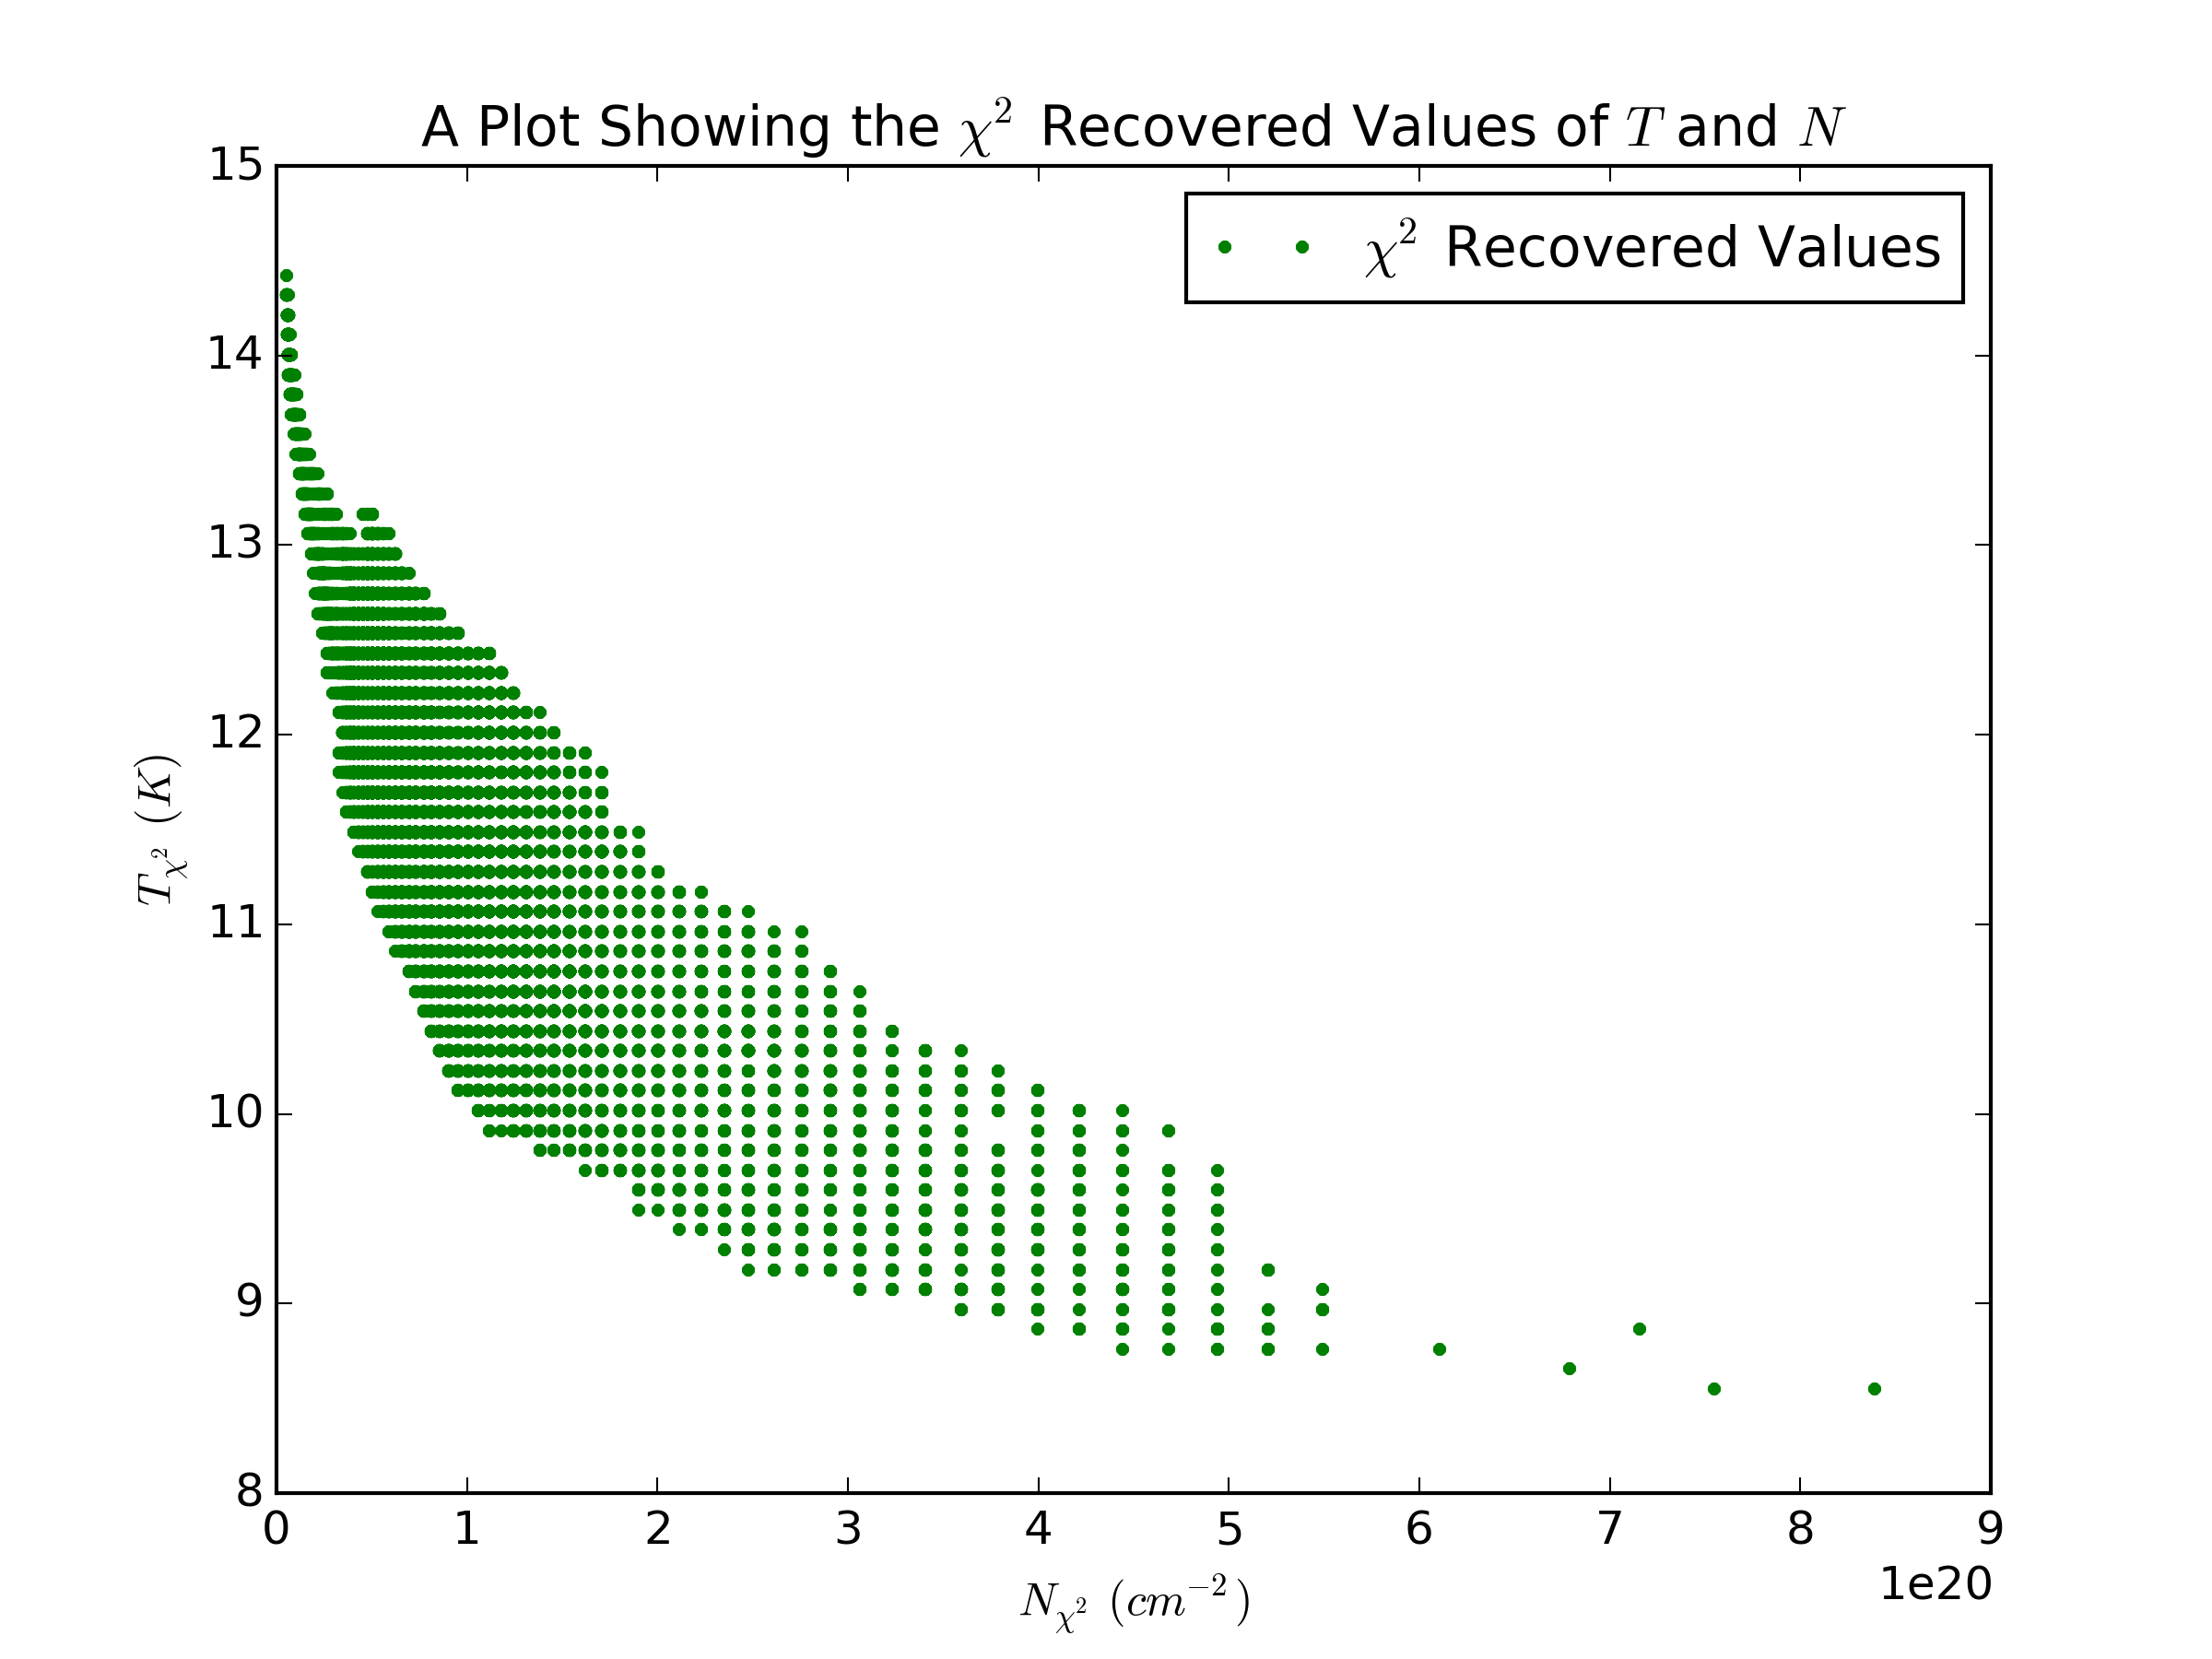
\includegraphics[width=0.5\linewidth]{../img/sph/contours.png}
  \caption{A plot showing the relationship between the $\chi^{2}$ recovered values of $N$ and $T$.}\label{fig:contours}
%\caption{A figure comparing recovered and derived values of $N$ and $T$ and how they compare. Figure \ref{fig:iso_T} shows an overestimate of the $\chi^{2}$ recovered T whilst Figure \ref{fig:iso_N} shows an underestimate the $\chi^{2}$ recovered $N$.}
\end{figure}

Figure \ref{fig:contours} exhibits an elliptical shape, such that minimal scatter is observed in the minima and maxima of $T$ and $N$. The largest scatter occurs in the centre of the data, where single $T$ provides multiple differing values of $N$. Likewise, single $N$ can provide multiple different values of $T$. A similar relationship is observed in \textcite{noise,noiseb} for $\beta$ and $T$, who attribute the elliptical data to be a result of noise in the observations.

\section{Line of sight temperature variations}
Figures \ref{fig:iso_N}, \ref{fig:iso_T},  \ref{fig:sph_T}, \ref{fig:sph_N} as well as Figure \ref{fig:contours} highlight underestimates of $N$ and overestimates of $T$ in the $\chi^{2}$ minimisation test.
Figures \ref{fig:iso_los} and \ref{fig:sph_los} show the line of sight temperature variations $\sigma^{2}$ as a function of the data derived $N$ and $T$. The line of sight temperature variation is expressed as the standard deviation of the weighted mean temperature expressed in Equation \ref{eq:los}.

\begin{figure}[H]
\minipage{0.45\textwidth}
  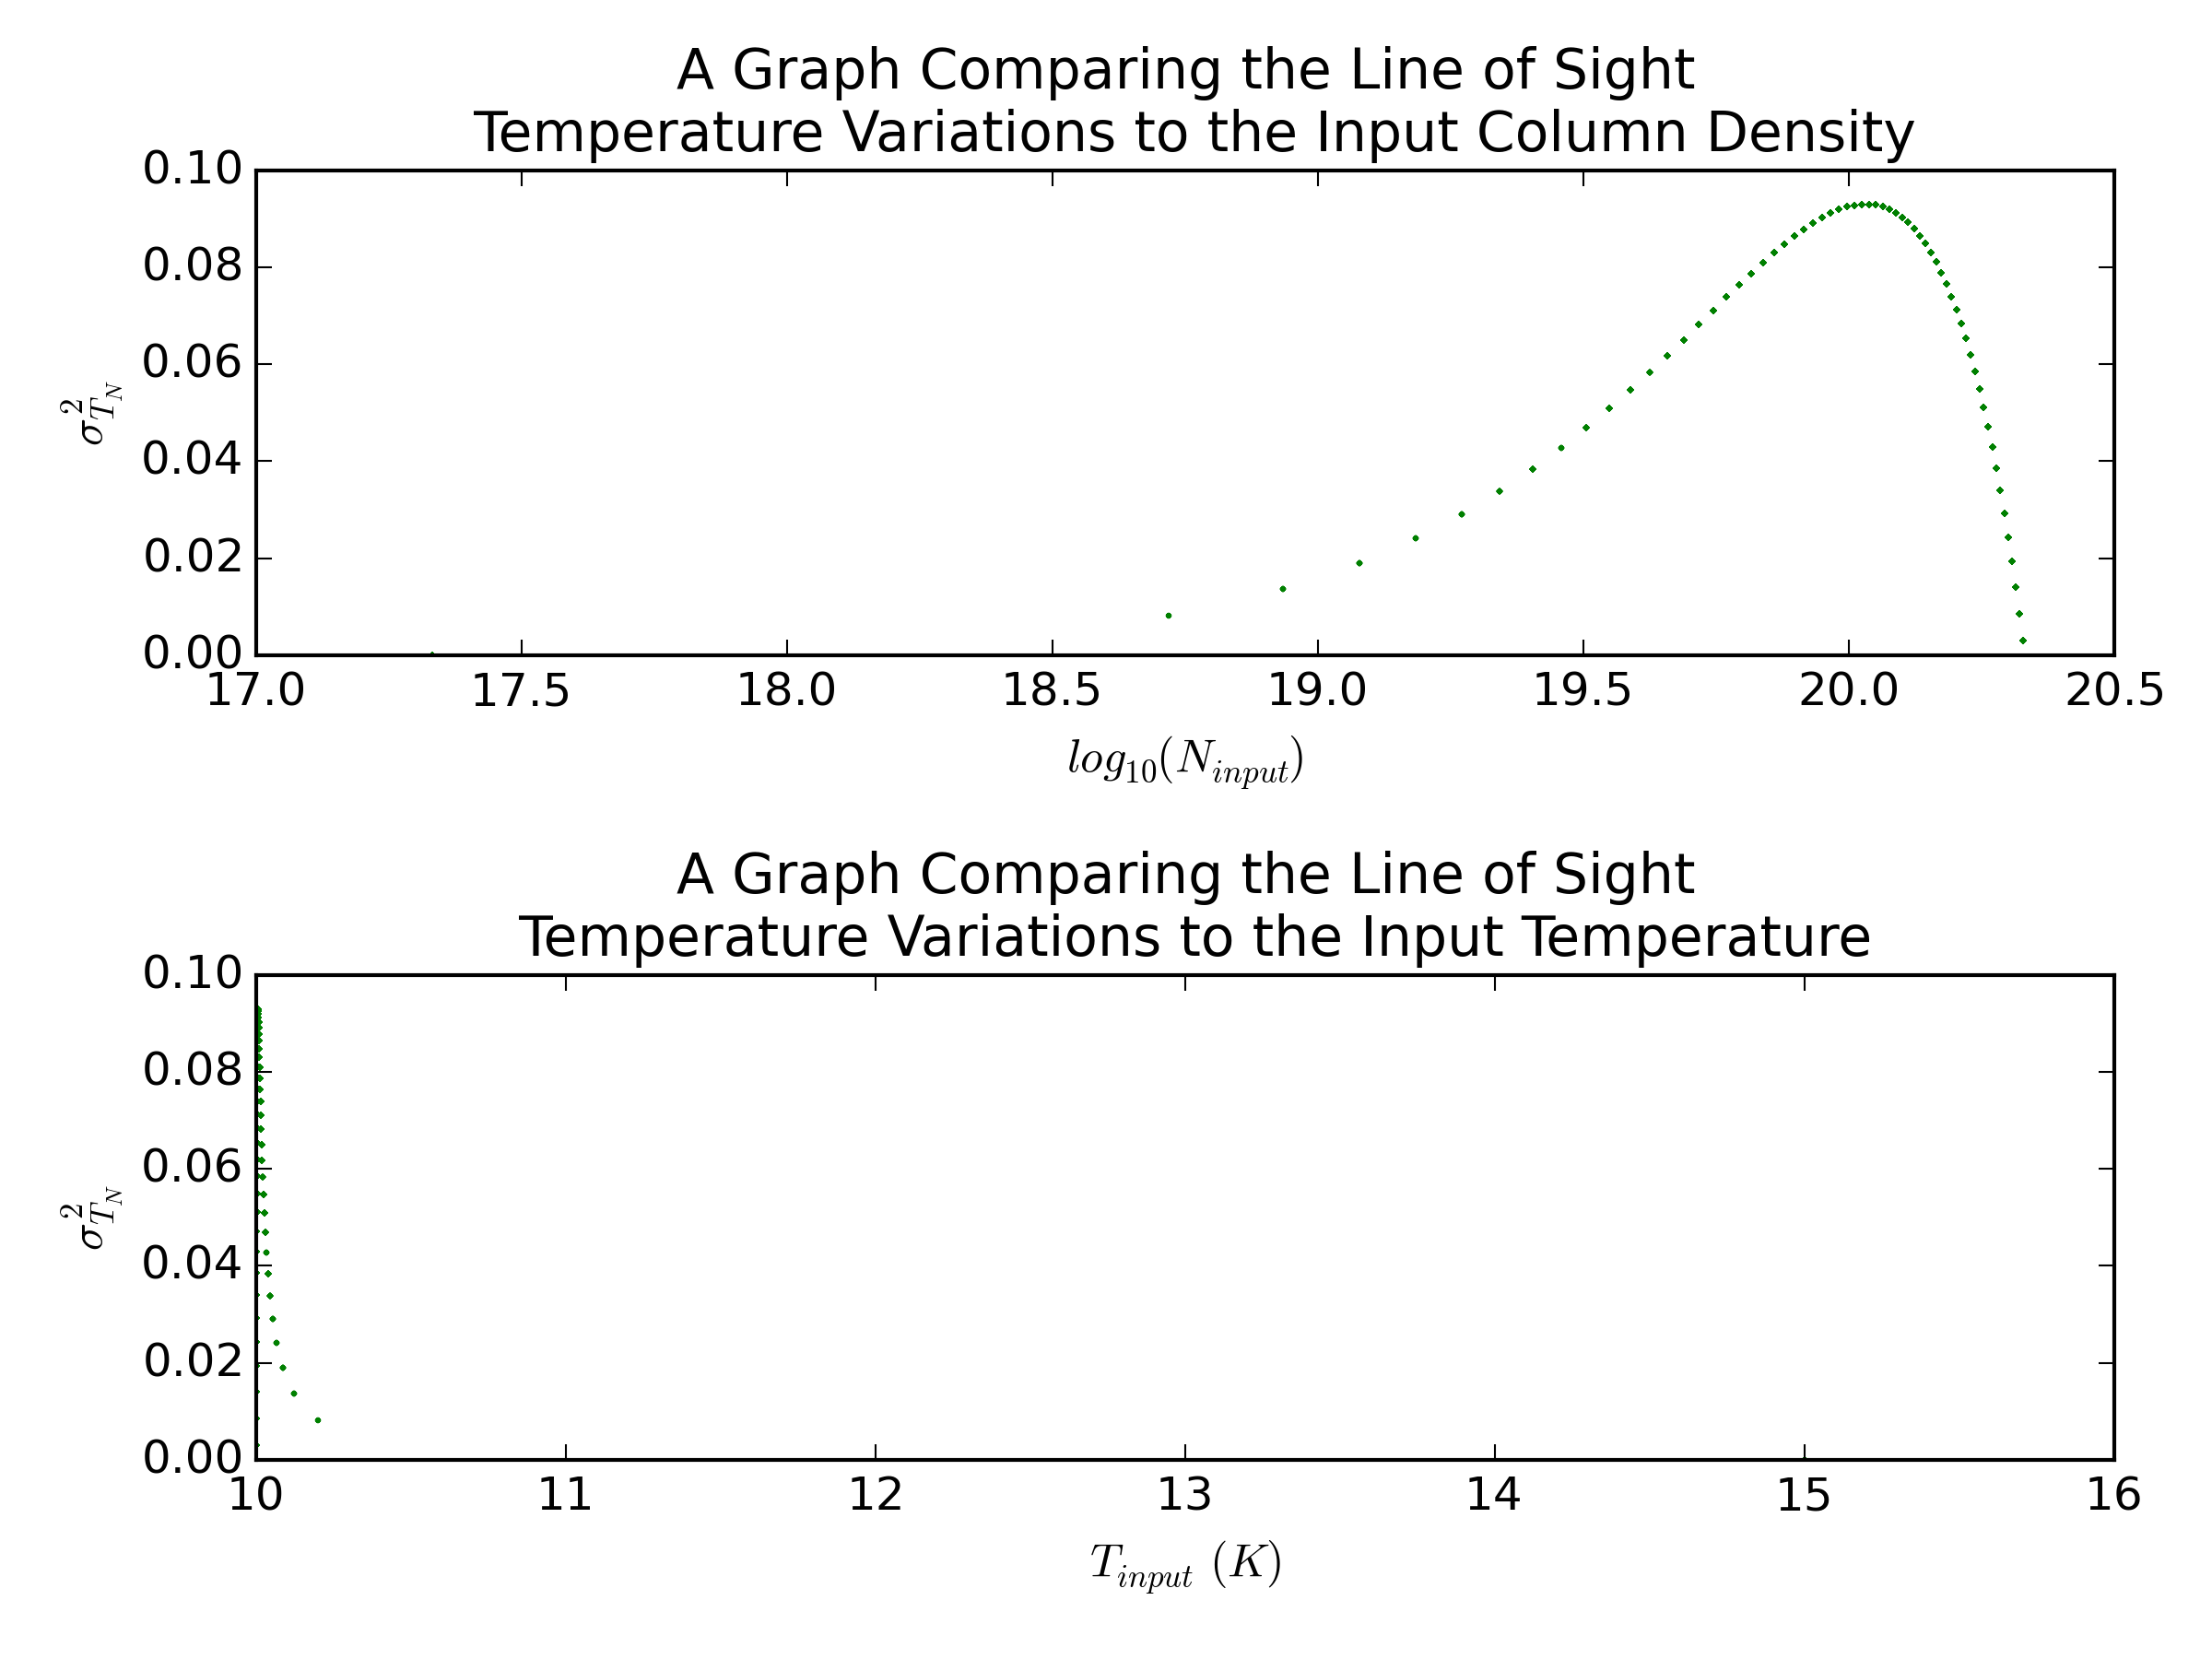
\includegraphics[width=\linewidth]{../img/sim/sigma_T_inp.png}
  \caption{The line of sight temperature variations in the isothermal sphere case as a function of the data derived $N$ and $T$.}\label{fig:iso_los}
\endminipage\hfill
\minipage{0.45\textwidth}
  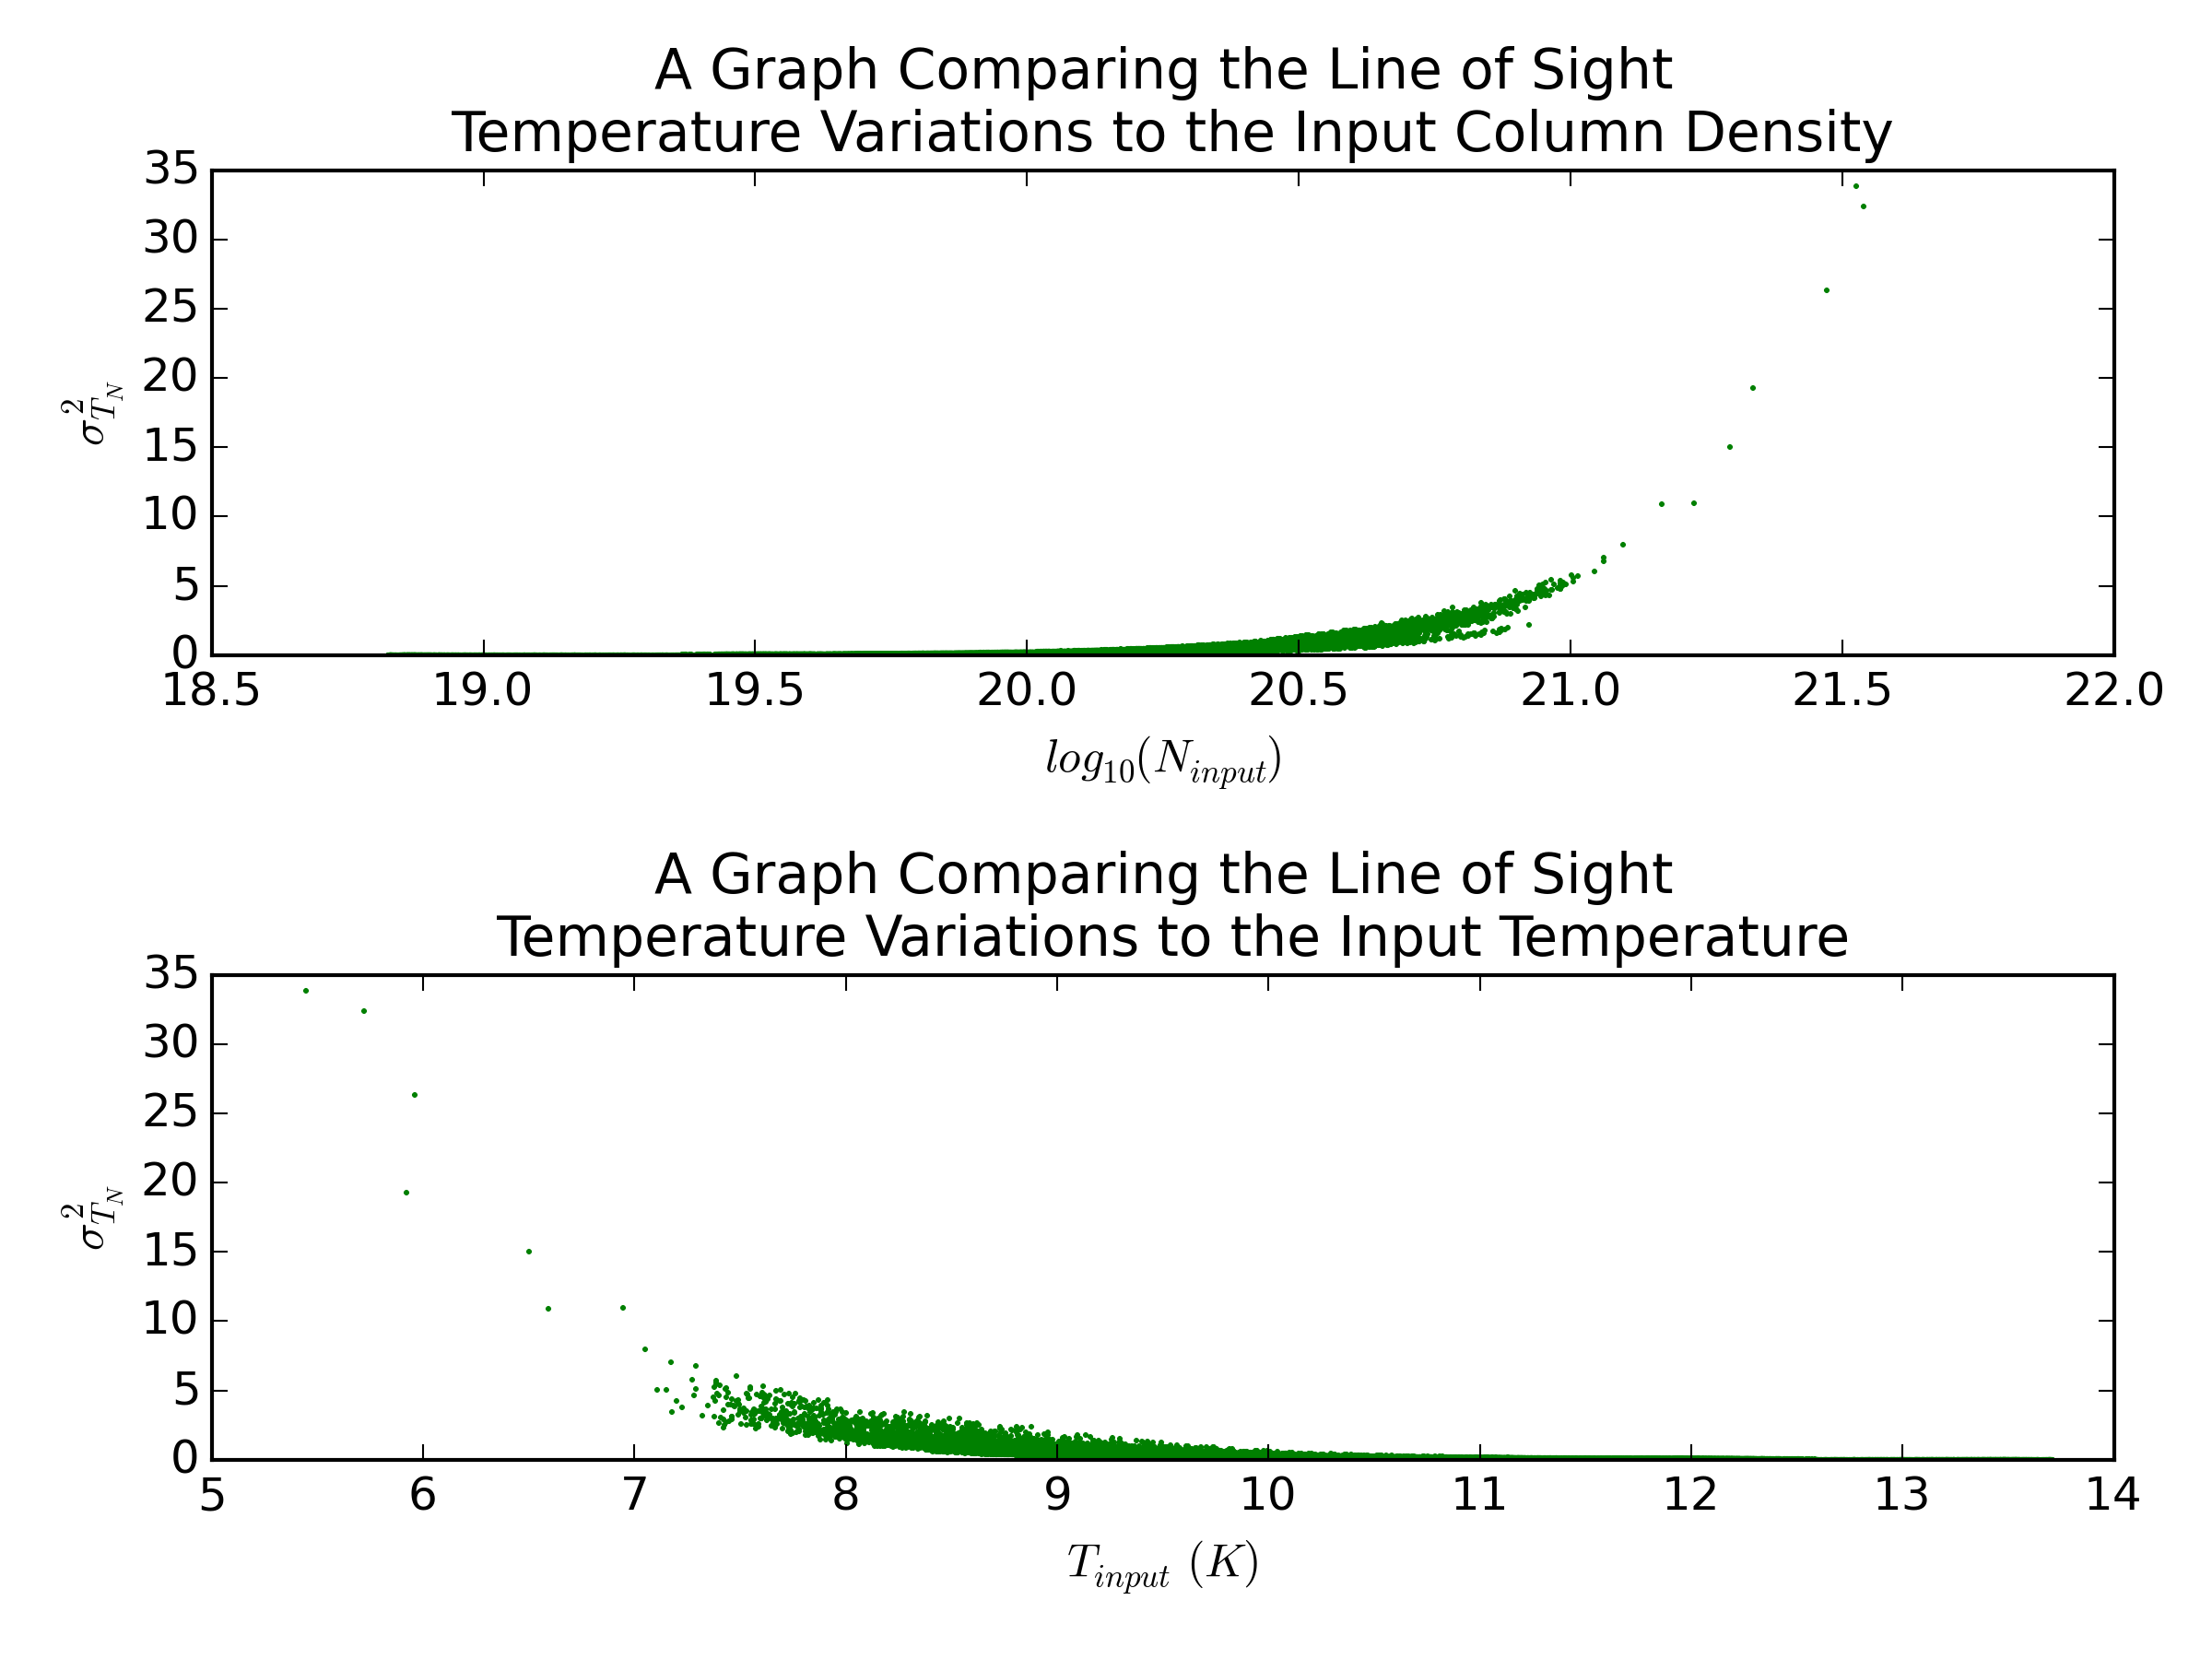
\includegraphics[width=\linewidth]{../img/sph/sigma_T_inp.png}
  \caption{The line of sight temperature variations in the Arepo simulation case as a function of the data derived $N$ and $T$.}\label{fig:sph_los}
\endminipage
%\caption{A figure comparing recovered and derived values of $N$ and $T$ and how they compare. Figure \ref{fig:iso_T} shows an overestimate of the $\chi^{2}$ recovered T whilst Figure \ref{fig:iso_N} shows an underestimate the $\chi^{2}$ recovered $N$.}
\end{figure}

Figure \ref{fig:iso_los} clearly shows minimal line of sight temperature variations in the isothermal sphere. The greatest temperature variation occurs close to high $N$, whilst there is very little (if any) temperature variation at low $N$. Likewise the data derived temperature shows the inverse: there is far greater line of sight temperature variation at low $T$ than there is at high $T$. Referring to Figure \ref{fig:map_N_data} we observe that the greatest column density is towards the centre of the sphere (likewise Figure \ref{fig:map_T_data} shows that the lowest temperature is in the same location) and the lowest column density is towards the image corners (greatest temperature is in these locations as well). These regions are of constant temperature (in this case, $15\/K$) so minimal temperature variation is expected. The high column density region has a larger line of sight temperature variation owing to, as Figure \ref{fig:col} demonstrates, the larger number of boundary regions that the line of sight intercepts. Whilst the isothermal sphere does not have distinct intersections of changing dust density, it is spherical and therefore further away from the image centre `sees` less of the sphere itself and more of the surrounding background. Of note here is the sharp drop off in $\sigma^{2}$ at very high $N$. To understand this, we must consider the image boundaries. By referring again to Figure \ref{fig:map_T_data}, we see that the regions that lie within this $N$ range essentially `touch` the image boundaries. In 3-dimensional parameter space, this means that this point does not have any of the simulated background infront of (or behind it). This produces constant temperature along the line of sight, resulting in the sharp drop off observed. The curvature of the sphere results in points around this central `touch` point having background material infront of and behind, therefore increasing the line of sight temperature variation. Figure \ref{fig:map_T_data} shows that a large portion (out to $~$ $100 pixels$ remains at a column density cloe to $10^{20}\/cm^{-2}$). This corresponds to the peak in the temperature variation - the drop off in $\sigma^{2}$ then occurs from here as more of the background is seen along the line of sight. The other minimum in $\sigma^{2}$ is found to be at low $N$, where the background exists.

Repeating the same procedure on the Arepo data produces Figure \ref{fig:sph_los}. The same behaviour as was observed in Figure \ref{fig:iso_los} is observed here: $\sigma^{2}$ increases with $N$ and decreases with $T$. The constraining of $\sigma^{2}$ in $N$ is remarkbly minimal, whilst the scatter of
$\sigma^{2}$ in $T$ is far greater. This is to be expected, as the input temperature varies along the line of sight for more in the Arepo instance than in the isothermal instance. We observe far greater temperature variations in Arepo data than in the isothermal sphere. This is to be expected, given the large range of temperatures (those derived from the input quanitites) in the Arepo data.

Interestingly in Figure \ref{fig:sph_los} we do not observse the sharp drop off in $\sigma^{2}$ at high $N$ that is seen in Figure \ref{fig:iso_los}. This is to be expected however as the structure in Arepo data is transient and therefore not of uniform, spherical shape.

\section{Core extraction}
Applying \texttt{astrodendro} to the column density maps in Figures \ref{fig:map_N_chi_sph} and \ref{fig:map_N_data_sph} produces Figures \ref{fig:chi_dendro} and \ref{fig:data_dendro}.

\begin{figure}[H]
\minipage{0.4\textwidth}
  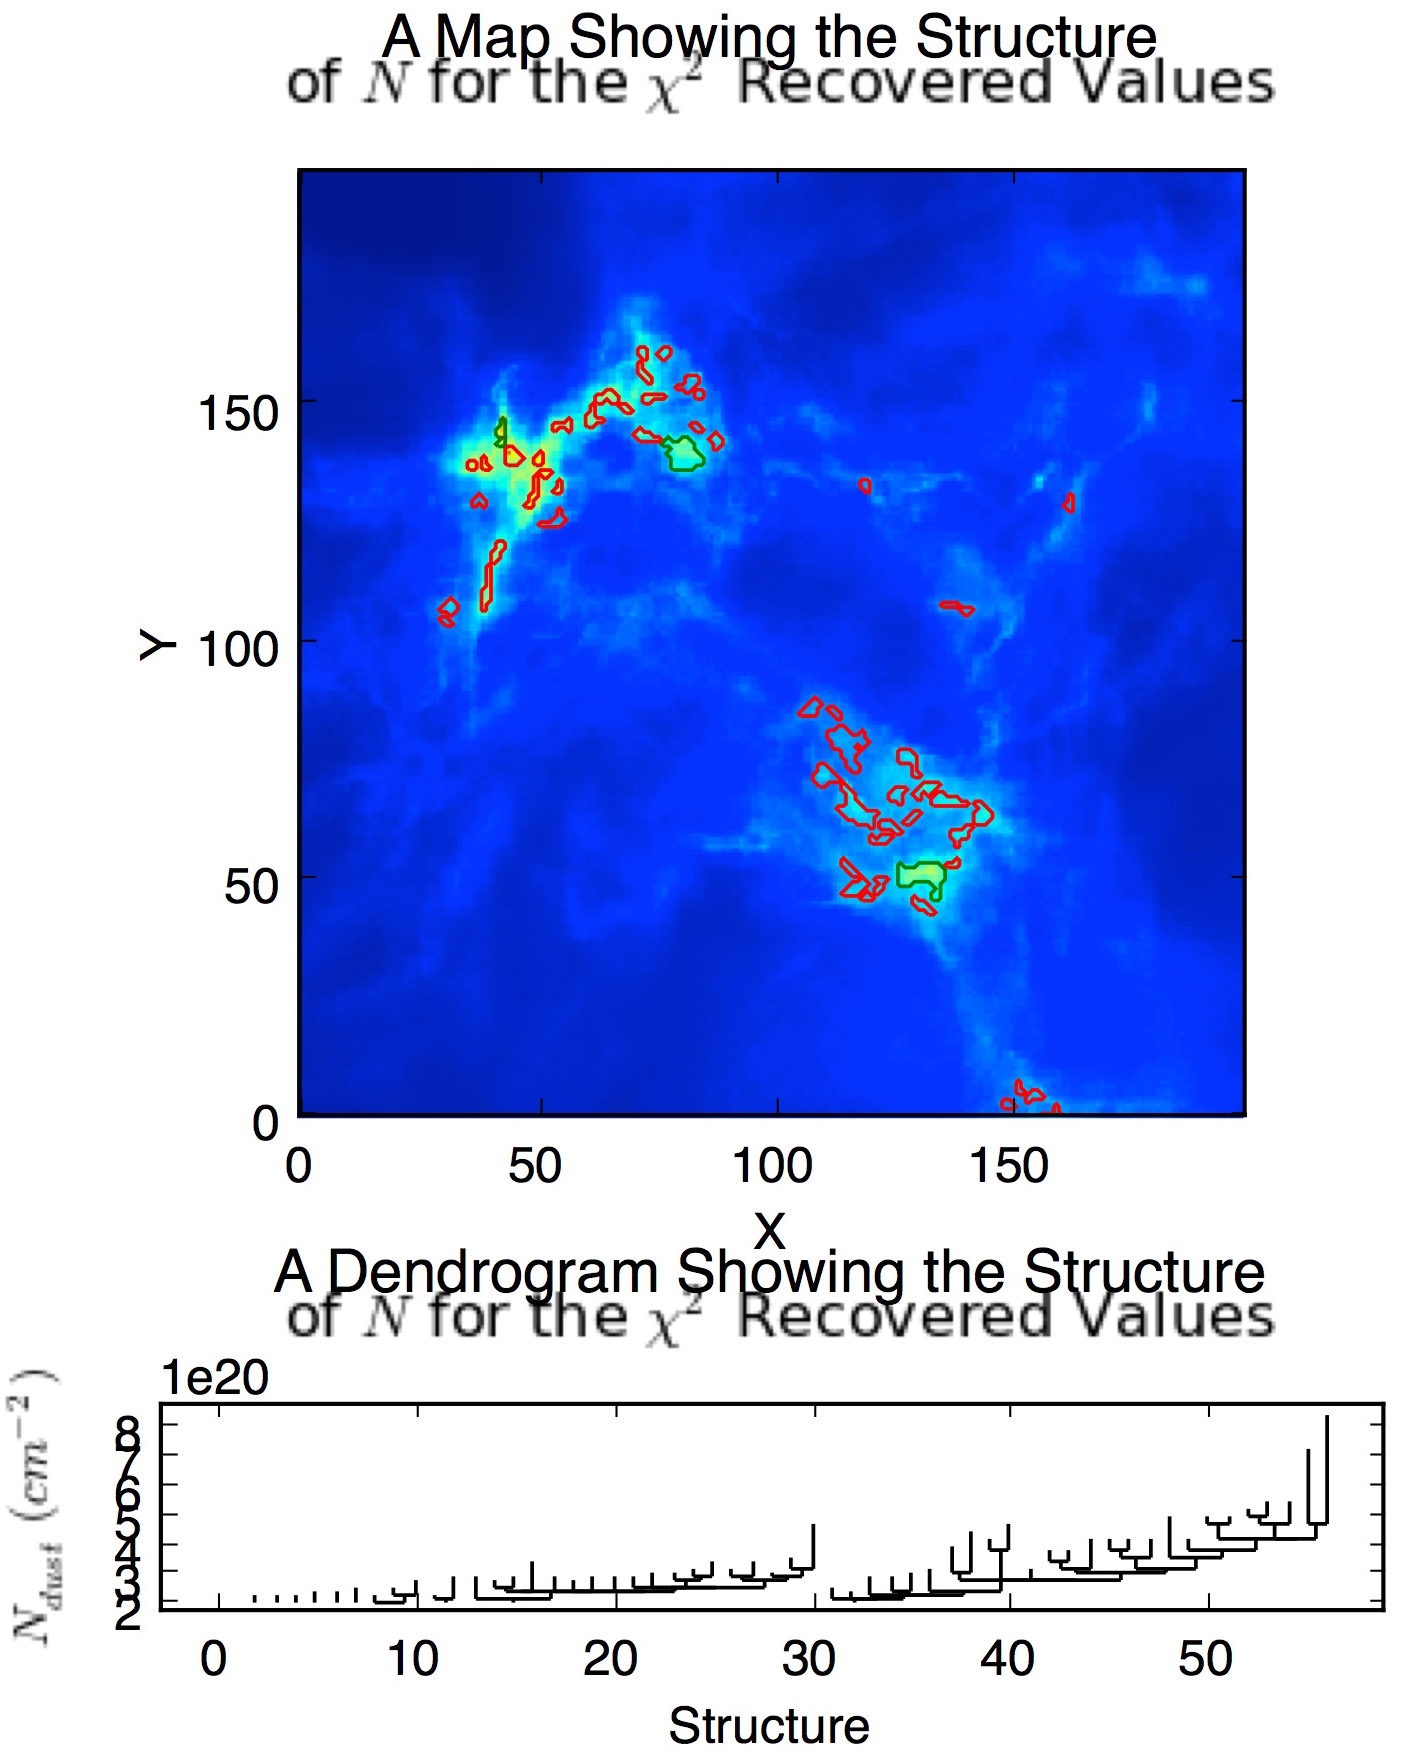
\includegraphics[width=\linewidth]{../img/N_chi_inp.jpg}
  \caption{The $\chi^{2}$ recovered $N$. The contours represent leaves of the dendrogram: a red contour represents an unbound core, whilst a green contour represents a bound core. The lower graph shows the dendrogram. In this case, it displays the structure of the leaves (cores).}\label{fig:chi_dendro}
\endminipage\hfill
\minipage{0.4\textwidth}
  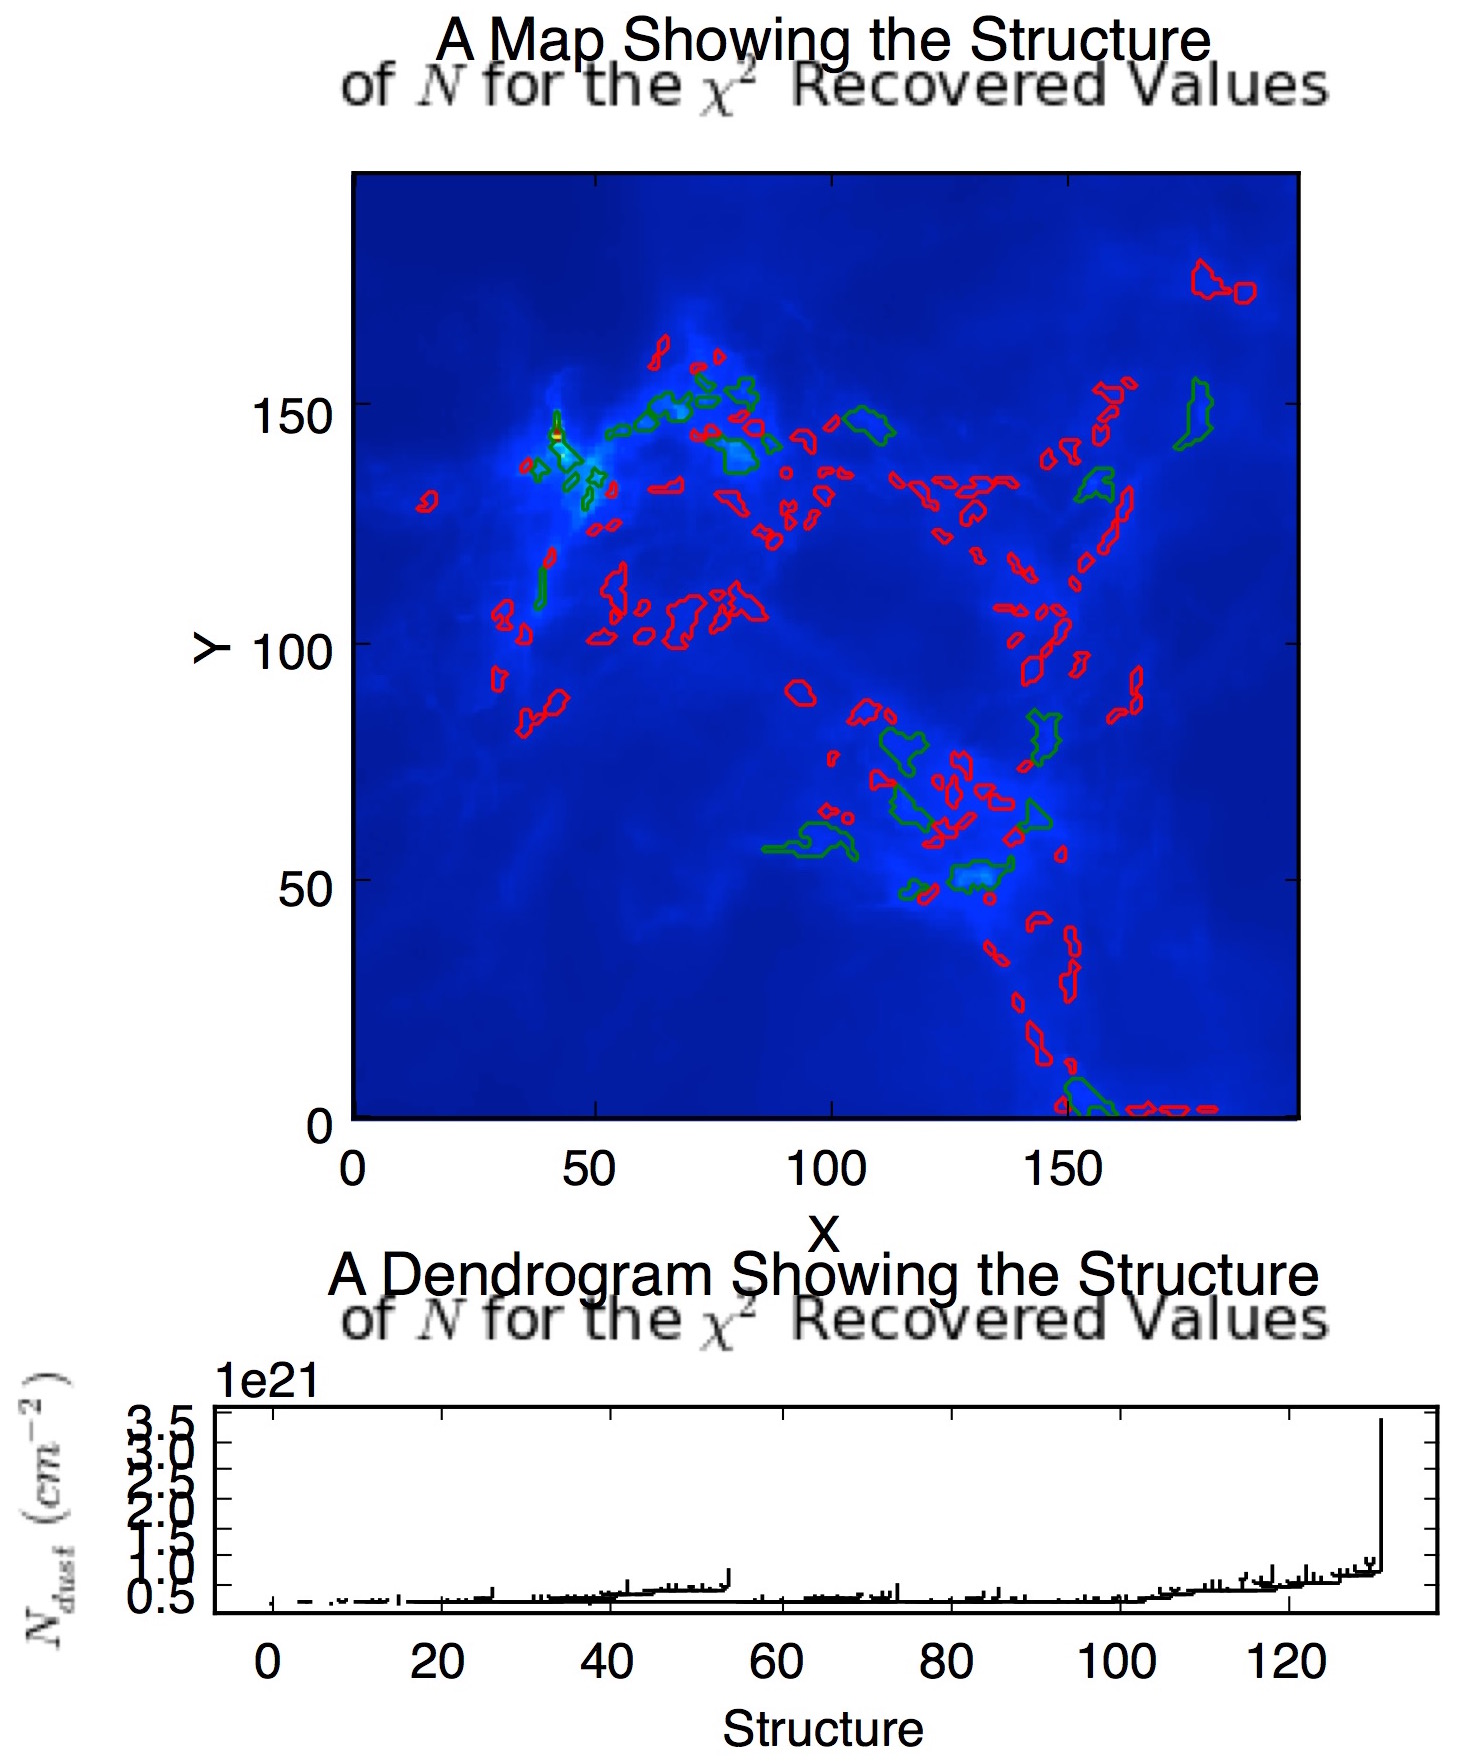
\includegraphics[width=\linewidth]{../img/N_data_inp.jpg}
  \caption{The data derived $N$. The contours represent leaves of the dendrogram: a red contour represents an unbound core, whilst a green contour represents a bound core. The lower graph shows the dendrogram. In this case, it displays the structure of the leaves (cores).}\label{fig:data_dendro}
\endminipage
%\caption{A figure comparing recovered and derived values of $N$ and $T$ and how they compare. Figure \ref{fig:iso_T} shows an overestimate of the $\chi^{2}$ recovered T whilst Figure \ref{fig:iso_N} shows an underestimate the $\chi^{2}$ recovered $N$.}
\end{figure}

The conditions to extract these cores are discussed in Section \ref{sec:conditions}. Figure \ref{fig:chi_dendro} displays 3 bound cores, whilst Figure \ref{fig:data_dendro} displays 25 bound cores. The 3 bound cores extracted from the $\chi^{2}$ $N$ (Figure \ref{fig:chi_dendro}) are also extracted from the data derived $N$
(Figure \ref{fig:data_dendro}). Table \ref{table:mass} shows the masses for the cores recovered in both dendrograms.

\begin{table}[h]
  \centering
   \begin{tabular}{||c c||}
   \hline
   $M_{\chi^{2}}/M_{Sun}$ & $M_{data}/M_{Sun}$ \\ [0.5ex]
   \hline\hline
   $0.3403+/-0.3616$    & $0.7016$     \\
   \hline
   $0.2799+/-0.3269$  & $0.6241$ \\
   \hline
   $0.1041+/-0.07105$  & $0.7974$ \\
   \end{tabular}
   \caption{A table showing the masses of cores extracting from the $\chi^{2}$ $N$ map and the data derived $N$ map.}
   \label{table:mass}
\end{table}

The larger number of core extractions from the data derived $N$ is expected, as these values are larger than the $\chi^{2}$ equivalents. This is also apparent in the mass estimates from Table \ref{table:mass}, as the $M_{\chi^{2}}$ are consistently underestimated with respect to $M_{data}$. Again, this is to expected as the column densities (and therefore mass) is lower in the $\chi^{2}$ case relative to the data derived case.

The dendrograms in Figures \ref{fig:chi_dendro} and \ref{fig:data_dendro} show similar shapes - evidence that the $\chi^{2}$ routine retains the substructure evident in the data. The dendrogram in Figure
\ref{fig:data_dendro} extends to a greater $N$ - this is due to the fact that the $\chi^{2}$ routine fails to pick up the small, dense regions of the map. However, \textcite{coldensity} finds that the minimum density required for star formation to occur is $10^{21}\/cm^{-2}$. All of the regions highlighted in Figures \ref{fig:chi_dendro} and \ref{fig:data_dendro} exceed this limit, implying that the cores observed are indeed sites of star formation.

%-----------------------------------------------------------------
% Discussion
%-----------------------------------------------------------------

\chapter{Discussion}
Section \ref{sec:iso} illustrates that whilst the $\chi^{2}$ recovered values of $N$ and $T$ remain close to their data derived counterparts (especially in the low $N$ and high $T$ regime), the minimisation routine still understimates $N$ and overestimates $T$. In comparison, Section \ref{sec:sph} shows largely the same: an accurate recovery of $N$ and $T$ in the low $N$ and high $T$ regime, though the same underestimate of $N$ and overestimate of $T$ is evident. Interestingly, Figure \ref{fig:contours} displays the same relationship as observed in \textcite{noise,noiseb} who attribute this behaviour to noise in the observations. \textcite{noise,noiseb} does however note that this behaviour could be a property of the emitting dust and not, as is first stated, a noise effect. The study shown here would imply that the latter is true, given that the observations used here are based upon the Arepo simulation which has no traditional noise (e.g. Poission noise, dark currents etc.) as would be the case in `real' observations. However, noise is still emergent in these results owing to the line of sight temperature variations, meaning the source of the elliptical $\chi^{2}$ values could stem from here.

Interestingly the largest departure from the data derived value is when the column density $N$ is high and the temperature $T$ is low. Referring to Figure \ref{fig:col}, high $N$ along the line of sight occurs when there are a number of different boundaries, where a boundary is an increase/decrease in density from one medium to another. Given that high density regions are heated less, and therefore have a lower temperature $T$, we observe that regions of high $N$ are also regions of large temperature variation. This is observed in Figure \ref{fig:iso_los} and \ref{fig:sph_los}, which shows the standard deviation in temperature along the line of sight. The largest variation is observed to be at high $N$ and at low $T$, with that variation exhibiting an expotential behaviour. Furthermore, the large temperature variations render the single $T$ modified blackbody being fit to the data an inaccurate assumption. Even in the isothermal case where we observe very minimal temperature variations, $T$ is still overestimated. \textcite{noise,noiseb} also find that this effect is worse when fitting to low $\lambda$ data, hence the inaccurate values of $N$ and $T$ derived when using both the SPIRE and PACS bands to fit using $\chi^{2}$.

Whilst the PDFs in Figures \ref{fig:map_N_chi} and \ref{fig:map_N_data} exhibit the same shape, their power-law tails are interesting. \textcite{tail} states that the PDF is best described by a lognormal in the turbulent region (central to the PDF), where gravity is yet to cause the gas to collapse. This relationship is observed here in Figures \ref{fig:map_N_chi} and \ref{fig:map_N_data}. This region is observed to have a power-law relationship \parencite{powerlaw}, which is thought to arise from the effect of gravity in the cold and molecular regions of the cloud. One could presume, therefore, that the presence of such a power-law here implies a contribution from gravitationally bound material. We observe from our dendrogramic extraction that gravitationally bound cores do indeed exist within the cloud, though the number of gravitationally bound cores extracted from both maps is inconsistent despite both extracting 3 of the same cores. The tail drop off in Figure \ref{fig:map_N_chi} falling below the drop off in Figure \ref{fig:map_N_data} lends credence to this, in so far as significantly fewer cores are extracted from Figure \ref{fig:map_N_chi} (i.e. the $\chi^{2}$ recovered values) than from Figure \ref{fig:map_N_data} (i.e. the data derived values). Were $\chi^{2}$ to recover more high $N$ material, it may extract more cores thereby extending the power-law tail. As \textcite{tail} highlights, the peak in the PDF is attributable to the warmer, atomic material whilst the tail is attributable to the cold, molecular material. We find that the lack of high $N$ and low $T$ material - the material responsible for the power-law tail - severely limits a $\chi^{2}$ test`s ability to extract cores that exist in this region of the PDF. Furthermore the underestimate of $N$  results in a lower mass determined from the $\chi^{2}$ (owing to Equation \ref{eq:mass_dendro}) relative to the data derived $N$.

Given the core masses the CMF could be plotted, however the lack of extracted cores in the project meant that this wasn't possible. Further surveys (on either real data or larger synthetic data) would be required to build a set of cores large enough to plot an accurate CMF.

%-----------------------------------------------------------------
% Conclusion
%-----------------------------------------------------------------

\chapter{Conclusion}
In summary we have demonstrated, by constructing maps of column density $N$ and temperature $T$ from simulated molecular clouds, that the $\chi^{2}$ recovered values are underestimated in $N$ and overestimated in $T$ with respect to the values of $N$ and $T$ determined from the initial input conditions used to produce the simulation. We have found that this is the case even in the absence of large line of sight temperature variations and observational noise. Furthermore we have generated dendrograms of the constructed maps in order to extract the prestellar cores that exist within them, finding that both $\chi^{2}$ $N$ and data derived $N$ contain differing numbers of gravitationally bound cores (3 in the $\chi^{2}$ case and 25 in the data derived case), despite extracting 3 of the same cores across both values. This was attributed to the $\chi^{2}$ minimisation failing to detect high $N$ material, thereby halting the power-law tail observed in the $log_{10}(N)$ PDFs therefore destroying evidence of cores at these densities. The core masses that were recovered from $\chi^{2}$ were found to be underestimated relative to the data derived masses.

%-----------------------------------------------------------------
% Future Work
%-----------------------------------------------------------------

\chapter{Future work}
Future work would focus on applying this technique to constraining the CMF, either through further simulated data or through real observations. Work would also commence on assessing how statistically valid the $\chi^{2}$ recovered values of $N$ $T$ are in relation to their data derived (and therefore `true`) counterparts.

Future work would also focus on adding further variables to the simulation. This study considered 1 dust species: silicate grains. Adding further dust species, as well as gas, to the simulation would allow an analysis of dust and gas column density across both the image space itself as well as the sites isolated as cores by the dendrogram. When paired with a thermal Monte-Carlo simulation, the inclusion of gas would allow the effect of gas-dust temperature coupling on recovered $N$ and $T$ to be assessed. These proposals would also allow further study into the elliptically shaped $T-N$ graph as found by \textcite{noise,noiseb}.

%-----------------------------------------------------------------
% Acknowledgements
%-----------------------------------------------------------------

\chapter{Acknowledgements}
I would like to thank Dr. Paul Clark for his guidance and encouragement as well as his proof-reading and advice (relating to both this project and matters external) throughout this academic year. I would also like to thank Dr. Sarah Ragan for her Python assistance and observational advice throughout the project. This project made heavy use of the Python programming language, RADMC-3D and astrodendro and their accompanying handbooks, web resources and tutorials.

%-----------------------------------------------------------------
% Appendix
%-----------------------------------------------------------------

\chapter{Appendix}

\section*{Code}
All code was version controlled using GitHub and stored in a private repository throughout development. The repository containing all code can be found at \href{http://www.github.com/tomasjames/ZiggyStarDust}{http://www.github.com/tomasjames/ZiggyStarDust}. Below is the $\chi^{2}$ fitting routine used in this project:\texttt{chiv6.py}. All further code used can be found at the GitHub repository above.

\subsection*{\texttt{chiv6.py}}
\lstinputlisting[basicstyle=\ttfamily\scriptsize,language=Python]{../code/chiv6.py}

\section*{Dust heating}
\textcite{treecol} defines $\Gamma_{ext}$ due to the ISRF alone to be:

\begin{equation}
  \Gamma_{ext} = \chi \Gamma_{ext,0}
\end{equation}

$\Gamma_{ext,0}$ defines an optically thin (i.e. $\tau<<1$) heating rate whilst $\chi$ is a dimensionless scaling factor that accounts for the attenuation of the ISRF by dust emission. $\Gamma_{ext,0}$ is defined as:

\begin{equation}
  \Gamma_{ext,0} = 4\pi R_{dust-gas} \rho \int_{0}^{\inf} J_{\nu} \kappa_{\nu} d\nu
\end{equation}

$_{dust-gas}$ is the dust to gas ratio, whilst $\rho$ is the gas density. $J_{\nu}$ is the mean specific intensity of the ISRF, and $\kappa_{\nu}$ is the dust opacity. The cooling rate is defined similarly:

\begin{equation}
  \Lambda_{dust} = 4\pi R_{dust-gas} \rho \int_{0}^{\inf} B_{\nu} \kappa_{\nu} d\nu
\end{equation}

The only emergent difference between the equations is the integrand: $B_{\nu}$ is the Planck function for a particle at temperature $T_{d}$.

%-----------------------------------------------------------------
% Bibliography
%-----------------------------------------------------------------

\printbibliography

%\nocite{*}
%\printbibliography

%-----------------------------------------------------------------
% Appendix
%-----------------------------------------------------------------

\end{document}
